\documentclass[a4paper,12pt]{article}
\usepackage[utf8]{inputenc}
\usepackage[english,russian]{babel}
\usepackage[T2A]{fontenc}
\usepackage[left=1cm,right=1cm,
top=1cm,bottom=1cm,bindingoffset=0cm]{geometry}
\usepackage{amsmath}
\usepackage{amsfonts}
\usepackage{amssymb}
\usepackage{amsthm}
\usepackage{graphicx}
%pdf search
\usepackage{cmap}
\usepackage{verbatim}
\usepackage{epigraph}
\usepackage{wasysym}
%\usepackage{hyperref}
\usepackage{mathrsfs}
\title{Путевые заметки о билетах к экзамену по анализу}
\date{13.01.2015}
\author{}

\newcommand\R{\mathbb{R}} 
\newcommand\Q{\mathbb{Q}}
\newcommand\Z{\mathbb{Z}}
\newcommand\N{\mathbb{N}}

\newcommand\ilim{\lim\limits}
\newcommand\convex{\,\underline\cup\,}
\newcommand\concave{\,\overline\cap\,}

\theoremstyle{plain}
\newtheorem{thrm}{Теорема}
\newtheorem{lem}{Лемма}
\newtheorem{stat}{Утверждение}
\newtheorem{imp}{Следствие}

\theoremstyle{definition}
\newtheorem{defn}{Определение}
\newtheorem{exmp}{Пример}

\theoremstyle{remark}
\newtheorem{rem}{Замечание}

\newenvironment{ittproof}{$\square$ }{ $\blacksquare$ \\}
\newenvironment{itlproof}{$\phantom{0}\\ \blacktriangledown$ \\ }%
{ \phantom{0}\\ $\blacktriangle$ \\}


\def\resetdefs{ \setcounter{defn}{0}\setcounter{exmp}{0} }
\def\resetthrm{ \setcounter{thrm}{0}\setcounter{stat}{0} }
\def\resetrem{ \setcounter{rem}{0} }
\def\resetall{ \resetdefs \resetthrm \resetrem}

\def\itemrange#1{%
  \addtocounter{enumi}{1}%
  \edef\labelenumi{\theenumi--\noexpand\theenumi.}%
  \addtocounter{enumi}{-1}%
  \addtocounter{enumi}{#1}%
  \item
  \def\labelenumi{\theenumi.}
}
\begin{document}

\maketitle
\epigraph{\sl Матан осилит ботающий }{}
\section*{Пределы}
\begin{enumerate}
  \setcounter{enumi}{18}
  \item Сходимость в себе
    { \defn $(x_n)$ называется сходящейся в себе (фундаментальной), если
      \[
        \forall\,\varepsilon>0 \exists\,N:\forall\,m,n > N\; |x_n - x_m| < \varepsilon 
      \] 
    }
    { \lem\label{lem:fund_implies} $(x_n)$ сходится $\Rightarrow$ $(x_n)$"---~фундаментальная. }
    { \lem\label{lem:fund_limited} Если последовательность сходится в себе, то ограничена она }
    \begin{itlproof}
      Рассмотрим $\varepsilon=1$, тогда $\forall\, n,m > N\; |x_n - x_m| < 1$.
      Зафиксируем $m$, ведь для любых же верно.
      Тогда $x_m-1 < x_n < x_m + 1$. Тогда число элементов снаружи ограничено.
      Выберем из них максимальный и минимальный"---~победа.
    \end{itlproof}
    \begin{thrm}[Больцано--Коши]
      $(x_n)$"---~фундаментальная $\Leftrightarrow$ $x_n\xrightarrow[n\to\infty]{} L$
    \end{thrm}
    \begin{ittproof}
      \begin{description}
        \item[\fbox{$\Leftarrow$} :]  см. лемму~\ref{lem:fund_implies}
        \item[\fbox{$\Rightarrow$} :] по лемме~\ref{lem:fund_limited} $\exists\,A,B:A\leq x_n\leq B$.
          Тогда из неё можно выбрать сходящуюся подпоследовательность $x_{n_k}\to L$.
          \begin{align*}
            &\forall\,\varepsilon>0 \exists\,N : \forall\, m,n > N \; |x_m-x_n| < \varepsilon \\
            &\forall\,\varepsilon>0 \exists\,K : \forall\, k > K \; |x_{n_k} - L| < \varepsilon 
          \end{align*}
          Пусть $M = \max{K,N}$, $m = n_k$. 
          Тогда $k > M \Rightarrow n_k \geq k > M \geq N$, $|x_n - x_m| < \varepsilon$.
          \[
            k > M \Rightarrow k \geq K \Rightarrow |x_{n_k} - L | = |x_m - L| < \varepsilon \\
            |x_n - L| = |x_n - x_m + x_m - L| \leq |x_n - x_m | + |x_m - L| < 2\varepsilon 
          \]
      \end{description}
    \end{ittproof}
\end{enumerate}

\section*{Непрерывности}

\begin{enumerate}
  \setcounter{enumi}{19}
  \item Непрерывность, разрывы
    { \defn $f : A \to \R$ непрерывная в $x_0 \in A$}
    { \defn Непрерывность на промежутке }
    { \defn Изолированная точка, точка сгущения }
    { \defn Разрыв
      \begin{enumerate}
        \item 1 рода: 
          \begin{equation*}
            \left\{
            \begin{array}{l}
              f(x_0-0) , f(x_0 + 0) \; \text{оба существуют}\\ 
              f(x_0-0) = f(x_0 + 0) \neq f(x_0) 
            \end{array}
            \right.
          \end{equation*}
        \item 2 рода:\\
          Хотя бы один предел не существует или бесконечен
      \end{enumerate}
    }
    Свойства непрерывности:
    \begin{enumerate}
      \item $f, g \in C(x_o) \Rightarrow f \pm g , f\,g, 
        {f \over g}, |f| \in C(x_0)$
      \item $f \in C(x_0), g \in C(f(x_0), f : X \to Y, g : Y \to \R 
        \Rightarrow g \circ f \in C(x_0)$ 
    \end{enumerate}
  \item Теорема Больцано-Коши
    { \thrm Пусть $f : [a;b] \to [A;B],\; f \in C([a,b])$ . 
      Тогда $ \forall C \in [A;B]\; \exists c \in [a;b] : f(c) = C $
    }
  \itemrange{1} Теоремы о монотонной функции на промежутке и её разрывах
    \resetall
    { \thrm Пусть $f:I\to\R,\;I$~---промежуток и $f$ монотонна на $I$.
    Тогда все её разрывы~--- скачки }
    { \thrm Пусть $I \in\R $~---промежуток, $f\in C(I)$. Тогда и $f(I)$~--- промежуток }
    { \thrm Пусть $f:I \to\R,\;I$~---промежуток, $f$ монотонна. 
      Тогда и $f(I)$~--- промежуток $\Leftrightarrow f\in C(I)$ }
    { \thrm Пусть $f:I\to\R, f\in C(I)$~----строго монотонная функция.
      Тогда $\exists\,f^{-1}$, тоже строго монотонная, непрерывная на $I$, 
      с такой же монотонностью, что и $f$ }
  \item Корень
  \item Экспонента
    \resetall
    { \defn Пусть $x=n\in\N$. Тогда $a^n := \underbrace{a\cdot\dots a}_{n\text{ раз}}$. }
    { \defn Пусть $x=m\in\Z\setminus\N$. Тогда:
      \begin{description}
        \item[$x=0$:] $a^x := 1 $
        \item[$x<0$:] $a^x := {1\over a^{-x}}$
      \end{description} }
      { \defn Пусть $x={m\over n}\in\Q$. Тогда $a^x := \root n \of {a^m}$. }
      { \defn Пусть $x=\in\R$. Тогда 
        \begin{description}
          \item[$a > 1$:] $a^x := \sup\limits_{r\in\Q}\{a^r\,|\, r\leq x\}$
          \item[$a = 0$:] $a^x := 1$
          \item[$0 < a < 1$:] $a^x := \left({1\over a}\right)^{-x}$
        \end{description}
      }
      
      { \lem\label{lem:varbernineq} Пусть $a>1,\; n\in\N$. Тогда $a^{1/n}-1 \leq {a-1\over n}$ }

      \begin{thrm}\label{thrm:exponent}
        Пусть $f(x) = a^x =: \exp_a(x),\;x\in\R,\;a>0$.
        Тогда:
        \begin{enumerate}
          \item $f:\R\to(0;+\infty)$
          \item $f \uparrow \text{ при }a > 1$ и $f\downarrow \text{ при } 0 < a < 1$
          \item $f(x+y) = f(x)\cdot f(y)$
          \item $f\in C$
        \end{enumerate}
      \end{thrm}
      \begin{ittproof}
        \begin{enumerate}
          \item\label{item:exp_values} $f:\R\to(0;+\infty)$ \\
            Пусть $y_0\in\R_+$
            \[
              \sphericalangle\; A=\{x\in\R\,|\,a^x < y_0\} \text{ и } 
              B = \{x\in\R\,|\,y_0 < a^x\}
            \]
            Эти множества не пусты, в них есть хотя бы рациональные числа.
            Из пункта~\ref{item:exp_monot} одно правее другого. 
            Тогда из аксиомы полноты 
            $\forall x_1\in A,\: x_2\in B \; \exists\, x_0: x_1\leq x_0\leq x_2$.
            Осталось доказать только, что $a^{x_0} = y_0$, а это почти как теорема о $\sqrt{2}$.
            Разве что добавку можно взять равной $1/n$.
          \item\label{item:exp_monot} 
            $a > 1,\; x_1,x_2\in\R \; x_1 < x_2\Rightarrow a^{x_1} < a^{x_2} $ \\
            По теореме о плотности $\Q : \; \exists\,r_1,r_2\in\Q : x_1<r_1<r_2<x_2$,
            $\exists\, r_3\in\Q : r_2 < r_3 < x_2$.
            Тогда 
            \begin{align*}
              &a^{x_1} = \sup\{a^r\,|\,r\leq x_1\} < a^{r_1} \\
              &r_2 < r_3 < x_2 \Rightarrow a^{r_2} < a^{r_3} \Rightarrow 
              a^{x_2} = \sup\{a^r\,|\,r\leq x_2\} > a^{r_2} 
            \end{align*}
            Таким образом $a^{x_1} < a^{r_1} < a^{r_2} < a^{x_2}$.
          \item\label{item:exp_oper} $f(x+y) = f(x)\cdot f(y)$
            Следует из аналогичного свойства для рациональных чисел по~\ref{item:exp_cont}
          \item\label{item:exp_cont} $f\in C$
            Из принципа Архимеда $\exists\, n : |x-x_0| < {1\over n}$.
            Также $\exists\,r_1,r_2\in\Q:r_1 < x < x_0 < r_2$, $|r_1 - r_2| < 1/n$.
            Тогда по~\ref{item:exp_monot} \[
              a^{r_1} < a^{x_1} < a^{x_0} < a^{r_2} \Rightarrow 
              0 < a^{x_0} - a^{x} < a^{r_2} - a^{r_1} < a^{r_1}(a^{r_2-r_1}-1) <
              a^{r_1}\left( {a-1\over n} \right) < \varepsilon
            \]
        \end{enumerate}
      \end{ittproof}
  \item Логарифм и степенная функция
  \item О-символика 
    \resetall
    { \defn $ f(x) = o(g(x)) \text{ при } x \to c 
      \Leftrightarrow \lim\limits_{x \to c}{f(x) \over g(x)} = 0$ }
    
    { \defn $ f(x) = O(g(x)) \text{ при } x \to c 
      \Leftrightarrow \; \exists M : \lim\limits_{x \to c}{|f(x) \over g(x)|} \leq M $ }
    
    { \defn $ f(x) \sim g(x) \text{ при } x \to c 
      \Leftrightarrow \lim\limits_{x \to c}{f(x) \over g(x)} = 1$ } \\
    \begin{table}[h]
      \centering
      \begin{tabular}{lll}
        $\ilim_{x \to 0}{\sin x \over x} = 1$ & $x \sim \sin x$ & $\sin x - x = o(x)$\\
        $\ilim_{x \to 0}{1 - \cos x \over x^2} = {1\over2}$ & ${x^2 \over 2} \sim \cos x$ 
        & $\cos x - 1 - {x^2 \over 2} = o(x^2)$\\
        $\ilim_{x \to 0}{\ln(x+1) \over x} = 1$ & $x \sim \ln(x+1)$ & $\ln(x+1) - x = o(x)$\\
        $\ilim_{x \to 0}{e^x - 1\over x} = 1$ & $e^x \sim 1 + x$ & $e^x  = 1 + x + o(x)$
      \end{tabular}
      \caption{Полезные пределы}
      \label{tab:lims}
    \end{table}
  \item Теорема Вейерштрасса
    \begin{thrm}\label{thrm:Weierstrass_cont}
      Пусть $f\in C([a;b])$. Тогда $f$ ограничена и достигает своих 
      \raisebox{0.5ex}{наибольшего} и \raisebox{-0.5ex}{наименьшего} 
      значений. 
    \end{thrm}
    \begin{ittproof}
      Нетрудно понять, что $\exists\,y_n\in f([a;b]):y_n\to\sup\limits[a;b]f(x) = s$.
      Из теоремы Больцано--Коши $\exists\,x_n\in[a;b]:y_n=f(x_n)$. А из $x_n$ можно вытащить
      $x_{n_i} \to c \Rightarrow y_{n_i}=f(x_{n_i}) \to f(c)$ по непрерывности $f$.
      А по теореме о пределе подпоследовательности $f(c)=s$. Ограниченность очевидна.
      Для инфимума тоже самое.
    \end{ittproof}
  \item Равномерная непрерывность и теорема Кантора
    \resetall
    { \defn $f : X \to \R \text{ равномерно непрерывна } \Leftrightarrow \\
    \Leftrightarrow 
    \forall \varepsilon > 0 \exists \delta > 0 \forall x_1 \in X \forall x_2 \in X
    |x_1 - x_2 | < \delta \Rightarrow | f(x_1) - f(x_2) | < \varepsilon $ 
    }
    { \exmp $f(x) = \sin{1 \over x}$ помимо всех прочих её неприятных особенностей
    непрерывна на $(0;1)$, но не равномерно непрерывна там же ($E.\ g.\ \varepsilon=1 $) 
    \begin{figure}[h!]
      \centering
      % GNUPLOT: LaTeX picture
\setlength{\unitlength}{0.240900pt}
\ifx\plotpoint\undefined\newsavebox{\plotpoint}\fi
\begin{picture}(1500,900)(0,0)
\sbox{\plotpoint}{\rule[-0.200pt]{0.400pt}{0.400pt}}%
\put(130.0,82.0){\rule[-0.200pt]{4.818pt}{0.400pt}}
\put(110,82){\makebox(0,0)[r]{-1}}
\put(1419.0,82.0){\rule[-0.200pt]{4.818pt}{0.400pt}}
\put(130.0,276.0){\rule[-0.200pt]{4.818pt}{0.400pt}}
\put(110,276){\makebox(0,0)[r]{-0.5}}
\put(1419.0,276.0){\rule[-0.200pt]{4.818pt}{0.400pt}}
\put(130.0,471.0){\rule[-0.200pt]{4.818pt}{0.400pt}}
\put(110,471){\makebox(0,0)[r]{ 0}}
\put(1419.0,471.0){\rule[-0.200pt]{4.818pt}{0.400pt}}
\put(130.0,665.0){\rule[-0.200pt]{4.818pt}{0.400pt}}
\put(110,665){\makebox(0,0)[r]{ 0.5}}
\put(1419.0,665.0){\rule[-0.200pt]{4.818pt}{0.400pt}}
\put(130.0,859.0){\rule[-0.200pt]{4.818pt}{0.400pt}}
\put(110,859){\makebox(0,0)[r]{ 1}}
\put(1419.0,859.0){\rule[-0.200pt]{4.818pt}{0.400pt}}
\put(130.0,82.0){\rule[-0.200pt]{0.400pt}{4.818pt}}
\put(130,41){\makebox(0,0){-1}}
\put(130.0,839.0){\rule[-0.200pt]{0.400pt}{4.818pt}}
\put(457.0,82.0){\rule[-0.200pt]{0.400pt}{4.818pt}}
\put(457,41){\makebox(0,0){-0.5}}
\put(457.0,839.0){\rule[-0.200pt]{0.400pt}{4.818pt}}
\put(785.0,82.0){\rule[-0.200pt]{0.400pt}{4.818pt}}
\put(785,41){\makebox(0,0){ 0}}
\put(785.0,839.0){\rule[-0.200pt]{0.400pt}{4.818pt}}
\put(1112.0,82.0){\rule[-0.200pt]{0.400pt}{4.818pt}}
\put(1112,41){\makebox(0,0){ 0.5}}
\put(1112.0,839.0){\rule[-0.200pt]{0.400pt}{4.818pt}}
\put(1439.0,82.0){\rule[-0.200pt]{0.400pt}{4.818pt}}
\put(1439,41){\makebox(0,0){ 1}}
\put(1439.0,839.0){\rule[-0.200pt]{0.400pt}{4.818pt}}
\put(130.0,82.0){\rule[-0.200pt]{0.400pt}{187.179pt}}
\put(130.0,82.0){\rule[-0.200pt]{315.338pt}{0.400pt}}
\put(1439.0,82.0){\rule[-0.200pt]{0.400pt}{187.179pt}}
\put(130.0,859.0){\rule[-0.200pt]{315.338pt}{0.400pt}}
\put(1279,819){\makebox(0,0)[r]{$\sin\frac{1}{x}$}}
\put(1299.0,819.0){\rule[-0.200pt]{24.090pt}{0.400pt}}
\put(130,144){\usebox{\plotpoint}}
\put(130,144){\usebox{\plotpoint}}
\put(130,144){\usebox{\plotpoint}}
\put(130,144){\usebox{\plotpoint}}
\put(130,144){\usebox{\plotpoint}}
\put(130,144){\usebox{\plotpoint}}
\put(130,144){\usebox{\plotpoint}}
\put(130,144){\usebox{\plotpoint}}
\put(130,144){\usebox{\plotpoint}}
\put(130,144){\usebox{\plotpoint}}
\put(130,144){\usebox{\plotpoint}}
\put(130,144){\usebox{\plotpoint}}
\put(130,144){\usebox{\plotpoint}}
\put(130,144){\usebox{\plotpoint}}
\put(130,144){\usebox{\plotpoint}}
\put(130,144){\usebox{\plotpoint}}
\put(130,144){\usebox{\plotpoint}}
\put(130,144){\usebox{\plotpoint}}
\put(130,144){\usebox{\plotpoint}}
\put(130,144){\usebox{\plotpoint}}
\put(130,144){\usebox{\plotpoint}}
\put(130,144){\usebox{\plotpoint}}
\put(130.0,143.0){\usebox{\plotpoint}}
\put(130.0,143.0){\rule[-0.200pt]{0.723pt}{0.400pt}}
\put(133.0,142.0){\usebox{\plotpoint}}
\put(136,140.67){\rule{0.241pt}{0.400pt}}
\multiput(136.00,141.17)(0.500,-1.000){2}{\rule{0.120pt}{0.400pt}}
\put(133.0,142.0){\rule[-0.200pt]{0.723pt}{0.400pt}}
\put(137,141){\usebox{\plotpoint}}
\put(137,141){\usebox{\plotpoint}}
\put(137,141){\usebox{\plotpoint}}
\put(137,141){\usebox{\plotpoint}}
\put(137,141){\usebox{\plotpoint}}
\put(137,141){\usebox{\plotpoint}}
\put(137,141){\usebox{\plotpoint}}
\put(137,141){\usebox{\plotpoint}}
\put(137,141){\usebox{\plotpoint}}
\put(137,141){\usebox{\plotpoint}}
\put(137,141){\usebox{\plotpoint}}
\put(137,141){\usebox{\plotpoint}}
\put(137,141){\usebox{\plotpoint}}
\put(137,141){\usebox{\plotpoint}}
\put(137,141){\usebox{\plotpoint}}
\put(137,141){\usebox{\plotpoint}}
\put(137,141){\usebox{\plotpoint}}
\put(137,141){\usebox{\plotpoint}}
\put(137,141){\usebox{\plotpoint}}
\put(137,141){\usebox{\plotpoint}}
\put(137,141){\usebox{\plotpoint}}
\put(137,141){\usebox{\plotpoint}}
\put(137,141){\usebox{\plotpoint}}
\put(137,141){\usebox{\plotpoint}}
\put(137,141){\usebox{\plotpoint}}
\put(137,141){\usebox{\plotpoint}}
\put(137,141){\usebox{\plotpoint}}
\put(137,141){\usebox{\plotpoint}}
\put(137,141){\usebox{\plotpoint}}
\put(137,141){\usebox{\plotpoint}}
\put(137,141){\usebox{\plotpoint}}
\put(137,141){\usebox{\plotpoint}}
\put(137,141){\usebox{\plotpoint}}
\put(137,141){\usebox{\plotpoint}}
\put(137,141){\usebox{\plotpoint}}
\put(137,141){\usebox{\plotpoint}}
\put(137,141){\usebox{\plotpoint}}
\put(137,141){\usebox{\plotpoint}}
\put(137,141){\usebox{\plotpoint}}
\put(137,141){\usebox{\plotpoint}}
\put(137,141){\usebox{\plotpoint}}
\put(137,141){\usebox{\plotpoint}}
\put(137,141){\usebox{\plotpoint}}
\put(137,141){\usebox{\plotpoint}}
\put(137,141){\usebox{\plotpoint}}
\put(137,141){\usebox{\plotpoint}}
\put(137,141){\usebox{\plotpoint}}
\put(137,141){\usebox{\plotpoint}}
\put(137,141){\usebox{\plotpoint}}
\put(137,141){\usebox{\plotpoint}}
\put(137,141){\usebox{\plotpoint}}
\put(137,141){\usebox{\plotpoint}}
\put(137,141){\usebox{\plotpoint}}
\put(137,141){\usebox{\plotpoint}}
\put(137,141){\usebox{\plotpoint}}
\put(137,141){\usebox{\plotpoint}}
\put(137,141){\usebox{\plotpoint}}
\put(137,141){\usebox{\plotpoint}}
\put(137,141){\usebox{\plotpoint}}
\put(137,141){\usebox{\plotpoint}}
\put(137,141){\usebox{\plotpoint}}
\put(137,141){\usebox{\plotpoint}}
\put(137,141){\usebox{\plotpoint}}
\put(137,141){\usebox{\plotpoint}}
\put(137,141){\usebox{\plotpoint}}
\put(137,141){\usebox{\plotpoint}}
\put(137,141){\usebox{\plotpoint}}
\put(137,141){\usebox{\plotpoint}}
\put(137,141){\usebox{\plotpoint}}
\put(137,141){\usebox{\plotpoint}}
\put(137,141){\usebox{\plotpoint}}
\put(137,141){\usebox{\plotpoint}}
\put(137,141){\usebox{\plotpoint}}
\put(137,141){\usebox{\plotpoint}}
\put(137,141){\usebox{\plotpoint}}
\put(137.0,141.0){\rule[-0.200pt]{0.723pt}{0.400pt}}
\put(140.0,140.0){\usebox{\plotpoint}}
\put(140.0,140.0){\rule[-0.200pt]{0.723pt}{0.400pt}}
\put(143.0,139.0){\usebox{\plotpoint}}
\put(143.0,139.0){\rule[-0.200pt]{0.723pt}{0.400pt}}
\put(146.0,138.0){\usebox{\plotpoint}}
\put(146.0,138.0){\rule[-0.200pt]{0.723pt}{0.400pt}}
\put(149.0,137.0){\usebox{\plotpoint}}
\put(149.0,137.0){\rule[-0.200pt]{0.723pt}{0.400pt}}
\put(152.0,136.0){\usebox{\plotpoint}}
\put(152.0,136.0){\rule[-0.200pt]{0.723pt}{0.400pt}}
\put(155.0,135.0){\usebox{\plotpoint}}
\put(155.0,135.0){\rule[-0.200pt]{0.723pt}{0.400pt}}
\put(158.0,134.0){\usebox{\plotpoint}}
\put(158.0,134.0){\rule[-0.200pt]{0.723pt}{0.400pt}}
\put(161.0,133.0){\usebox{\plotpoint}}
\put(161.0,133.0){\rule[-0.200pt]{0.723pt}{0.400pt}}
\put(164.0,132.0){\usebox{\plotpoint}}
\put(164.0,132.0){\rule[-0.200pt]{0.723pt}{0.400pt}}
\put(167.0,131.0){\usebox{\plotpoint}}
\put(167.0,131.0){\rule[-0.200pt]{0.723pt}{0.400pt}}
\put(170.0,130.0){\usebox{\plotpoint}}
\put(170.0,130.0){\rule[-0.200pt]{0.723pt}{0.400pt}}
\put(173.0,129.0){\usebox{\plotpoint}}
\put(173.0,129.0){\rule[-0.200pt]{0.964pt}{0.400pt}}
\put(177.0,128.0){\usebox{\plotpoint}}
\put(177.0,128.0){\rule[-0.200pt]{0.723pt}{0.400pt}}
\put(180.0,127.0){\usebox{\plotpoint}}
\put(180.0,127.0){\rule[-0.200pt]{0.723pt}{0.400pt}}
\put(183.0,126.0){\usebox{\plotpoint}}
\put(183.0,126.0){\rule[-0.200pt]{0.723pt}{0.400pt}}
\put(186.0,125.0){\usebox{\plotpoint}}
\put(186.0,125.0){\rule[-0.200pt]{0.723pt}{0.400pt}}
\put(189.0,124.0){\usebox{\plotpoint}}
\put(189.0,124.0){\rule[-0.200pt]{0.723pt}{0.400pt}}
\put(192.0,123.0){\usebox{\plotpoint}}
\put(192.0,123.0){\rule[-0.200pt]{0.723pt}{0.400pt}}
\put(195.0,122.0){\usebox{\plotpoint}}
\put(195.0,122.0){\rule[-0.200pt]{0.723pt}{0.400pt}}
\put(198.0,121.0){\usebox{\plotpoint}}
\put(198.0,121.0){\rule[-0.200pt]{0.723pt}{0.400pt}}
\put(201.0,120.0){\usebox{\plotpoint}}
\put(201.0,120.0){\rule[-0.200pt]{0.723pt}{0.400pt}}
\put(204.0,119.0){\usebox{\plotpoint}}
\put(204.0,119.0){\rule[-0.200pt]{0.723pt}{0.400pt}}
\put(207.0,118.0){\usebox{\plotpoint}}
\put(207.0,118.0){\rule[-0.200pt]{0.723pt}{0.400pt}}
\put(210.0,117.0){\usebox{\plotpoint}}
\put(210.0,117.0){\rule[-0.200pt]{0.723pt}{0.400pt}}
\put(213.0,116.0){\usebox{\plotpoint}}
\put(213.0,116.0){\rule[-0.200pt]{0.964pt}{0.400pt}}
\put(217.0,115.0){\usebox{\plotpoint}}
\put(217.0,115.0){\rule[-0.200pt]{0.723pt}{0.400pt}}
\put(220.0,114.0){\usebox{\plotpoint}}
\put(220.0,114.0){\rule[-0.200pt]{0.723pt}{0.400pt}}
\put(223.0,113.0){\usebox{\plotpoint}}
\put(223.0,113.0){\rule[-0.200pt]{0.723pt}{0.400pt}}
\put(226.0,112.0){\usebox{\plotpoint}}
\put(226.0,112.0){\rule[-0.200pt]{0.723pt}{0.400pt}}
\put(229.0,111.0){\usebox{\plotpoint}}
\put(229.0,111.0){\rule[-0.200pt]{0.723pt}{0.400pt}}
\put(232.0,110.0){\usebox{\plotpoint}}
\put(232.0,110.0){\rule[-0.200pt]{0.964pt}{0.400pt}}
\put(236.0,109.0){\usebox{\plotpoint}}
\put(236.0,109.0){\rule[-0.200pt]{0.723pt}{0.400pt}}
\put(239.0,108.0){\usebox{\plotpoint}}
\put(239.0,108.0){\rule[-0.200pt]{0.723pt}{0.400pt}}
\put(242.0,107.0){\usebox{\plotpoint}}
\put(242.0,107.0){\rule[-0.200pt]{0.723pt}{0.400pt}}
\put(245.0,106.0){\usebox{\plotpoint}}
\put(245.0,106.0){\rule[-0.200pt]{0.964pt}{0.400pt}}
\put(249.0,105.0){\usebox{\plotpoint}}
\put(249.0,105.0){\rule[-0.200pt]{0.723pt}{0.400pt}}
\put(252.0,104.0){\usebox{\plotpoint}}
\put(252.0,104.0){\rule[-0.200pt]{0.723pt}{0.400pt}}
\put(255.0,103.0){\usebox{\plotpoint}}
\put(255.0,103.0){\rule[-0.200pt]{0.964pt}{0.400pt}}
\put(259.0,102.0){\usebox{\plotpoint}}
\put(259.0,102.0){\rule[-0.200pt]{0.723pt}{0.400pt}}
\put(262.0,101.0){\usebox{\plotpoint}}
\put(262.0,101.0){\rule[-0.200pt]{0.723pt}{0.400pt}}
\put(265.0,100.0){\usebox{\plotpoint}}
\put(265.0,100.0){\rule[-0.200pt]{0.964pt}{0.400pt}}
\put(269.0,99.0){\usebox{\plotpoint}}
\put(269.0,99.0){\rule[-0.200pt]{0.723pt}{0.400pt}}
\put(272.0,98.0){\usebox{\plotpoint}}
\put(272.0,98.0){\rule[-0.200pt]{0.964pt}{0.400pt}}
\put(276.0,97.0){\usebox{\plotpoint}}
\put(276.0,97.0){\rule[-0.200pt]{0.964pt}{0.400pt}}
\put(280.0,96.0){\usebox{\plotpoint}}
\put(283,94.67){\rule{0.241pt}{0.400pt}}
\multiput(283.00,95.17)(0.500,-1.000){2}{\rule{0.120pt}{0.400pt}}
\put(280.0,96.0){\rule[-0.200pt]{0.723pt}{0.400pt}}
\put(284,95){\usebox{\plotpoint}}
\put(284,95){\usebox{\plotpoint}}
\put(284,95){\usebox{\plotpoint}}
\put(284,95){\usebox{\plotpoint}}
\put(284,95){\usebox{\plotpoint}}
\put(284,95){\usebox{\plotpoint}}
\put(284,95){\usebox{\plotpoint}}
\put(284,95){\usebox{\plotpoint}}
\put(284,95){\usebox{\plotpoint}}
\put(284,95){\usebox{\plotpoint}}
\put(284,95){\usebox{\plotpoint}}
\put(284,95){\usebox{\plotpoint}}
\put(284,95){\usebox{\plotpoint}}
\put(284,95){\usebox{\plotpoint}}
\put(284,95){\usebox{\plotpoint}}
\put(284,95){\usebox{\plotpoint}}
\put(284,95){\usebox{\plotpoint}}
\put(284,95){\usebox{\plotpoint}}
\put(284,95){\usebox{\plotpoint}}
\put(284,95){\usebox{\plotpoint}}
\put(284,95){\usebox{\plotpoint}}
\put(284,95){\usebox{\plotpoint}}
\put(284,95){\usebox{\plotpoint}}
\put(284,95){\usebox{\plotpoint}}
\put(284,95){\usebox{\plotpoint}}
\put(284,95){\usebox{\plotpoint}}
\put(284,95){\usebox{\plotpoint}}
\put(284,95){\usebox{\plotpoint}}
\put(284,95){\usebox{\plotpoint}}
\put(284,95){\usebox{\plotpoint}}
\put(284,95){\usebox{\plotpoint}}
\put(284,95){\usebox{\plotpoint}}
\put(284,95){\usebox{\plotpoint}}
\put(284,95){\usebox{\plotpoint}}
\put(284,95){\usebox{\plotpoint}}
\put(284,95){\usebox{\plotpoint}}
\put(284,95){\usebox{\plotpoint}}
\put(284,95){\usebox{\plotpoint}}
\put(284,95){\usebox{\plotpoint}}
\put(284,95){\usebox{\plotpoint}}
\put(284,95){\usebox{\plotpoint}}
\put(284,95){\usebox{\plotpoint}}
\put(284,95){\usebox{\plotpoint}}
\put(284,95){\usebox{\plotpoint}}
\put(284,95){\usebox{\plotpoint}}
\put(284,95){\usebox{\plotpoint}}
\put(284,95){\usebox{\plotpoint}}
\put(284,95){\usebox{\plotpoint}}
\put(284,95){\usebox{\plotpoint}}
\put(284,95){\usebox{\plotpoint}}
\put(284,95){\usebox{\plotpoint}}
\put(284,95){\usebox{\plotpoint}}
\put(284,95){\usebox{\plotpoint}}
\put(284,95){\usebox{\plotpoint}}
\put(284,95){\usebox{\plotpoint}}
\put(284,95){\usebox{\plotpoint}}
\put(284,95){\usebox{\plotpoint}}
\put(284,95){\usebox{\plotpoint}}
\put(284,95){\usebox{\plotpoint}}
\put(284,95){\usebox{\plotpoint}}
\put(284,95){\usebox{\plotpoint}}
\put(284,95){\usebox{\plotpoint}}
\put(284,95){\usebox{\plotpoint}}
\put(284,95){\usebox{\plotpoint}}
\put(284,95){\usebox{\plotpoint}}
\put(284,95){\usebox{\plotpoint}}
\put(284,95){\usebox{\plotpoint}}
\put(284,95){\usebox{\plotpoint}}
\put(284,95){\usebox{\plotpoint}}
\put(284,95){\usebox{\plotpoint}}
\put(284,95){\usebox{\plotpoint}}
\put(284,95){\usebox{\plotpoint}}
\put(284,95){\usebox{\plotpoint}}
\put(284,95){\usebox{\plotpoint}}
\put(284,95){\usebox{\plotpoint}}
\put(284.0,95.0){\rule[-0.200pt]{0.723pt}{0.400pt}}
\put(287.0,94.0){\usebox{\plotpoint}}
\put(287.0,94.0){\rule[-0.200pt]{0.964pt}{0.400pt}}
\put(291.0,93.0){\usebox{\plotpoint}}
\put(291.0,93.0){\rule[-0.200pt]{0.964pt}{0.400pt}}
\put(295.0,92.0){\usebox{\plotpoint}}
\put(295.0,92.0){\rule[-0.200pt]{0.964pt}{0.400pt}}
\put(299.0,91.0){\usebox{\plotpoint}}
\put(299.0,91.0){\rule[-0.200pt]{1.204pt}{0.400pt}}
\put(304.0,90.0){\usebox{\plotpoint}}
\put(304.0,90.0){\rule[-0.200pt]{0.964pt}{0.400pt}}
\put(308.0,89.0){\usebox{\plotpoint}}
\put(308.0,89.0){\rule[-0.200pt]{1.204pt}{0.400pt}}
\put(313.0,88.0){\usebox{\plotpoint}}
\put(313.0,88.0){\rule[-0.200pt]{1.204pt}{0.400pt}}
\put(318.0,87.0){\usebox{\plotpoint}}
\put(318.0,87.0){\rule[-0.200pt]{1.204pt}{0.400pt}}
\put(323.0,86.0){\usebox{\plotpoint}}
\put(323.0,86.0){\rule[-0.200pt]{1.445pt}{0.400pt}}
\put(329.0,85.0){\usebox{\plotpoint}}
\put(329.0,85.0){\rule[-0.200pt]{1.445pt}{0.400pt}}
\put(335.0,84.0){\usebox{\plotpoint}}
\put(335.0,84.0){\rule[-0.200pt]{1.927pt}{0.400pt}}
\put(343.0,83.0){\usebox{\plotpoint}}
\put(343.0,83.0){\rule[-0.200pt]{2.650pt}{0.400pt}}
\put(354.0,82.0){\usebox{\plotpoint}}
\put(354.0,82.0){\rule[-0.200pt]{6.504pt}{0.400pt}}
\put(381.0,82.0){\usebox{\plotpoint}}
\put(381.0,83.0){\rule[-0.200pt]{2.168pt}{0.400pt}}
\put(390.0,83.0){\usebox{\plotpoint}}
\put(390.0,84.0){\rule[-0.200pt]{1.445pt}{0.400pt}}
\put(396.0,84.0){\usebox{\plotpoint}}
\put(396.0,85.0){\rule[-0.200pt]{1.204pt}{0.400pt}}
\put(401.0,85.0){\usebox{\plotpoint}}
\put(401.0,86.0){\rule[-0.200pt]{0.964pt}{0.400pt}}
\put(405.0,86.0){\usebox{\plotpoint}}
\put(405.0,87.0){\rule[-0.200pt]{0.723pt}{0.400pt}}
\put(408.0,87.0){\usebox{\plotpoint}}
\put(408.0,88.0){\rule[-0.200pt]{0.723pt}{0.400pt}}
\put(411.0,88.0){\usebox{\plotpoint}}
\put(411.0,89.0){\rule[-0.200pt]{0.723pt}{0.400pt}}
\put(414.0,89.0){\usebox{\plotpoint}}
\put(414.0,90.0){\rule[-0.200pt]{0.723pt}{0.400pt}}
\put(417.0,90.0){\usebox{\plotpoint}}
\put(417.0,91.0){\rule[-0.200pt]{0.482pt}{0.400pt}}
\put(419.0,91.0){\usebox{\plotpoint}}
\put(419.0,92.0){\rule[-0.200pt]{0.723pt}{0.400pt}}
\put(422.0,92.0){\usebox{\plotpoint}}
\put(422.0,93.0){\rule[-0.200pt]{0.482pt}{0.400pt}}
\put(424.0,93.0){\usebox{\plotpoint}}
\put(424.0,94.0){\rule[-0.200pt]{0.482pt}{0.400pt}}
\put(426.0,94.0){\usebox{\plotpoint}}
\put(426.0,95.0){\rule[-0.200pt]{0.482pt}{0.400pt}}
\put(428.0,95.0){\usebox{\plotpoint}}
\put(428.0,96.0){\rule[-0.200pt]{0.482pt}{0.400pt}}
\put(430.0,96.0){\usebox{\plotpoint}}
\put(430.0,97.0){\rule[-0.200pt]{0.482pt}{0.400pt}}
\put(432.0,97.0){\usebox{\plotpoint}}
\put(432.0,98.0){\usebox{\plotpoint}}
\put(433.0,98.0){\usebox{\plotpoint}}
\put(433.0,99.0){\rule[-0.200pt]{0.482pt}{0.400pt}}
\put(435.0,99.0){\usebox{\plotpoint}}
\put(435.0,100.0){\usebox{\plotpoint}}
\put(436.0,100.0){\usebox{\plotpoint}}
\put(436.0,101.0){\rule[-0.200pt]{0.482pt}{0.400pt}}
\put(438.0,101.0){\usebox{\plotpoint}}
\put(439,101.67){\rule{0.241pt}{0.400pt}}
\multiput(439.00,101.17)(0.500,1.000){2}{\rule{0.120pt}{0.400pt}}
\put(438.0,102.0){\usebox{\plotpoint}}
\put(440,103){\usebox{\plotpoint}}
\put(440,103){\usebox{\plotpoint}}
\put(440,103){\usebox{\plotpoint}}
\put(440,103){\usebox{\plotpoint}}
\put(440,103){\usebox{\plotpoint}}
\put(440,103){\usebox{\plotpoint}}
\put(440,103){\usebox{\plotpoint}}
\put(440,103){\usebox{\plotpoint}}
\put(440,103){\usebox{\plotpoint}}
\put(440,103){\usebox{\plotpoint}}
\put(440,103){\usebox{\plotpoint}}
\put(440,103){\usebox{\plotpoint}}
\put(440,103){\usebox{\plotpoint}}
\put(440,103){\usebox{\plotpoint}}
\put(440,103){\usebox{\plotpoint}}
\put(440,103){\usebox{\plotpoint}}
\put(440,103){\usebox{\plotpoint}}
\put(440,103){\usebox{\plotpoint}}
\put(440,103){\usebox{\plotpoint}}
\put(440,103){\usebox{\plotpoint}}
\put(440,103){\usebox{\plotpoint}}
\put(440,103){\usebox{\plotpoint}}
\put(440,103){\usebox{\plotpoint}}
\put(440,103){\usebox{\plotpoint}}
\put(440,103){\usebox{\plotpoint}}
\put(440,103){\usebox{\plotpoint}}
\put(440,103){\usebox{\plotpoint}}
\put(440,103){\usebox{\plotpoint}}
\put(440,103){\usebox{\plotpoint}}
\put(440,103){\usebox{\plotpoint}}
\put(440,103){\usebox{\plotpoint}}
\put(440,103){\usebox{\plotpoint}}
\put(440,103){\usebox{\plotpoint}}
\put(440,103){\usebox{\plotpoint}}
\put(440,103){\usebox{\plotpoint}}
\put(440,103){\usebox{\plotpoint}}
\put(440,103){\usebox{\plotpoint}}
\put(440,103){\usebox{\plotpoint}}
\put(440,103){\usebox{\plotpoint}}
\put(440,103){\usebox{\plotpoint}}
\put(440,103){\usebox{\plotpoint}}
\put(440,103){\usebox{\plotpoint}}
\put(440,103){\usebox{\plotpoint}}
\put(440,103){\usebox{\plotpoint}}
\put(440,103){\usebox{\plotpoint}}
\put(440,103){\usebox{\plotpoint}}
\put(440,103){\usebox{\plotpoint}}
\put(440,103){\usebox{\plotpoint}}
\put(440,103){\usebox{\plotpoint}}
\put(440,103){\usebox{\plotpoint}}
\put(440,103){\usebox{\plotpoint}}
\put(440,103){\usebox{\plotpoint}}
\put(440,103){\usebox{\plotpoint}}
\put(440,103){\usebox{\plotpoint}}
\put(440,103){\usebox{\plotpoint}}
\put(440,103){\usebox{\plotpoint}}
\put(440,103){\usebox{\plotpoint}}
\put(440,103){\usebox{\plotpoint}}
\put(440,103){\usebox{\plotpoint}}
\put(440,103){\usebox{\plotpoint}}
\put(440,103){\usebox{\plotpoint}}
\put(440,103){\usebox{\plotpoint}}
\put(440,103){\usebox{\plotpoint}}
\put(440,103){\usebox{\plotpoint}}
\put(440,103){\usebox{\plotpoint}}
\put(440,103){\usebox{\plotpoint}}
\put(440,103){\usebox{\plotpoint}}
\put(440,103){\usebox{\plotpoint}}
\put(440,103){\usebox{\plotpoint}}
\put(440,103){\usebox{\plotpoint}}
\put(440,103){\usebox{\plotpoint}}
\put(440,103){\usebox{\plotpoint}}
\put(440,103){\usebox{\plotpoint}}
\put(440,103){\usebox{\plotpoint}}
\put(440,103){\usebox{\plotpoint}}
\put(440,103){\usebox{\plotpoint}}
\put(440.0,103.0){\usebox{\plotpoint}}
\put(441.0,103.0){\usebox{\plotpoint}}
\put(441.0,104.0){\usebox{\plotpoint}}
\put(442.0,104.0){\usebox{\plotpoint}}
\put(442.0,105.0){\rule[-0.200pt]{0.482pt}{0.400pt}}
\put(444.0,105.0){\usebox{\plotpoint}}
\put(444.0,106.0){\usebox{\plotpoint}}
\put(445.0,106.0){\usebox{\plotpoint}}
\put(445.0,107.0){\usebox{\plotpoint}}
\put(446.0,107.0){\usebox{\plotpoint}}
\put(446.0,108.0){\rule[-0.200pt]{0.482pt}{0.400pt}}
\put(448.0,108.0){\usebox{\plotpoint}}
\put(448.0,109.0){\usebox{\plotpoint}}
\put(449.0,109.0){\usebox{\plotpoint}}
\put(449.0,110.0){\usebox{\plotpoint}}
\put(450.0,110.0){\usebox{\plotpoint}}
\put(450.0,111.0){\usebox{\plotpoint}}
\put(451.0,111.0){\usebox{\plotpoint}}
\put(451.0,112.0){\usebox{\plotpoint}}
\put(452.0,112.0){\usebox{\plotpoint}}
\put(452.0,113.0){\usebox{\plotpoint}}
\put(453.0,113.0){\usebox{\plotpoint}}
\put(453.0,114.0){\usebox{\plotpoint}}
\put(454.0,114.0){\usebox{\plotpoint}}
\put(454.0,115.0){\usebox{\plotpoint}}
\put(455.0,115.0){\usebox{\plotpoint}}
\put(456,115.67){\rule{0.241pt}{0.400pt}}
\multiput(456.00,115.17)(0.500,1.000){2}{\rule{0.120pt}{0.400pt}}
\put(455.0,116.0){\usebox{\plotpoint}}
\put(457,117){\usebox{\plotpoint}}
\put(457,117){\usebox{\plotpoint}}
\put(457,117){\usebox{\plotpoint}}
\put(457,117){\usebox{\plotpoint}}
\put(457,117){\usebox{\plotpoint}}
\put(457,117){\usebox{\plotpoint}}
\put(457,117){\usebox{\plotpoint}}
\put(457,117){\usebox{\plotpoint}}
\put(457,117){\usebox{\plotpoint}}
\put(457,117){\usebox{\plotpoint}}
\put(457,117){\usebox{\plotpoint}}
\put(457,117){\usebox{\plotpoint}}
\put(457,117){\usebox{\plotpoint}}
\put(457,117){\usebox{\plotpoint}}
\put(457,117){\usebox{\plotpoint}}
\put(457,117){\usebox{\plotpoint}}
\put(457,117){\usebox{\plotpoint}}
\put(457,117){\usebox{\plotpoint}}
\put(457,117){\usebox{\plotpoint}}
\put(457,117){\usebox{\plotpoint}}
\put(457,117){\usebox{\plotpoint}}
\put(457,117){\usebox{\plotpoint}}
\put(457,117){\usebox{\plotpoint}}
\put(457,117){\usebox{\plotpoint}}
\put(457,117){\usebox{\plotpoint}}
\put(457,117){\usebox{\plotpoint}}
\put(457,117){\usebox{\plotpoint}}
\put(457,117){\usebox{\plotpoint}}
\put(457,117){\usebox{\plotpoint}}
\put(457,117){\usebox{\plotpoint}}
\put(457,117){\usebox{\plotpoint}}
\put(457,117){\usebox{\plotpoint}}
\put(457,117){\usebox{\plotpoint}}
\put(457,117){\usebox{\plotpoint}}
\put(457,117){\usebox{\plotpoint}}
\put(457,117){\usebox{\plotpoint}}
\put(457,117){\usebox{\plotpoint}}
\put(457,117){\usebox{\plotpoint}}
\put(457,117){\usebox{\plotpoint}}
\put(457,117){\usebox{\plotpoint}}
\put(457,117){\usebox{\plotpoint}}
\put(457,117){\usebox{\plotpoint}}
\put(457,117){\usebox{\plotpoint}}
\put(457,117){\usebox{\plotpoint}}
\put(457,117){\usebox{\plotpoint}}
\put(457,117){\usebox{\plotpoint}}
\put(457,117){\usebox{\plotpoint}}
\put(457,117){\usebox{\plotpoint}}
\put(457,117){\usebox{\plotpoint}}
\put(457,117){\usebox{\plotpoint}}
\put(457,117){\usebox{\plotpoint}}
\put(457,117){\usebox{\plotpoint}}
\put(457,117){\usebox{\plotpoint}}
\put(457,117){\usebox{\plotpoint}}
\put(457,117){\usebox{\plotpoint}}
\put(457,117){\usebox{\plotpoint}}
\put(457,117){\usebox{\plotpoint}}
\put(457,117){\usebox{\plotpoint}}
\put(457,117){\usebox{\plotpoint}}
\put(457,117){\usebox{\plotpoint}}
\put(457,117){\usebox{\plotpoint}}
\put(457,117){\usebox{\plotpoint}}
\put(457,117){\usebox{\plotpoint}}
\put(457,117){\usebox{\plotpoint}}
\put(457,117){\usebox{\plotpoint}}
\put(457,117){\usebox{\plotpoint}}
\put(457,117){\usebox{\plotpoint}}
\put(457,117){\usebox{\plotpoint}}
\put(457,117){\usebox{\plotpoint}}
\put(457,117){\usebox{\plotpoint}}
\put(457,117){\usebox{\plotpoint}}
\put(457,117){\usebox{\plotpoint}}
\put(457,117){\usebox{\plotpoint}}
\put(457,117){\usebox{\plotpoint}}
\put(457,117){\usebox{\plotpoint}}
\put(457.0,117.0){\usebox{\plotpoint}}
\put(458.0,117.0){\usebox{\plotpoint}}
\put(458.0,118.0){\usebox{\plotpoint}}
\put(459.0,118.0){\rule[-0.200pt]{0.400pt}{0.482pt}}
\put(459.0,120.0){\usebox{\plotpoint}}
\put(460.0,120.0){\usebox{\plotpoint}}
\put(460.0,121.0){\usebox{\plotpoint}}
\put(461.0,121.0){\usebox{\plotpoint}}
\put(461.0,122.0){\usebox{\plotpoint}}
\put(462.0,122.0){\usebox{\plotpoint}}
\put(462.0,123.0){\usebox{\plotpoint}}
\put(463.0,123.0){\usebox{\plotpoint}}
\put(463.0,124.0){\usebox{\plotpoint}}
\put(464.0,124.0){\usebox{\plotpoint}}
\put(464.0,125.0){\usebox{\plotpoint}}
\put(465.0,125.0){\usebox{\plotpoint}}
\put(465.0,126.0){\usebox{\plotpoint}}
\put(466.0,126.0){\usebox{\plotpoint}}
\put(466.0,127.0){\usebox{\plotpoint}}
\put(467.0,127.0){\usebox{\plotpoint}}
\put(467.0,128.0){\usebox{\plotpoint}}
\put(468.0,128.0){\rule[-0.200pt]{0.400pt}{0.482pt}}
\put(468.0,130.0){\usebox{\plotpoint}}
\put(469.0,130.0){\usebox{\plotpoint}}
\put(469.0,131.0){\usebox{\plotpoint}}
\put(470.0,131.0){\usebox{\plotpoint}}
\put(470.0,132.0){\usebox{\plotpoint}}
\put(471.0,132.0){\usebox{\plotpoint}}
\put(471.0,133.0){\usebox{\plotpoint}}
\put(472.0,133.0){\rule[-0.200pt]{0.400pt}{0.482pt}}
\put(472.0,135.0){\usebox{\plotpoint}}
\put(473.0,135.0){\usebox{\plotpoint}}
\put(473.0,136.0){\usebox{\plotpoint}}
\put(474.0,136.0){\usebox{\plotpoint}}
\put(474.0,137.0){\usebox{\plotpoint}}
\put(475.0,137.0){\rule[-0.200pt]{0.400pt}{0.482pt}}
\put(475.0,139.0){\usebox{\plotpoint}}
\put(476.0,139.0){\usebox{\plotpoint}}
\put(476.0,140.0){\usebox{\plotpoint}}
\put(477.0,140.0){\rule[-0.200pt]{0.400pt}{0.482pt}}
\put(477.0,142.0){\usebox{\plotpoint}}
\put(478.0,142.0){\usebox{\plotpoint}}
\put(478.0,143.0){\usebox{\plotpoint}}
\put(479,143.67){\rule{0.241pt}{0.400pt}}
\multiput(479.00,143.17)(0.500,1.000){2}{\rule{0.120pt}{0.400pt}}
\put(479.0,143.0){\usebox{\plotpoint}}
\put(480,145){\usebox{\plotpoint}}
\put(480,145){\usebox{\plotpoint}}
\put(480,145){\usebox{\plotpoint}}
\put(480,145){\usebox{\plotpoint}}
\put(480,145){\usebox{\plotpoint}}
\put(480,145){\usebox{\plotpoint}}
\put(480,145){\usebox{\plotpoint}}
\put(480,145){\usebox{\plotpoint}}
\put(480,145){\usebox{\plotpoint}}
\put(480,145){\usebox{\plotpoint}}
\put(480,145){\usebox{\plotpoint}}
\put(480,145){\usebox{\plotpoint}}
\put(480,145){\usebox{\plotpoint}}
\put(480,145){\usebox{\plotpoint}}
\put(480,145){\usebox{\plotpoint}}
\put(480,145){\usebox{\plotpoint}}
\put(480,145){\usebox{\plotpoint}}
\put(480,145){\usebox{\plotpoint}}
\put(480,145){\usebox{\plotpoint}}
\put(480,145){\usebox{\plotpoint}}
\put(480,145){\usebox{\plotpoint}}
\put(480,145){\usebox{\plotpoint}}
\put(480,145){\usebox{\plotpoint}}
\put(480,145){\usebox{\plotpoint}}
\put(480,145){\usebox{\plotpoint}}
\put(480,145){\usebox{\plotpoint}}
\put(480,145){\usebox{\plotpoint}}
\put(480,145){\usebox{\plotpoint}}
\put(480,145){\usebox{\plotpoint}}
\put(480,145){\usebox{\plotpoint}}
\put(480,145){\usebox{\plotpoint}}
\put(480,145){\usebox{\plotpoint}}
\put(480,145){\usebox{\plotpoint}}
\put(480,145){\usebox{\plotpoint}}
\put(480,145){\usebox{\plotpoint}}
\put(480,145){\usebox{\plotpoint}}
\put(480,145){\usebox{\plotpoint}}
\put(480,145){\usebox{\plotpoint}}
\put(480,145){\usebox{\plotpoint}}
\put(480,145){\usebox{\plotpoint}}
\put(480,145){\usebox{\plotpoint}}
\put(480,145){\usebox{\plotpoint}}
\put(480,145){\usebox{\plotpoint}}
\put(480,145){\usebox{\plotpoint}}
\put(480,145){\usebox{\plotpoint}}
\put(480,145){\usebox{\plotpoint}}
\put(480,145){\usebox{\plotpoint}}
\put(480,145){\usebox{\plotpoint}}
\put(480,145){\usebox{\plotpoint}}
\put(480,145){\usebox{\plotpoint}}
\put(480.0,145.0){\usebox{\plotpoint}}
\put(480.0,146.0){\usebox{\plotpoint}}
\put(481.0,146.0){\rule[-0.200pt]{0.400pt}{0.482pt}}
\put(481.0,148.0){\usebox{\plotpoint}}
\put(482.0,148.0){\usebox{\plotpoint}}
\put(482.0,149.0){\usebox{\plotpoint}}
\put(483.0,149.0){\rule[-0.200pt]{0.400pt}{0.482pt}}
\put(483.0,151.0){\usebox{\plotpoint}}
\put(484.0,151.0){\usebox{\plotpoint}}
\put(484.0,152.0){\usebox{\plotpoint}}
\put(485.0,152.0){\rule[-0.200pt]{0.400pt}{0.482pt}}
\put(485.0,154.0){\usebox{\plotpoint}}
\put(486.0,154.0){\rule[-0.200pt]{0.400pt}{0.482pt}}
\put(486.0,156.0){\usebox{\plotpoint}}
\put(487.0,156.0){\usebox{\plotpoint}}
\put(487.0,157.0){\usebox{\plotpoint}}
\put(488.0,157.0){\rule[-0.200pt]{0.400pt}{0.482pt}}
\put(488.0,159.0){\usebox{\plotpoint}}
\put(489.0,159.0){\rule[-0.200pt]{0.400pt}{0.482pt}}
\put(489.0,161.0){\usebox{\plotpoint}}
\put(490.0,161.0){\usebox{\plotpoint}}
\put(490.0,162.0){\usebox{\plotpoint}}
\put(491.0,162.0){\rule[-0.200pt]{0.400pt}{0.482pt}}
\put(491.0,164.0){\usebox{\plotpoint}}
\put(492.0,164.0){\rule[-0.200pt]{0.400pt}{0.482pt}}
\put(492.0,166.0){\usebox{\plotpoint}}
\put(493.0,166.0){\rule[-0.200pt]{0.400pt}{0.482pt}}
\put(493.0,168.0){\usebox{\plotpoint}}
\put(494.0,168.0){\rule[-0.200pt]{0.400pt}{0.482pt}}
\put(494.0,170.0){\usebox{\plotpoint}}
\put(495.0,170.0){\rule[-0.200pt]{0.400pt}{0.482pt}}
\put(495.0,172.0){\usebox{\plotpoint}}
\put(496.0,172.0){\rule[-0.200pt]{0.400pt}{0.482pt}}
\put(496.0,174.0){\usebox{\plotpoint}}
\put(497.0,174.0){\rule[-0.200pt]{0.400pt}{0.482pt}}
\put(497.0,176.0){\usebox{\plotpoint}}
\put(498.0,176.0){\rule[-0.200pt]{0.400pt}{0.482pt}}
\put(498.0,178.0){\usebox{\plotpoint}}
\put(499.0,178.0){\rule[-0.200pt]{0.400pt}{0.482pt}}
\put(499.0,180.0){\usebox{\plotpoint}}
\put(500.0,180.0){\rule[-0.200pt]{0.400pt}{0.482pt}}
\put(500.0,182.0){\usebox{\plotpoint}}
\put(501.0,182.0){\rule[-0.200pt]{0.400pt}{0.482pt}}
\put(501.0,184.0){\usebox{\plotpoint}}
\put(502.0,184.0){\rule[-0.200pt]{0.400pt}{0.482pt}}
\put(502.0,186.0){\usebox{\plotpoint}}
\put(503.0,186.0){\rule[-0.200pt]{0.400pt}{0.482pt}}
\put(503.0,188.0){\usebox{\plotpoint}}
\put(504.0,188.0){\rule[-0.200pt]{0.400pt}{0.723pt}}
\put(504.0,191.0){\usebox{\plotpoint}}
\put(505.0,191.0){\rule[-0.200pt]{0.400pt}{0.482pt}}
\put(505.0,193.0){\usebox{\plotpoint}}
\put(506.0,193.0){\rule[-0.200pt]{0.400pt}{0.482pt}}
\put(506.0,195.0){\usebox{\plotpoint}}
\put(507.0,195.0){\rule[-0.200pt]{0.400pt}{0.723pt}}
\put(507.0,198.0){\usebox{\plotpoint}}
\put(508.0,198.0){\rule[-0.200pt]{0.400pt}{0.482pt}}
\put(508.0,200.0){\usebox{\plotpoint}}
\put(509.0,200.0){\rule[-0.200pt]{0.400pt}{0.482pt}}
\put(509.0,202.0){\usebox{\plotpoint}}
\put(510.0,202.0){\rule[-0.200pt]{0.400pt}{0.723pt}}
\put(510.0,205.0){\usebox{\plotpoint}}
\put(511.0,205.0){\rule[-0.200pt]{0.400pt}{0.482pt}}
\put(511.0,207.0){\usebox{\plotpoint}}
\put(512.0,207.0){\rule[-0.200pt]{0.400pt}{0.723pt}}
\put(512.0,210.0){\usebox{\plotpoint}}
\put(513.0,210.0){\rule[-0.200pt]{0.400pt}{0.482pt}}
\put(513.0,212.0){\usebox{\plotpoint}}
\put(514.0,212.0){\rule[-0.200pt]{0.400pt}{0.723pt}}
\put(514.0,215.0){\usebox{\plotpoint}}
\put(515.0,215.0){\rule[-0.200pt]{0.400pt}{0.723pt}}
\put(515.0,218.0){\usebox{\plotpoint}}
\put(516.0,218.0){\rule[-0.200pt]{0.400pt}{0.482pt}}
\put(516.0,220.0){\usebox{\plotpoint}}
\put(517.0,220.0){\rule[-0.200pt]{0.400pt}{0.723pt}}
\put(517.0,223.0){\usebox{\plotpoint}}
\put(518.0,223.0){\rule[-0.200pt]{0.400pt}{0.723pt}}
\put(518.0,226.0){\usebox{\plotpoint}}
\put(519.0,226.0){\rule[-0.200pt]{0.400pt}{0.723pt}}
\put(519.0,229.0){\usebox{\plotpoint}}
\put(520.0,229.0){\rule[-0.200pt]{0.400pt}{0.723pt}}
\put(520.0,232.0){\usebox{\plotpoint}}
\put(521.0,232.0){\rule[-0.200pt]{0.400pt}{0.482pt}}
\put(521.0,234.0){\usebox{\plotpoint}}
\put(522.0,234.0){\rule[-0.200pt]{0.400pt}{0.723pt}}
\put(522.0,237.0){\usebox{\plotpoint}}
\put(523.0,237.0){\rule[-0.200pt]{0.400pt}{0.723pt}}
\put(523.0,240.0){\usebox{\plotpoint}}
\put(524.0,240.0){\rule[-0.200pt]{0.400pt}{0.723pt}}
\put(524.0,243.0){\usebox{\plotpoint}}
\put(525,245.67){\rule{0.241pt}{0.400pt}}
\multiput(525.00,245.17)(0.500,1.000){2}{\rule{0.120pt}{0.400pt}}
\put(525.0,243.0){\rule[-0.200pt]{0.400pt}{0.723pt}}
\put(526,247){\usebox{\plotpoint}}
\put(526,247){\usebox{\plotpoint}}
\put(526,247){\usebox{\plotpoint}}
\put(526,247){\usebox{\plotpoint}}
\put(526,247){\usebox{\plotpoint}}
\put(526,247){\usebox{\plotpoint}}
\put(526,247){\usebox{\plotpoint}}
\put(526,247){\usebox{\plotpoint}}
\put(526,247){\usebox{\plotpoint}}
\put(526,247){\usebox{\plotpoint}}
\put(526,247){\usebox{\plotpoint}}
\put(526,247){\usebox{\plotpoint}}
\put(526,247){\usebox{\plotpoint}}
\put(526,247){\usebox{\plotpoint}}
\put(526,247){\usebox{\plotpoint}}
\put(526,247){\usebox{\plotpoint}}
\put(526,247){\usebox{\plotpoint}}
\put(526,247){\usebox{\plotpoint}}
\put(526,247){\usebox{\plotpoint}}
\put(526,247){\usebox{\plotpoint}}
\put(526,247){\usebox{\plotpoint}}
\put(526,247){\usebox{\plotpoint}}
\put(526,247){\usebox{\plotpoint}}
\put(526,247){\usebox{\plotpoint}}
\put(526.0,247.0){\rule[-0.200pt]{0.400pt}{0.723pt}}
\put(526.0,250.0){\usebox{\plotpoint}}
\put(527.0,250.0){\rule[-0.200pt]{0.400pt}{0.723pt}}
\put(527.0,253.0){\usebox{\plotpoint}}
\put(528.0,253.0){\rule[-0.200pt]{0.400pt}{0.723pt}}
\put(528.0,256.0){\usebox{\plotpoint}}
\put(529.0,256.0){\rule[-0.200pt]{0.400pt}{0.723pt}}
\put(529.0,259.0){\usebox{\plotpoint}}
\put(530.0,259.0){\rule[-0.200pt]{0.400pt}{0.964pt}}
\put(530.0,263.0){\usebox{\plotpoint}}
\put(531.0,263.0){\rule[-0.200pt]{0.400pt}{0.723pt}}
\put(531.0,266.0){\usebox{\plotpoint}}
\put(532.0,266.0){\rule[-0.200pt]{0.400pt}{0.723pt}}
\put(532.0,269.0){\usebox{\plotpoint}}
\put(533.0,269.0){\rule[-0.200pt]{0.400pt}{0.964pt}}
\put(533.0,273.0){\usebox{\plotpoint}}
\put(534.0,273.0){\rule[-0.200pt]{0.400pt}{0.723pt}}
\put(534.0,276.0){\usebox{\plotpoint}}
\put(535.0,276.0){\rule[-0.200pt]{0.400pt}{0.964pt}}
\put(535.0,280.0){\usebox{\plotpoint}}
\put(536.0,280.0){\rule[-0.200pt]{0.400pt}{0.723pt}}
\put(536.0,283.0){\usebox{\plotpoint}}
\put(537.0,283.0){\rule[-0.200pt]{0.400pt}{0.964pt}}
\put(537.0,287.0){\usebox{\plotpoint}}
\put(538.0,287.0){\rule[-0.200pt]{0.400pt}{0.964pt}}
\put(538.0,291.0){\usebox{\plotpoint}}
\put(539,293.67){\rule{0.241pt}{0.400pt}}
\multiput(539.00,293.17)(0.500,1.000){2}{\rule{0.120pt}{0.400pt}}
\put(539.0,291.0){\rule[-0.200pt]{0.400pt}{0.723pt}}
\put(540,295){\usebox{\plotpoint}}
\put(540,295){\usebox{\plotpoint}}
\put(540,295){\usebox{\plotpoint}}
\put(540,295){\usebox{\plotpoint}}
\put(540,295){\usebox{\plotpoint}}
\put(540,295){\usebox{\plotpoint}}
\put(540,295){\usebox{\plotpoint}}
\put(540,295){\usebox{\plotpoint}}
\put(540,295){\usebox{\plotpoint}}
\put(540,295){\usebox{\plotpoint}}
\put(540,295){\usebox{\plotpoint}}
\put(540,295){\usebox{\plotpoint}}
\put(540,295){\usebox{\plotpoint}}
\put(540,295){\usebox{\plotpoint}}
\put(540,295){\usebox{\plotpoint}}
\put(540,295){\usebox{\plotpoint}}
\put(540,295){\usebox{\plotpoint}}
\put(540,295){\usebox{\plotpoint}}
\put(540,295){\usebox{\plotpoint}}
\put(540.0,295.0){\rule[-0.200pt]{0.400pt}{0.723pt}}
\put(540.0,298.0){\usebox{\plotpoint}}
\put(541.0,298.0){\rule[-0.200pt]{0.400pt}{0.964pt}}
\put(541.0,302.0){\usebox{\plotpoint}}
\put(542.0,302.0){\rule[-0.200pt]{0.400pt}{0.964pt}}
\put(542.0,306.0){\usebox{\plotpoint}}
\put(543.0,306.0){\rule[-0.200pt]{0.400pt}{0.964pt}}
\put(543.0,310.0){\usebox{\plotpoint}}
\put(544.0,310.0){\rule[-0.200pt]{0.400pt}{0.964pt}}
\put(544.0,314.0){\usebox{\plotpoint}}
\put(545.0,314.0){\rule[-0.200pt]{0.400pt}{0.964pt}}
\put(545.0,318.0){\usebox{\plotpoint}}
\put(546.0,318.0){\rule[-0.200pt]{0.400pt}{0.964pt}}
\put(546.0,322.0){\usebox{\plotpoint}}
\put(547.0,322.0){\rule[-0.200pt]{0.400pt}{0.964pt}}
\put(547.0,326.0){\usebox{\plotpoint}}
\put(548.0,326.0){\rule[-0.200pt]{0.400pt}{1.204pt}}
\put(548.0,331.0){\usebox{\plotpoint}}
\put(549.0,331.0){\rule[-0.200pt]{0.400pt}{0.964pt}}
\put(549.0,335.0){\usebox{\plotpoint}}
\put(550.0,335.0){\rule[-0.200pt]{0.400pt}{0.964pt}}
\put(550.0,339.0){\usebox{\plotpoint}}
\put(551.0,339.0){\rule[-0.200pt]{0.400pt}{1.204pt}}
\put(551.0,344.0){\usebox{\plotpoint}}
\put(552.0,344.0){\rule[-0.200pt]{0.400pt}{0.964pt}}
\put(552.0,348.0){\usebox{\plotpoint}}
\put(553.0,348.0){\rule[-0.200pt]{0.400pt}{1.204pt}}
\put(553.0,353.0){\usebox{\plotpoint}}
\put(554.0,353.0){\rule[-0.200pt]{0.400pt}{0.964pt}}
\put(554.0,357.0){\usebox{\plotpoint}}
\put(555.0,357.0){\rule[-0.200pt]{0.400pt}{1.204pt}}
\put(555.0,362.0){\usebox{\plotpoint}}
\put(556,365.67){\rule{0.241pt}{0.400pt}}
\multiput(556.00,365.17)(0.500,1.000){2}{\rule{0.120pt}{0.400pt}}
\put(556.0,362.0){\rule[-0.200pt]{0.400pt}{0.964pt}}
\put(557,367){\usebox{\plotpoint}}
\put(557,367){\usebox{\plotpoint}}
\put(557,367){\usebox{\plotpoint}}
\put(557,367){\usebox{\plotpoint}}
\put(557,367){\usebox{\plotpoint}}
\put(557,367){\usebox{\plotpoint}}
\put(557,367){\usebox{\plotpoint}}
\put(557,367){\usebox{\plotpoint}}
\put(557,367){\usebox{\plotpoint}}
\put(557,367){\usebox{\plotpoint}}
\put(557,367){\usebox{\plotpoint}}
\put(557,367){\usebox{\plotpoint}}
\put(557,367){\usebox{\plotpoint}}
\put(557,367){\usebox{\plotpoint}}
\put(557,367){\usebox{\plotpoint}}
\put(557.0,367.0){\rule[-0.200pt]{0.400pt}{0.964pt}}
\put(557.0,371.0){\usebox{\plotpoint}}
\put(558.0,371.0){\rule[-0.200pt]{0.400pt}{1.204pt}}
\put(558.0,376.0){\usebox{\plotpoint}}
\put(559.0,376.0){\rule[-0.200pt]{0.400pt}{1.204pt}}
\put(559.0,381.0){\usebox{\plotpoint}}
\put(560.0,381.0){\rule[-0.200pt]{0.400pt}{1.204pt}}
\put(560.0,386.0){\usebox{\plotpoint}}
\put(561.0,386.0){\rule[-0.200pt]{0.400pt}{1.204pt}}
\put(561.0,391.0){\usebox{\plotpoint}}
\put(562.0,391.0){\rule[-0.200pt]{0.400pt}{1.204pt}}
\put(562.0,396.0){\usebox{\plotpoint}}
\put(563.0,396.0){\rule[-0.200pt]{0.400pt}{1.204pt}}
\put(563.0,401.0){\usebox{\plotpoint}}
\put(564.0,401.0){\rule[-0.200pt]{0.400pt}{1.204pt}}
\put(564.0,406.0){\usebox{\plotpoint}}
\put(565.0,406.0){\rule[-0.200pt]{0.400pt}{1.204pt}}
\put(565.0,411.0){\usebox{\plotpoint}}
\put(566.0,411.0){\rule[-0.200pt]{0.400pt}{1.445pt}}
\put(566.0,417.0){\usebox{\plotpoint}}
\put(567.0,417.0){\rule[-0.200pt]{0.400pt}{1.204pt}}
\put(567.0,422.0){\usebox{\plotpoint}}
\put(568.0,422.0){\rule[-0.200pt]{0.400pt}{1.204pt}}
\put(568.0,427.0){\usebox{\plotpoint}}
\put(569.0,427.0){\rule[-0.200pt]{0.400pt}{1.445pt}}
\put(569.0,433.0){\usebox{\plotpoint}}
\put(570.0,433.0){\rule[-0.200pt]{0.400pt}{1.204pt}}
\put(570.0,438.0){\usebox{\plotpoint}}
\put(571.0,438.0){\rule[-0.200pt]{0.400pt}{1.445pt}}
\put(571.0,444.0){\usebox{\plotpoint}}
\put(572.0,444.0){\rule[-0.200pt]{0.400pt}{1.204pt}}
\put(572.0,449.0){\usebox{\plotpoint}}
\put(573.0,449.0){\rule[-0.200pt]{0.400pt}{1.445pt}}
\put(573.0,455.0){\usebox{\plotpoint}}
\put(574.0,455.0){\rule[-0.200pt]{0.400pt}{1.445pt}}
\put(574.0,461.0){\usebox{\plotpoint}}
\put(575.0,461.0){\rule[-0.200pt]{0.400pt}{1.445pt}}
\put(575.0,467.0){\usebox{\plotpoint}}
\put(576.0,467.0){\rule[-0.200pt]{0.400pt}{1.204pt}}
\put(576.0,472.0){\usebox{\plotpoint}}
\put(577.0,472.0){\rule[-0.200pt]{0.400pt}{1.445pt}}
\put(577.0,478.0){\usebox{\plotpoint}}
\put(578.0,478.0){\rule[-0.200pt]{0.400pt}{1.445pt}}
\put(578.0,484.0){\usebox{\plotpoint}}
\put(579.0,484.0){\rule[-0.200pt]{0.400pt}{1.445pt}}
\put(579.0,490.0){\usebox{\plotpoint}}
\put(580.0,490.0){\rule[-0.200pt]{0.400pt}{1.445pt}}
\put(580.0,496.0){\usebox{\plotpoint}}
\put(581,501.67){\rule{0.241pt}{0.400pt}}
\multiput(581.00,501.17)(0.500,1.000){2}{\rule{0.120pt}{0.400pt}}
\put(581.0,496.0){\rule[-0.200pt]{0.400pt}{1.445pt}}
\put(582,503){\usebox{\plotpoint}}
\put(582,503){\usebox{\plotpoint}}
\put(582,503){\usebox{\plotpoint}}
\put(582,503){\usebox{\plotpoint}}
\put(582,503){\usebox{\plotpoint}}
\put(582,503){\usebox{\plotpoint}}
\put(582,503){\usebox{\plotpoint}}
\put(582,503){\usebox{\plotpoint}}
\put(582,503){\usebox{\plotpoint}}
\put(582,503){\usebox{\plotpoint}}
\put(582,503){\usebox{\plotpoint}}
\put(582.0,503.0){\rule[-0.200pt]{0.400pt}{1.445pt}}
\put(582.0,509.0){\usebox{\plotpoint}}
\put(583.0,509.0){\rule[-0.200pt]{0.400pt}{1.445pt}}
\put(583.0,515.0){\usebox{\plotpoint}}
\put(584.0,515.0){\rule[-0.200pt]{0.400pt}{1.445pt}}
\put(584.0,521.0){\usebox{\plotpoint}}
\put(585.0,521.0){\rule[-0.200pt]{0.400pt}{1.686pt}}
\put(585.0,528.0){\usebox{\plotpoint}}
\put(586.0,528.0){\rule[-0.200pt]{0.400pt}{1.445pt}}
\put(586.0,534.0){\usebox{\plotpoint}}
\put(587.0,534.0){\rule[-0.200pt]{0.400pt}{1.445pt}}
\put(587.0,540.0){\usebox{\plotpoint}}
\put(588.0,540.0){\rule[-0.200pt]{0.400pt}{1.686pt}}
\put(588.0,547.0){\usebox{\plotpoint}}
\put(589.0,547.0){\rule[-0.200pt]{0.400pt}{1.445pt}}
\put(589.0,553.0){\usebox{\plotpoint}}
\put(590.0,553.0){\rule[-0.200pt]{0.400pt}{1.686pt}}
\put(590.0,560.0){\usebox{\plotpoint}}
\put(591,565.67){\rule{0.241pt}{0.400pt}}
\multiput(591.00,565.17)(0.500,1.000){2}{\rule{0.120pt}{0.400pt}}
\put(591.0,560.0){\rule[-0.200pt]{0.400pt}{1.445pt}}
\put(592,567){\usebox{\plotpoint}}
\put(592,567){\usebox{\plotpoint}}
\put(592,567){\usebox{\plotpoint}}
\put(592,567){\usebox{\plotpoint}}
\put(592,567){\usebox{\plotpoint}}
\put(592,567){\usebox{\plotpoint}}
\put(592,567){\usebox{\plotpoint}}
\put(592,567){\usebox{\plotpoint}}
\put(592,567){\usebox{\plotpoint}}
\put(592,567){\usebox{\plotpoint}}
\put(592,567){\usebox{\plotpoint}}
\put(592.0,567.0){\rule[-0.200pt]{0.400pt}{1.445pt}}
\put(592.0,573.0){\usebox{\plotpoint}}
\put(593.0,573.0){\rule[-0.200pt]{0.400pt}{1.686pt}}
\put(593.0,580.0){\usebox{\plotpoint}}
\put(594.0,580.0){\rule[-0.200pt]{0.400pt}{1.445pt}}
\put(594.0,586.0){\usebox{\plotpoint}}
\put(595.0,586.0){\rule[-0.200pt]{0.400pt}{1.686pt}}
\put(595.0,593.0){\usebox{\plotpoint}}
\put(596.0,593.0){\rule[-0.200pt]{0.400pt}{1.686pt}}
\put(596.0,600.0){\usebox{\plotpoint}}
\put(597.0,600.0){\rule[-0.200pt]{0.400pt}{1.686pt}}
\put(597.0,607.0){\usebox{\plotpoint}}
\put(598.0,607.0){\rule[-0.200pt]{0.400pt}{1.686pt}}
\put(598.0,614.0){\usebox{\plotpoint}}
\put(599.0,614.0){\rule[-0.200pt]{0.400pt}{1.445pt}}
\put(599.0,620.0){\usebox{\plotpoint}}
\put(600.0,620.0){\rule[-0.200pt]{0.400pt}{1.686pt}}
\put(600.0,627.0){\usebox{\plotpoint}}
\put(601.0,627.0){\rule[-0.200pt]{0.400pt}{1.686pt}}
\put(601.0,634.0){\usebox{\plotpoint}}
\put(602.0,634.0){\rule[-0.200pt]{0.400pt}{1.686pt}}
\put(602.0,641.0){\usebox{\plotpoint}}
\put(603.0,641.0){\rule[-0.200pt]{0.400pt}{1.686pt}}
\put(603.0,648.0){\usebox{\plotpoint}}
\put(604.0,648.0){\rule[-0.200pt]{0.400pt}{1.686pt}}
\put(604.0,655.0){\usebox{\plotpoint}}
\put(605.0,655.0){\rule[-0.200pt]{0.400pt}{1.686pt}}
\put(605.0,662.0){\usebox{\plotpoint}}
\put(606.0,662.0){\rule[-0.200pt]{0.400pt}{1.686pt}}
\put(606.0,669.0){\usebox{\plotpoint}}
\put(607.0,669.0){\rule[-0.200pt]{0.400pt}{1.686pt}}
\put(607.0,676.0){\usebox{\plotpoint}}
\put(608,681.67){\rule{0.241pt}{0.400pt}}
\multiput(608.00,681.17)(0.500,1.000){2}{\rule{0.120pt}{0.400pt}}
\put(608.0,676.0){\rule[-0.200pt]{0.400pt}{1.445pt}}
\put(609,683){\usebox{\plotpoint}}
\put(609,683){\usebox{\plotpoint}}
\put(609,683){\usebox{\plotpoint}}
\put(609,683){\usebox{\plotpoint}}
\put(609,683){\usebox{\plotpoint}}
\put(609,683){\usebox{\plotpoint}}
\put(609,683){\usebox{\plotpoint}}
\put(609,683){\usebox{\plotpoint}}
\put(609,683){\usebox{\plotpoint}}
\put(609,683){\usebox{\plotpoint}}
\put(609.0,683.0){\rule[-0.200pt]{0.400pt}{1.445pt}}
\put(609.0,689.0){\usebox{\plotpoint}}
\put(610.0,689.0){\rule[-0.200pt]{0.400pt}{1.686pt}}
\put(610.0,696.0){\usebox{\plotpoint}}
\put(611.0,696.0){\rule[-0.200pt]{0.400pt}{1.686pt}}
\put(611.0,703.0){\usebox{\plotpoint}}
\put(612.0,703.0){\rule[-0.200pt]{0.400pt}{1.686pt}}
\put(612.0,710.0){\usebox{\plotpoint}}
\put(613.0,710.0){\rule[-0.200pt]{0.400pt}{1.686pt}}
\put(613.0,717.0){\usebox{\plotpoint}}
\put(614.0,717.0){\rule[-0.200pt]{0.400pt}{1.445pt}}
\put(614.0,723.0){\usebox{\plotpoint}}
\put(615.0,723.0){\rule[-0.200pt]{0.400pt}{1.686pt}}
\put(615.0,730.0){\usebox{\plotpoint}}
\put(616,735.67){\rule{0.241pt}{0.400pt}}
\multiput(616.00,735.17)(0.500,1.000){2}{\rule{0.120pt}{0.400pt}}
\put(616.0,730.0){\rule[-0.200pt]{0.400pt}{1.445pt}}
\put(617,737){\usebox{\plotpoint}}
\put(617,737){\usebox{\plotpoint}}
\put(617,737){\usebox{\plotpoint}}
\put(617,737){\usebox{\plotpoint}}
\put(617,737){\usebox{\plotpoint}}
\put(617,737){\usebox{\plotpoint}}
\put(617,737){\usebox{\plotpoint}}
\put(617,737){\usebox{\plotpoint}}
\put(617,737){\usebox{\plotpoint}}
\put(617,737){\usebox{\plotpoint}}
\put(617.0,737.0){\rule[-0.200pt]{0.400pt}{1.445pt}}
\put(617.0,743.0){\usebox{\plotpoint}}
\put(618,748.67){\rule{0.241pt}{0.400pt}}
\multiput(618.00,748.17)(0.500,1.000){2}{\rule{0.120pt}{0.400pt}}
\put(618.0,743.0){\rule[-0.200pt]{0.400pt}{1.445pt}}
\put(619,750){\usebox{\plotpoint}}
\put(619,750){\usebox{\plotpoint}}
\put(619,750){\usebox{\plotpoint}}
\put(619,750){\usebox{\plotpoint}}
\put(619,750){\usebox{\plotpoint}}
\put(619,750){\usebox{\plotpoint}}
\put(619,750){\usebox{\plotpoint}}
\put(619,750){\usebox{\plotpoint}}
\put(619,750){\usebox{\plotpoint}}
\put(619,750){\usebox{\plotpoint}}
\put(619.0,750.0){\rule[-0.200pt]{0.400pt}{1.445pt}}
\put(619.0,756.0){\usebox{\plotpoint}}
\put(620.0,756.0){\rule[-0.200pt]{0.400pt}{1.445pt}}
\put(620.0,762.0){\usebox{\plotpoint}}
\put(621.0,762.0){\rule[-0.200pt]{0.400pt}{1.445pt}}
\put(621.0,768.0){\usebox{\plotpoint}}
\put(622.0,768.0){\rule[-0.200pt]{0.400pt}{1.445pt}}
\put(622.0,774.0){\usebox{\plotpoint}}
\put(623,779.67){\rule{0.241pt}{0.400pt}}
\multiput(623.00,779.17)(0.500,1.000){2}{\rule{0.120pt}{0.400pt}}
\put(623.0,774.0){\rule[-0.200pt]{0.400pt}{1.445pt}}
\put(624,781){\usebox{\plotpoint}}
\put(624,781){\usebox{\plotpoint}}
\put(624,781){\usebox{\plotpoint}}
\put(624,781){\usebox{\plotpoint}}
\put(624,781){\usebox{\plotpoint}}
\put(624,781){\usebox{\plotpoint}}
\put(624,781){\usebox{\plotpoint}}
\put(624,781){\usebox{\plotpoint}}
\put(624,781){\usebox{\plotpoint}}
\put(624,781){\usebox{\plotpoint}}
\put(624,781){\usebox{\plotpoint}}
\put(624,781){\usebox{\plotpoint}}
\put(624.0,781.0){\rule[-0.200pt]{0.400pt}{1.204pt}}
\put(624.0,786.0){\usebox{\plotpoint}}
\put(625.0,786.0){\rule[-0.200pt]{0.400pt}{1.445pt}}
\put(625.0,792.0){\usebox{\plotpoint}}
\put(626.0,792.0){\rule[-0.200pt]{0.400pt}{1.445pt}}
\put(626.0,798.0){\usebox{\plotpoint}}
\put(627.0,798.0){\rule[-0.200pt]{0.400pt}{1.204pt}}
\put(627.0,803.0){\usebox{\plotpoint}}
\put(628.0,803.0){\rule[-0.200pt]{0.400pt}{1.204pt}}
\put(628.0,808.0){\usebox{\plotpoint}}
\put(629.0,808.0){\rule[-0.200pt]{0.400pt}{1.204pt}}
\put(629.0,813.0){\usebox{\plotpoint}}
\put(630.0,813.0){\rule[-0.200pt]{0.400pt}{1.204pt}}
\put(630.0,818.0){\usebox{\plotpoint}}
\put(631.0,818.0){\rule[-0.200pt]{0.400pt}{1.204pt}}
\put(631.0,823.0){\usebox{\plotpoint}}
\put(632.0,823.0){\rule[-0.200pt]{0.400pt}{0.964pt}}
\put(632.0,827.0){\usebox{\plotpoint}}
\put(633.0,827.0){\rule[-0.200pt]{0.400pt}{1.204pt}}
\put(633.0,832.0){\usebox{\plotpoint}}
\put(634.0,832.0){\rule[-0.200pt]{0.400pt}{0.964pt}}
\put(634.0,836.0){\usebox{\plotpoint}}
\put(635.0,836.0){\rule[-0.200pt]{0.400pt}{0.723pt}}
\put(635.0,839.0){\usebox{\plotpoint}}
\put(636.0,839.0){\rule[-0.200pt]{0.400pt}{0.964pt}}
\put(636.0,843.0){\usebox{\plotpoint}}
\put(637.0,843.0){\rule[-0.200pt]{0.400pt}{0.723pt}}
\put(637.0,846.0){\usebox{\plotpoint}}
\put(638.0,846.0){\rule[-0.200pt]{0.400pt}{0.723pt}}
\put(638.0,849.0){\usebox{\plotpoint}}
\put(639.0,849.0){\rule[-0.200pt]{0.400pt}{0.482pt}}
\put(639.0,851.0){\usebox{\plotpoint}}
\put(640.0,851.0){\rule[-0.200pt]{0.400pt}{0.723pt}}
\put(640.0,854.0){\usebox{\plotpoint}}
\put(641.0,854.0){\usebox{\plotpoint}}
\put(641.0,855.0){\usebox{\plotpoint}}
\put(642.0,855.0){\rule[-0.200pt]{0.400pt}{0.482pt}}
\put(642.0,857.0){\usebox{\plotpoint}}
\put(643.0,857.0){\usebox{\plotpoint}}
\put(643.0,858.0){\usebox{\plotpoint}}
\put(644.0,858.0){\usebox{\plotpoint}}
\put(644.0,859.0){\rule[-0.200pt]{0.723pt}{0.400pt}}
\put(647.0,858.0){\usebox{\plotpoint}}
\put(647.0,858.0){\usebox{\plotpoint}}
\put(648.0,857.0){\usebox{\plotpoint}}
\put(648.0,857.0){\usebox{\plotpoint}}
\put(649.0,855.0){\rule[-0.200pt]{0.400pt}{0.482pt}}
\put(649.0,855.0){\usebox{\plotpoint}}
\put(650.0,853.0){\rule[-0.200pt]{0.400pt}{0.482pt}}
\put(650.0,853.0){\usebox{\plotpoint}}
\put(651.0,851.0){\rule[-0.200pt]{0.400pt}{0.482pt}}
\put(651.0,851.0){\usebox{\plotpoint}}
\put(652.0,847.0){\rule[-0.200pt]{0.400pt}{0.964pt}}
\put(652.0,847.0){\usebox{\plotpoint}}
\put(653,842.67){\rule{0.241pt}{0.400pt}}
\multiput(653.00,843.17)(0.500,-1.000){2}{\rule{0.120pt}{0.400pt}}
\put(653.0,844.0){\rule[-0.200pt]{0.400pt}{0.723pt}}
\put(654,843){\usebox{\plotpoint}}
\put(654,843){\usebox{\plotpoint}}
\put(654,843){\usebox{\plotpoint}}
\put(654,843){\usebox{\plotpoint}}
\put(654,843){\usebox{\plotpoint}}
\put(654,843){\usebox{\plotpoint}}
\put(654,843){\usebox{\plotpoint}}
\put(654,843){\usebox{\plotpoint}}
\put(654,843){\usebox{\plotpoint}}
\put(654,843){\usebox{\plotpoint}}
\put(654,843){\usebox{\plotpoint}}
\put(654,843){\usebox{\plotpoint}}
\put(654,843){\usebox{\plotpoint}}
\put(654,843){\usebox{\plotpoint}}
\put(654,843){\usebox{\plotpoint}}
\put(654,843){\usebox{\plotpoint}}
\put(654,843){\usebox{\plotpoint}}
\put(654.0,839.0){\rule[-0.200pt]{0.400pt}{0.964pt}}
\put(654.0,839.0){\usebox{\plotpoint}}
\put(655.0,834.0){\rule[-0.200pt]{0.400pt}{1.204pt}}
\put(655.0,834.0){\usebox{\plotpoint}}
\put(656.0,828.0){\rule[-0.200pt]{0.400pt}{1.445pt}}
\put(656.0,828.0){\usebox{\plotpoint}}
\put(657.0,822.0){\rule[-0.200pt]{0.400pt}{1.445pt}}
\put(657.0,822.0){\usebox{\plotpoint}}
\put(658.0,815.0){\rule[-0.200pt]{0.400pt}{1.686pt}}
\put(658.0,815.0){\usebox{\plotpoint}}
\put(659.0,807.0){\rule[-0.200pt]{0.400pt}{1.927pt}}
\put(659.0,807.0){\usebox{\plotpoint}}
\put(660,797.67){\rule{0.241pt}{0.400pt}}
\multiput(660.00,798.17)(0.500,-1.000){2}{\rule{0.120pt}{0.400pt}}
\put(660.0,799.0){\rule[-0.200pt]{0.400pt}{1.927pt}}
\put(661,798){\usebox{\plotpoint}}
\put(661,798){\usebox{\plotpoint}}
\put(661,798){\usebox{\plotpoint}}
\put(661,798){\usebox{\plotpoint}}
\put(661,798){\usebox{\plotpoint}}
\put(661,798){\usebox{\plotpoint}}
\put(661,798){\usebox{\plotpoint}}
\put(661.0,789.0){\rule[-0.200pt]{0.400pt}{2.168pt}}
\put(661.0,789.0){\usebox{\plotpoint}}
\put(662.0,779.0){\rule[-0.200pt]{0.400pt}{2.409pt}}
\put(662.0,779.0){\usebox{\plotpoint}}
\put(663,767.67){\rule{0.241pt}{0.400pt}}
\multiput(663.00,768.17)(0.500,-1.000){2}{\rule{0.120pt}{0.400pt}}
\put(663.0,769.0){\rule[-0.200pt]{0.400pt}{2.409pt}}
\put(664,768){\usebox{\plotpoint}}
\put(664,768){\usebox{\plotpoint}}
\put(664,768){\usebox{\plotpoint}}
\put(664,768){\usebox{\plotpoint}}
\put(664,768){\usebox{\plotpoint}}
\put(664,768){\usebox{\plotpoint}}
\put(664.0,757.0){\rule[-0.200pt]{0.400pt}{2.650pt}}
\put(664.0,757.0){\usebox{\plotpoint}}
\put(665.0,745.0){\rule[-0.200pt]{0.400pt}{2.891pt}}
\put(665.0,745.0){\usebox{\plotpoint}}
\put(666.0,731.0){\rule[-0.200pt]{0.400pt}{3.373pt}}
\put(666.0,731.0){\usebox{\plotpoint}}
\put(667,716.67){\rule{0.241pt}{0.400pt}}
\multiput(667.00,717.17)(0.500,-1.000){2}{\rule{0.120pt}{0.400pt}}
\put(667.0,718.0){\rule[-0.200pt]{0.400pt}{3.132pt}}
\put(668,717){\usebox{\plotpoint}}
\put(668,717){\usebox{\plotpoint}}
\put(668,717){\usebox{\plotpoint}}
\put(668,717){\usebox{\plotpoint}}
\put(668,717){\usebox{\plotpoint}}
\put(668.0,703.0){\rule[-0.200pt]{0.400pt}{3.373pt}}
\put(668.0,703.0){\usebox{\plotpoint}}
\put(669.0,687.0){\rule[-0.200pt]{0.400pt}{3.854pt}}
\put(669.0,687.0){\usebox{\plotpoint}}
\put(670.0,671.0){\rule[-0.200pt]{0.400pt}{3.854pt}}
\put(670.0,671.0){\usebox{\plotpoint}}
\put(671.0,654.0){\rule[-0.200pt]{0.400pt}{4.095pt}}
\put(671.0,654.0){\usebox{\plotpoint}}
\put(672.0,636.0){\rule[-0.200pt]{0.400pt}{4.336pt}}
\put(672.0,636.0){\usebox{\plotpoint}}
\put(673.0,617.0){\rule[-0.200pt]{0.400pt}{4.577pt}}
\put(673.0,617.0){\usebox{\plotpoint}}
\put(674,596.67){\rule{0.241pt}{0.400pt}}
\multiput(674.00,597.17)(0.500,-1.000){2}{\rule{0.120pt}{0.400pt}}
\put(674.0,598.0){\rule[-0.200pt]{0.400pt}{4.577pt}}
\put(675,597){\usebox{\plotpoint}}
\put(675,597){\usebox{\plotpoint}}
\put(675,597){\usebox{\plotpoint}}
\put(675,576.67){\rule{0.241pt}{0.400pt}}
\multiput(675.00,577.17)(0.500,-1.000){2}{\rule{0.120pt}{0.400pt}}
\put(675.0,578.0){\rule[-0.200pt]{0.400pt}{4.577pt}}
\put(676,577){\usebox{\plotpoint}}
\put(676,577){\usebox{\plotpoint}}
\put(676.0,556.0){\rule[-0.200pt]{0.400pt}{5.059pt}}
\put(676.0,556.0){\usebox{\plotpoint}}
\put(677.0,535.0){\rule[-0.200pt]{0.400pt}{5.059pt}}
\put(677.0,535.0){\usebox{\plotpoint}}
\put(678.0,513.0){\rule[-0.200pt]{0.400pt}{5.300pt}}
\put(678.0,513.0){\usebox{\plotpoint}}
\put(679.0,490.0){\rule[-0.200pt]{0.400pt}{5.541pt}}
\put(679.0,490.0){\usebox{\plotpoint}}
\put(680,465.67){\rule{0.241pt}{0.400pt}}
\multiput(680.00,466.17)(0.500,-1.000){2}{\rule{0.120pt}{0.400pt}}
\put(680.0,467.0){\rule[-0.200pt]{0.400pt}{5.541pt}}
\put(681,466){\usebox{\plotpoint}}
\put(681,466){\usebox{\plotpoint}}
\put(681,466){\usebox{\plotpoint}}
\put(681.0,443.0){\rule[-0.200pt]{0.400pt}{5.541pt}}
\put(681.0,443.0){\usebox{\plotpoint}}
\put(682.0,419.0){\rule[-0.200pt]{0.400pt}{5.782pt}}
\put(682.0,419.0){\usebox{\plotpoint}}
\put(683,393.67){\rule{0.241pt}{0.400pt}}
\multiput(683.00,394.17)(0.500,-1.000){2}{\rule{0.120pt}{0.400pt}}
\put(683.0,395.0){\rule[-0.200pt]{0.400pt}{5.782pt}}
\put(684,394){\usebox{\plotpoint}}
\put(684,394){\usebox{\plotpoint}}
\put(684.0,370.0){\rule[-0.200pt]{0.400pt}{5.782pt}}
\put(684.0,370.0){\usebox{\plotpoint}}
\put(685,344.67){\rule{0.241pt}{0.400pt}}
\multiput(685.00,345.17)(0.500,-1.000){2}{\rule{0.120pt}{0.400pt}}
\put(685.0,346.0){\rule[-0.200pt]{0.400pt}{5.782pt}}
\put(686,345){\usebox{\plotpoint}}
\put(686,345){\usebox{\plotpoint}}
\put(686.0,321.0){\rule[-0.200pt]{0.400pt}{5.782pt}}
\put(686.0,321.0){\usebox{\plotpoint}}
\put(687,295.67){\rule{0.241pt}{0.400pt}}
\multiput(687.00,296.17)(0.500,-1.000){2}{\rule{0.120pt}{0.400pt}}
\put(687.0,297.0){\rule[-0.200pt]{0.400pt}{5.782pt}}
\put(688,296){\usebox{\plotpoint}}
\put(688,296){\usebox{\plotpoint}}
\put(688.0,273.0){\rule[-0.200pt]{0.400pt}{5.541pt}}
\put(688.0,273.0){\usebox{\plotpoint}}
\put(689.0,249.0){\rule[-0.200pt]{0.400pt}{5.782pt}}
\put(689.0,249.0){\usebox{\plotpoint}}
\put(690.0,226.0){\rule[-0.200pt]{0.400pt}{5.541pt}}
\put(690.0,226.0){\usebox{\plotpoint}}
\put(691,203.67){\rule{0.241pt}{0.400pt}}
\multiput(691.00,204.17)(0.500,-1.000){2}{\rule{0.120pt}{0.400pt}}
\put(691.0,205.0){\rule[-0.200pt]{0.400pt}{5.059pt}}
\put(692,204){\usebox{\plotpoint}}
\put(692,204){\usebox{\plotpoint}}
\put(692,204){\usebox{\plotpoint}}
\put(692,182.67){\rule{0.241pt}{0.400pt}}
\multiput(692.00,183.17)(0.500,-1.000){2}{\rule{0.120pt}{0.400pt}}
\put(692.0,184.0){\rule[-0.200pt]{0.400pt}{4.818pt}}
\put(693,183){\usebox{\plotpoint}}
\put(693,183){\usebox{\plotpoint}}
\put(693,183){\usebox{\plotpoint}}
\put(693.0,164.0){\rule[-0.200pt]{0.400pt}{4.577pt}}
\put(693.0,164.0){\usebox{\plotpoint}}
\put(694.0,146.0){\rule[-0.200pt]{0.400pt}{4.336pt}}
\put(694.0,146.0){\usebox{\plotpoint}}
\put(695,128.67){\rule{0.241pt}{0.400pt}}
\multiput(695.00,129.17)(0.500,-1.000){2}{\rule{0.120pt}{0.400pt}}
\put(695.0,130.0){\rule[-0.200pt]{0.400pt}{3.854pt}}
\put(696,129){\usebox{\plotpoint}}
\put(696,129){\usebox{\plotpoint}}
\put(696,129){\usebox{\plotpoint}}
\put(696,129){\usebox{\plotpoint}}
\put(696.0,115.0){\rule[-0.200pt]{0.400pt}{3.373pt}}
\put(696.0,115.0){\usebox{\plotpoint}}
\put(697.0,103.0){\rule[-0.200pt]{0.400pt}{2.891pt}}
\put(697.0,103.0){\usebox{\plotpoint}}
\put(698,92.67){\rule{0.241pt}{0.400pt}}
\multiput(698.00,93.17)(0.500,-1.000){2}{\rule{0.120pt}{0.400pt}}
\put(698.0,94.0){\rule[-0.200pt]{0.400pt}{2.168pt}}
\put(699,93){\usebox{\plotpoint}}
\put(699,93){\usebox{\plotpoint}}
\put(699,93){\usebox{\plotpoint}}
\put(699,93){\usebox{\plotpoint}}
\put(699,93){\usebox{\plotpoint}}
\put(699,93){\usebox{\plotpoint}}
\put(699,93){\usebox{\plotpoint}}
\put(699,93){\usebox{\plotpoint}}
\put(699.0,87.0){\rule[-0.200pt]{0.400pt}{1.445pt}}
\put(699.0,87.0){\usebox{\plotpoint}}
\put(700.0,83.0){\rule[-0.200pt]{0.400pt}{0.964pt}}
\put(700.0,83.0){\usebox{\plotpoint}}
\put(701.0,82.0){\usebox{\plotpoint}}
\put(701.0,82.0){\usebox{\plotpoint}}
\put(702.0,82.0){\rule[-0.200pt]{0.400pt}{0.723pt}}
\put(702.0,85.0){\usebox{\plotpoint}}
\put(703.0,85.0){\rule[-0.200pt]{0.400pt}{1.686pt}}
\put(703.0,92.0){\usebox{\plotpoint}}
\put(704.0,92.0){\rule[-0.200pt]{0.400pt}{2.650pt}}
\put(704.0,103.0){\usebox{\plotpoint}}
\put(705,116.67){\rule{0.241pt}{0.400pt}}
\multiput(705.00,116.17)(0.500,1.000){2}{\rule{0.120pt}{0.400pt}}
\put(705.0,103.0){\rule[-0.200pt]{0.400pt}{3.373pt}}
\put(706,118){\usebox{\plotpoint}}
\put(706,118){\usebox{\plotpoint}}
\put(706,118){\usebox{\plotpoint}}
\put(706,135.67){\rule{0.241pt}{0.400pt}}
\multiput(706.00,135.17)(0.500,1.000){2}{\rule{0.120pt}{0.400pt}}
\put(706.0,118.0){\rule[-0.200pt]{0.400pt}{4.336pt}}
\put(707,137){\usebox{\plotpoint}}
\put(707,137){\usebox{\plotpoint}}
\put(707,159.67){\rule{0.241pt}{0.400pt}}
\multiput(707.00,159.17)(0.500,1.000){2}{\rule{0.120pt}{0.400pt}}
\put(707.0,137.0){\rule[-0.200pt]{0.400pt}{5.541pt}}
\put(708,161){\usebox{\plotpoint}}
\put(708,161){\usebox{\plotpoint}}
\put(708.0,161.0){\rule[-0.200pt]{0.400pt}{6.504pt}}
\put(708.0,188.0){\usebox{\plotpoint}}
\put(709,219.67){\rule{0.241pt}{0.400pt}}
\multiput(709.00,219.17)(0.500,1.000){2}{\rule{0.120pt}{0.400pt}}
\put(709.0,188.0){\rule[-0.200pt]{0.400pt}{7.709pt}}
\put(710,221){\usebox{\plotpoint}}
\put(710,256.67){\rule{0.241pt}{0.400pt}}
\multiput(710.00,256.17)(0.500,1.000){2}{\rule{0.120pt}{0.400pt}}
\put(710.0,221.0){\rule[-0.200pt]{0.400pt}{8.672pt}}
\put(711,258){\usebox{\plotpoint}}
\put(711.0,258.0){\rule[-0.200pt]{0.400pt}{9.636pt}}
\put(711.0,298.0){\usebox{\plotpoint}}
\put(712.0,298.0){\rule[-0.200pt]{0.400pt}{10.840pt}}
\put(712.0,343.0){\usebox{\plotpoint}}
\put(713,389.67){\rule{0.241pt}{0.400pt}}
\multiput(713.00,389.17)(0.500,1.000){2}{\rule{0.120pt}{0.400pt}}
\put(713.0,343.0){\rule[-0.200pt]{0.400pt}{11.322pt}}
\put(714,440.67){\rule{0.241pt}{0.400pt}}
\multiput(714.00,440.17)(0.500,1.000){2}{\rule{0.120pt}{0.400pt}}
\put(714.0,391.0){\rule[-0.200pt]{0.400pt}{12.045pt}}
\put(715,442){\usebox{\plotpoint}}
\put(715,493.67){\rule{0.241pt}{0.400pt}}
\multiput(715.00,493.17)(0.500,1.000){2}{\rule{0.120pt}{0.400pt}}
\put(715.0,442.0){\rule[-0.200pt]{0.400pt}{12.527pt}}
\put(716,495){\usebox{\plotpoint}}
\put(716,546.67){\rule{0.241pt}{0.400pt}}
\multiput(716.00,546.17)(0.500,1.000){2}{\rule{0.120pt}{0.400pt}}
\put(716.0,495.0){\rule[-0.200pt]{0.400pt}{12.527pt}}
\put(717,600.67){\rule{0.241pt}{0.400pt}}
\multiput(717.00,600.17)(0.500,1.000){2}{\rule{0.120pt}{0.400pt}}
\put(717.0,548.0){\rule[-0.200pt]{0.400pt}{12.768pt}}
\put(718.0,602.0){\rule[-0.200pt]{0.400pt}{12.527pt}}
\put(718.0,654.0){\usebox{\plotpoint}}
\put(719,702.67){\rule{0.241pt}{0.400pt}}
\multiput(719.00,702.17)(0.500,1.000){2}{\rule{0.120pt}{0.400pt}}
\put(719.0,654.0){\rule[-0.200pt]{0.400pt}{11.804pt}}
\put(720,748.67){\rule{0.241pt}{0.400pt}}
\multiput(720.00,748.17)(0.500,1.000){2}{\rule{0.120pt}{0.400pt}}
\put(720.0,704.0){\rule[-0.200pt]{0.400pt}{10.840pt}}
\put(721,788.67){\rule{0.241pt}{0.400pt}}
\multiput(721.00,788.17)(0.500,1.000){2}{\rule{0.120pt}{0.400pt}}
\put(721.0,750.0){\rule[-0.200pt]{0.400pt}{9.395pt}}
\put(722,790){\usebox{\plotpoint}}
\put(722.0,790.0){\rule[-0.200pt]{0.400pt}{7.709pt}}
\put(722.0,822.0){\usebox{\plotpoint}}
\put(723.0,822.0){\rule[-0.200pt]{0.400pt}{5.541pt}}
\put(723.0,845.0){\usebox{\plotpoint}}
\put(724,856.67){\rule{0.241pt}{0.400pt}}
\multiput(724.00,856.17)(0.500,1.000){2}{\rule{0.120pt}{0.400pt}}
\put(724.0,845.0){\rule[-0.200pt]{0.400pt}{2.891pt}}
\put(725,858){\usebox{\plotpoint}}
\put(725,858){\usebox{\plotpoint}}
\put(725,858){\usebox{\plotpoint}}
\put(725,858){\usebox{\plotpoint}}
\put(725,858){\usebox{\plotpoint}}
\put(725,858){\usebox{\plotpoint}}
\put(725,858){\usebox{\plotpoint}}
\put(725,858){\usebox{\plotpoint}}
\put(725,858){\usebox{\plotpoint}}
\put(725,858){\usebox{\plotpoint}}
\put(725,858){\usebox{\plotpoint}}
\put(725,858){\usebox{\plotpoint}}
\put(725,858){\usebox{\plotpoint}}
\put(725,858){\usebox{\plotpoint}}
\put(725,858){\usebox{\plotpoint}}
\put(725.0,858.0){\usebox{\plotpoint}}
\put(725.0,857.0){\rule[-0.200pt]{0.400pt}{0.482pt}}
\put(725.0,857.0){\usebox{\plotpoint}}
\put(726.0,843.0){\rule[-0.200pt]{0.400pt}{3.373pt}}
\put(726.0,843.0){\usebox{\plotpoint}}
\put(727,812.67){\rule{0.241pt}{0.400pt}}
\multiput(727.00,813.17)(0.500,-1.000){2}{\rule{0.120pt}{0.400pt}}
\put(727.0,814.0){\rule[-0.200pt]{0.400pt}{6.986pt}}
\put(728,813){\usebox{\plotpoint}}
\put(728,768.67){\rule{0.241pt}{0.400pt}}
\multiput(728.00,769.17)(0.500,-1.000){2}{\rule{0.120pt}{0.400pt}}
\put(728.0,770.0){\rule[-0.200pt]{0.400pt}{10.359pt}}
\put(729,769){\usebox{\plotpoint}}
\put(729.0,711.0){\rule[-0.200pt]{0.400pt}{13.972pt}}
\put(729.0,711.0){\usebox{\plotpoint}}
\put(730,636.67){\rule{0.241pt}{0.400pt}}
\multiput(730.00,637.17)(0.500,-1.000){2}{\rule{0.120pt}{0.400pt}}
\put(730.0,638.0){\rule[-0.200pt]{0.400pt}{17.586pt}}
\put(731,553.67){\rule{0.241pt}{0.400pt}}
\multiput(731.00,554.17)(0.500,-1.000){2}{\rule{0.120pt}{0.400pt}}
\put(731.0,555.0){\rule[-0.200pt]{0.400pt}{19.754pt}}
\put(731.67,461){\rule{0.400pt}{0.482pt}}
\multiput(731.17,462.00)(1.000,-1.000){2}{\rule{0.400pt}{0.241pt}}
\put(732.0,463.0){\rule[-0.200pt]{0.400pt}{21.922pt}}
\put(732.67,367){\rule{0.400pt}{0.482pt}}
\multiput(732.17,368.00)(1.000,-1.000){2}{\rule{0.400pt}{0.241pt}}
\put(733.0,369.0){\rule[-0.200pt]{0.400pt}{22.163pt}}
\put(734,275.67){\rule{0.241pt}{0.400pt}}
\multiput(734.00,276.17)(0.500,-1.000){2}{\rule{0.120pt}{0.400pt}}
\put(734.0,277.0){\rule[-0.200pt]{0.400pt}{21.681pt}}
\put(735,193.67){\rule{0.241pt}{0.400pt}}
\multiput(735.00,194.17)(0.500,-1.000){2}{\rule{0.120pt}{0.400pt}}
\put(735.0,195.0){\rule[-0.200pt]{0.400pt}{19.513pt}}
\put(736.0,130.0){\rule[-0.200pt]{0.400pt}{15.418pt}}
\put(736.0,130.0){\usebox{\plotpoint}}
\put(737,89.67){\rule{0.241pt}{0.400pt}}
\multiput(737.00,90.17)(0.500,-1.000){2}{\rule{0.120pt}{0.400pt}}
\put(737.0,91.0){\rule[-0.200pt]{0.400pt}{9.395pt}}
\put(738,90){\usebox{\plotpoint}}
\put(738,90){\usebox{\plotpoint}}
\put(738.0,82.0){\rule[-0.200pt]{0.400pt}{1.927pt}}
\put(738.0,82.0){\rule[-0.200pt]{0.400pt}{0.482pt}}
\put(738.0,84.0){\usebox{\plotpoint}}
\put(739,112.67){\rule{0.241pt}{0.400pt}}
\multiput(739.00,112.17)(0.500,1.000){2}{\rule{0.120pt}{0.400pt}}
\put(739.0,84.0){\rule[-0.200pt]{0.400pt}{6.986pt}}
\put(740,182.67){\rule{0.241pt}{0.400pt}}
\multiput(740.00,182.17)(0.500,1.000){2}{\rule{0.120pt}{0.400pt}}
\put(740.0,114.0){\rule[-0.200pt]{0.400pt}{16.622pt}}
\put(741,287.67){\rule{0.241pt}{0.400pt}}
\multiput(741.00,287.17)(0.500,1.000){2}{\rule{0.120pt}{0.400pt}}
\put(741.0,184.0){\rule[-0.200pt]{0.400pt}{25.054pt}}
\put(741.67,420){\rule{0.400pt}{0.482pt}}
\multiput(741.17,420.00)(1.000,1.000){2}{\rule{0.400pt}{0.241pt}}
\put(742.0,289.0){\rule[-0.200pt]{0.400pt}{31.558pt}}
\put(742.67,568){\rule{0.400pt}{0.482pt}}
\multiput(742.17,568.00)(1.000,1.000){2}{\rule{0.400pt}{0.241pt}}
\put(743.0,422.0){\rule[-0.200pt]{0.400pt}{35.171pt}}
\put(744,705.67){\rule{0.241pt}{0.400pt}}
\multiput(744.00,705.17)(0.500,1.000){2}{\rule{0.120pt}{0.400pt}}
\put(744.0,570.0){\rule[-0.200pt]{0.400pt}{32.762pt}}
\put(745,811.67){\rule{0.241pt}{0.400pt}}
\multiput(745.00,811.17)(0.500,1.000){2}{\rule{0.120pt}{0.400pt}}
\put(745.0,707.0){\rule[-0.200pt]{0.400pt}{25.294pt}}
\put(746.0,813.0){\rule[-0.200pt]{0.400pt}{10.840pt}}
\put(746.0,858.0){\usebox{\plotpoint}}
\put(747.0,858.0){\usebox{\plotpoint}}
\put(747,826.67){\rule{0.241pt}{0.400pt}}
\multiput(747.00,827.17)(0.500,-1.000){2}{\rule{0.120pt}{0.400pt}}
\put(747.0,828.0){\rule[-0.200pt]{0.400pt}{7.468pt}}
\put(747.67,710){\rule{0.400pt}{0.482pt}}
\multiput(747.17,711.00)(1.000,-1.000){2}{\rule{0.400pt}{0.241pt}}
\put(748.0,712.0){\rule[-0.200pt]{0.400pt}{27.703pt}}
\put(748.67,528){\rule{0.400pt}{0.482pt}}
\multiput(748.17,529.00)(1.000,-1.000){2}{\rule{0.400pt}{0.241pt}}
\put(749.0,530.0){\rule[-0.200pt]{0.400pt}{43.362pt}}
\put(749.67,317){\rule{0.400pt}{0.482pt}}
\multiput(749.17,318.00)(1.000,-1.000){2}{\rule{0.400pt}{0.241pt}}
\put(750.0,319.0){\rule[-0.200pt]{0.400pt}{50.348pt}}
\put(750.67,146){\rule{0.400pt}{0.482pt}}
\multiput(750.17,147.00)(1.000,-1.000){2}{\rule{0.400pt}{0.241pt}}
\put(751.0,148.0){\rule[-0.200pt]{0.400pt}{40.712pt}}
\put(752.0,82.0){\rule[-0.200pt]{0.400pt}{15.418pt}}
\put(752.0,82.0){\usebox{\plotpoint}}
\put(752.67,171){\rule{0.400pt}{0.482pt}}
\multiput(752.17,171.00)(1.000,1.000){2}{\rule{0.400pt}{0.241pt}}
\put(753.0,82.0){\rule[-0.200pt]{0.400pt}{21.440pt}}
\put(753.67,401){\rule{0.400pt}{0.723pt}}
\multiput(753.17,401.00)(1.000,1.500){2}{\rule{0.400pt}{0.361pt}}
\put(754.0,173.0){\rule[-0.200pt]{0.400pt}{54.925pt}}
\put(754.67,682){\rule{0.400pt}{0.964pt}}
\multiput(754.17,682.00)(1.000,2.000){2}{\rule{0.400pt}{0.482pt}}
\put(755.0,404.0){\rule[-0.200pt]{0.400pt}{66.970pt}}
\put(756,851.67){\rule{0.241pt}{0.400pt}}
\multiput(756.00,851.17)(0.500,1.000){2}{\rule{0.120pt}{0.400pt}}
\put(756.0,686.0){\rule[-0.200pt]{0.400pt}{39.989pt}}
\put(757,853){\usebox{\plotpoint}}
\put(757.0,853.0){\rule[-0.200pt]{0.400pt}{1.445pt}}
\put(756.67,773){\rule{0.400pt}{0.482pt}}
\multiput(756.17,774.00)(1.000,-1.000){2}{\rule{0.400pt}{0.241pt}}
\put(757.0,775.0){\rule[-0.200pt]{0.400pt}{20.236pt}}
\put(757.67,451){\rule{0.400pt}{1.204pt}}
\multiput(757.17,453.50)(1.000,-2.500){2}{\rule{0.400pt}{0.602pt}}
\put(758.0,456.0){\rule[-0.200pt]{0.400pt}{76.365pt}}
\put(758.67,133){\rule{0.400pt}{0.723pt}}
\multiput(758.17,134.50)(1.000,-1.500){2}{\rule{0.400pt}{0.361pt}}
\put(759.0,136.0){\rule[-0.200pt]{0.400pt}{75.883pt}}
\put(760.0,82.0){\rule[-0.200pt]{0.400pt}{12.286pt}}
\put(759.67,143){\rule{0.400pt}{0.723pt}}
\multiput(759.17,143.00)(1.000,1.500){2}{\rule{0.400pt}{0.361pt}}
\put(760.0,82.0){\rule[-0.200pt]{0.400pt}{14.695pt}}
\put(760.67,538){\rule{0.400pt}{1.445pt}}
\multiput(760.17,538.00)(1.000,3.000){2}{\rule{0.400pt}{0.723pt}}
\put(761.0,146.0){\rule[-0.200pt]{0.400pt}{94.433pt}}
\put(762.0,544.0){\rule[-0.200pt]{0.400pt}{75.402pt}}
\put(762.0,857.0){\usebox{\plotpoint}}
\put(763.0,857.0){\rule[-0.200pt]{0.400pt}{0.482pt}}
\put(762.67,561){\rule{0.400pt}{1.686pt}}
\multiput(762.17,564.50)(1.000,-3.500){2}{\rule{0.400pt}{0.843pt}}
\put(763.0,568.0){\rule[-0.200pt]{0.400pt}{70.102pt}}
\put(763.67,94){\rule{0.400pt}{0.723pt}}
\multiput(763.17,95.50)(1.000,-1.500){2}{\rule{0.400pt}{0.361pt}}
\put(764.0,97.0){\rule[-0.200pt]{0.400pt}{111.778pt}}
\put(765.0,82.0){\rule[-0.200pt]{0.400pt}{2.891pt}}
\put(764.67,428){\rule{0.400pt}{2.168pt}}
\multiput(764.17,428.00)(1.000,4.500){2}{\rule{0.400pt}{1.084pt}}
\put(765.0,82.0){\rule[-0.200pt]{0.400pt}{83.351pt}}
\put(766.0,437.0){\rule[-0.200pt]{0.400pt}{101.660pt}}
\put(765.67,847){\rule{0.400pt}{0.482pt}}
\multiput(765.17,848.00)(1.000,-1.000){2}{\rule{0.400pt}{0.241pt}}
\put(766.0,849.0){\rule[-0.200pt]{0.400pt}{2.409pt}}
\put(766.67,190){\rule{0.400pt}{1.927pt}}
\multiput(766.17,194.00)(1.000,-4.000){2}{\rule{0.400pt}{0.964pt}}
\put(767.0,198.0){\rule[-0.200pt]{0.400pt}{156.344pt}}
\put(768.0,82.0){\rule[-0.200pt]{0.400pt}{26.017pt}}
\put(767.67,493){\rule{0.400pt}{3.132pt}}
\multiput(767.17,493.00)(1.000,6.500){2}{\rule{0.400pt}{1.566pt}}
\put(768.0,82.0){\rule[-0.200pt]{0.400pt}{99.010pt}}
\put(769.0,506.0){\rule[-0.200pt]{0.400pt}{85.038pt}}
\put(768.67,598){\rule{0.400pt}{3.373pt}}
\multiput(768.17,605.00)(1.000,-7.000){2}{\rule{0.400pt}{1.686pt}}
\put(769.0,612.0){\rule[-0.200pt]{0.400pt}{59.502pt}}
\put(770.0,82.0){\rule[-0.200pt]{0.400pt}{124.304pt}}
\put(769.67,313){\rule{0.400pt}{3.854pt}}
\multiput(769.17,313.00)(1.000,8.000){2}{\rule{0.400pt}{1.927pt}}
\put(770.0,82.0){\rule[-0.200pt]{0.400pt}{55.648pt}}
\put(771.0,329.0){\rule[-0.200pt]{0.400pt}{127.677pt}}
\put(770.67,427){\rule{0.400pt}{4.818pt}}
\multiput(770.17,437.00)(1.000,-10.000){2}{\rule{0.400pt}{2.409pt}}
\put(771.0,447.0){\rule[-0.200pt]{0.400pt}{99.251pt}}
\put(772.0,82.0){\rule[-0.200pt]{0.400pt}{83.110pt}}
\put(771.67,815){\rule{0.400pt}{2.409pt}}
\multiput(771.17,815.00)(1.000,5.000){2}{\rule{0.400pt}{1.204pt}}
\put(772.0,82.0){\rule[-0.200pt]{0.400pt}{176.580pt}}
\put(773.0,825.0){\rule[-0.200pt]{0.400pt}{8.191pt}}
\put(773.0,82.0){\rule[-0.200pt]{0.400pt}{187.179pt}}
\put(772.67,392){\rule{0.400pt}{6.745pt}}
\multiput(772.17,392.00)(1.000,14.000){2}{\rule{0.400pt}{3.373pt}}
\put(773.0,82.0){\rule[-0.200pt]{0.400pt}{74.679pt}}
\put(774.0,420.0){\rule[-0.200pt]{0.400pt}{105.755pt}}
\put(774.0,82.0){\rule[-0.200pt]{0.400pt}{187.179pt}}
\put(773.67,260){\rule{0.400pt}{6.986pt}}
\multiput(773.17,260.00)(1.000,14.500){2}{\rule{0.400pt}{3.493pt}}
\put(774.0,82.0){\rule[-0.200pt]{0.400pt}{42.880pt}}
\put(775.0,289.0){\rule[-0.200pt]{0.400pt}{137.313pt}}
\put(775.0,82.0){\rule[-0.200pt]{0.400pt}{187.179pt}}
\put(774.67,609){\rule{0.400pt}{8.913pt}}
\multiput(774.17,609.00)(1.000,18.500){2}{\rule{0.400pt}{4.457pt}}
\put(775.0,82.0){\rule[-0.200pt]{0.400pt}{126.954pt}}
\put(776.0,646.0){\rule[-0.200pt]{0.400pt}{51.312pt}}
\put(776.0,82.0){\rule[-0.200pt]{0.400pt}{187.179pt}}
\put(776.0,82.0){\rule[-0.200pt]{0.400pt}{187.179pt}}
\put(775.67,387){\rule{0.400pt}{12.286pt}}
\multiput(775.17,412.50)(1.000,-25.500){2}{\rule{0.400pt}{6.143pt}}
\put(776.0,438.0){\rule[-0.200pt]{0.400pt}{101.419pt}}
\put(777.0,82.0){\rule[-0.200pt]{0.400pt}{73.474pt}}
\put(777.0,82.0){\rule[-0.200pt]{0.400pt}{187.179pt}}
\put(777.0,82.0){\rule[-0.200pt]{0.400pt}{187.179pt}}
\put(777.0,82.0){\rule[-0.200pt]{0.400pt}{187.179pt}}
\put(776.67,722){\rule{0.400pt}{11.322pt}}
\multiput(776.17,745.50)(1.000,-23.500){2}{\rule{0.400pt}{5.661pt}}
\put(777.0,769.0){\rule[-0.200pt]{0.400pt}{21.681pt}}
\put(778.0,83.0){\rule[-0.200pt]{0.400pt}{153.935pt}}
\put(778.0,83.0){\rule[-0.200pt]{0.400pt}{186.938pt}}
\put(778.0,82.0){\rule[-0.200pt]{0.400pt}{187.179pt}}
\put(778.0,82.0){\rule[-0.200pt]{0.400pt}{186.697pt}}
\put(778.0,82.0){\rule[-0.200pt]{0.400pt}{186.697pt}}
\put(777.67,165){\rule{0.400pt}{15.658pt}}
\multiput(777.17,165.00)(1.000,32.500){2}{\rule{0.400pt}{7.829pt}}
\put(778.0,82.0){\rule[-0.200pt]{0.400pt}{19.995pt}}
\put(779.0,230.0){\rule[-0.200pt]{0.400pt}{151.526pt}}
\put(779.0,85.0){\rule[-0.200pt]{0.400pt}{186.457pt}}
\put(779.0,85.0){\rule[-0.200pt]{0.400pt}{186.457pt}}
\put(779.0,82.0){\rule[-0.200pt]{0.400pt}{187.179pt}}
\put(779.0,82.0){\rule[-0.200pt]{0.400pt}{186.457pt}}
\put(779.0,87.0){\rule[-0.200pt]{0.400pt}{185.252pt}}
\put(779.0,87.0){\rule[-0.200pt]{0.400pt}{185.975pt}}
\put(778.67,772){\rule{0.400pt}{15.658pt}}
\multiput(778.17,804.50)(1.000,-32.500){2}{\rule{0.400pt}{7.829pt}}
\put(779.0,837.0){\rule[-0.200pt]{0.400pt}{5.300pt}}
\put(780.0,82.0){\rule[-0.200pt]{0.400pt}{166.221pt}}
\put(780.0,82.0){\rule[-0.200pt]{0.400pt}{186.216pt}}
\put(780.0,83.0){\rule[-0.200pt]{0.400pt}{185.975pt}}
\put(780.0,83.0){\rule[-0.200pt]{0.400pt}{186.216pt}}
\put(780.0,84.0){\rule[-0.200pt]{0.400pt}{185.975pt}}
\put(780.0,84.0){\rule[-0.200pt]{0.400pt}{185.011pt}}
\put(780.0,87.0){\rule[-0.200pt]{0.400pt}{184.288pt}}
\put(780.0,87.0){\rule[-0.200pt]{0.400pt}{185.975pt}}
\put(780.0,88.0){\rule[-0.200pt]{0.400pt}{185.734pt}}
\put(780.0,88.0){\rule[-0.200pt]{0.400pt}{183.084pt}}
\put(779.67,355){\rule{0.400pt}{49.384pt}}
\multiput(779.17,457.50)(1.000,-102.500){2}{\rule{0.400pt}{24.692pt}}
\put(780.0,560.0){\rule[-0.200pt]{0.400pt}{69.379pt}}
\put(781.0,89.0){\rule[-0.200pt]{0.400pt}{64.079pt}}
\put(781.0,89.0){\rule[-0.200pt]{0.400pt}{185.493pt}}
\put(781.0,97.0){\rule[-0.200pt]{0.400pt}{183.566pt}}
\put(781.0,97.0){\rule[-0.200pt]{0.400pt}{182.361pt}}
\put(781.0,85.0){\rule[-0.200pt]{0.400pt}{185.252pt}}
\put(781.0,85.0){\rule[-0.200pt]{0.400pt}{184.770pt}}
\put(781.0,99.0){\rule[-0.200pt]{0.400pt}{181.398pt}}
\put(781.0,99.0){\rule[-0.200pt]{0.400pt}{183.084pt}}
\put(781.0,101.0){\rule[-0.200pt]{0.400pt}{182.602pt}}
\put(781.0,101.0){\rule[-0.200pt]{0.400pt}{180.434pt}}
\put(781.0,84.0){\rule[-0.200pt]{0.400pt}{184.529pt}}
\put(781.0,84.0){\rule[-0.200pt]{0.400pt}{186.216pt}}
\put(781.0,90.0){\rule[-0.200pt]{0.400pt}{184.770pt}}
\put(781.0,90.0){\rule[-0.200pt]{0.400pt}{177.543pt}}
\put(781.0,86.0){\rule[-0.200pt]{0.400pt}{178.507pt}}
\put(781.0,86.0){\rule[-0.200pt]{0.400pt}{183.084pt}}
\put(781.0,86.0){\rule[-0.200pt]{0.400pt}{183.084pt}}
\put(781,814.67){\rule{0.241pt}{0.400pt}}
\multiput(781.00,814.17)(0.500,1.000){2}{\rule{0.120pt}{0.400pt}}
\put(781.0,86.0){\rule[-0.200pt]{0.400pt}{175.616pt}}
\put(782.0,94.0){\rule[-0.200pt]{0.400pt}{173.930pt}}
\put(782.0,94.0){\rule[-0.200pt]{0.400pt}{183.807pt}}
\put(782.0,82.0){\rule[-0.200pt]{0.400pt}{186.697pt}}
\put(782.0,82.0){\rule[-0.200pt]{0.400pt}{187.179pt}}
\put(782.0,86.0){\rule[-0.200pt]{0.400pt}{186.216pt}}
\put(782.0,86.0){\rule[-0.200pt]{0.400pt}{180.916pt}}
\put(782.0,135.0){\rule[-0.200pt]{0.400pt}{169.112pt}}
\put(782.0,135.0){\rule[-0.200pt]{0.400pt}{173.207pt}}
\put(782.0,99.0){\rule[-0.200pt]{0.400pt}{181.879pt}}
\put(782.0,99.0){\rule[-0.200pt]{0.400pt}{176.339pt}}
\put(782.0,95.0){\rule[-0.200pt]{0.400pt}{177.302pt}}
\put(782.0,95.0){\rule[-0.200pt]{0.400pt}{180.193pt}}
\put(782.0,141.0){\rule[-0.200pt]{0.400pt}{169.112pt}}
\put(782.0,141.0){\rule[-0.200pt]{0.400pt}{172.003pt}}
\put(782.0,91.0){\rule[-0.200pt]{0.400pt}{184.048pt}}
\put(782.0,91.0){\rule[-0.200pt]{0.400pt}{172.966pt}}
\put(782.0,181.0){\rule[-0.200pt]{0.400pt}{151.285pt}}
\put(782.0,181.0){\rule[-0.200pt]{0.400pt}{147.431pt}}
\put(782.0,133.0){\rule[-0.200pt]{0.400pt}{158.994pt}}
\put(782.0,133.0){\rule[-0.200pt]{0.400pt}{162.848pt}}
\put(782.0,146.0){\rule[-0.200pt]{0.400pt}{159.717pt}}
\put(782.0,146.0){\rule[-0.200pt]{0.400pt}{148.153pt}}
\put(782.0,185.0){\rule[-0.200pt]{0.400pt}{138.758pt}}
\put(782.0,185.0){\rule[-0.200pt]{0.400pt}{151.526pt}}
\put(782.0,86.0){\rule[-0.200pt]{0.400pt}{175.375pt}}
\put(782.0,86.0){\rule[-0.200pt]{0.400pt}{182.602pt}}
\put(782.0,196.0){\rule[-0.200pt]{0.400pt}{156.103pt}}
\put(782.0,196.0){\rule[-0.200pt]{0.400pt}{148.394pt}}
\put(782.0,86.0){\rule[-0.200pt]{0.400pt}{174.893pt}}
\put(782.0,86.0){\rule[-0.200pt]{0.400pt}{151.767pt}}
\put(782.0,97.0){\rule[-0.200pt]{0.400pt}{149.117pt}}
\put(782.0,97.0){\rule[-0.200pt]{0.400pt}{166.462pt}}
\put(782.0,125.0){\rule[-0.200pt]{0.400pt}{159.717pt}}
\put(781.67,118){\rule{0.400pt}{163.571pt}}
\multiput(781.17,457.50)(1.000,-339.500){2}{\rule{0.400pt}{81.786pt}}
\put(782.0,125.0){\rule[-0.200pt]{0.400pt}{161.885pt}}
\put(783.0,118.0){\rule[-0.200pt]{0.400pt}{151.044pt}}
\put(783.0,86.0){\rule[-0.200pt]{0.400pt}{158.753pt}}
\put(783.0,86.0){\rule[-0.200pt]{0.400pt}{141.167pt}}
\put(783.0,117.0){\rule[-0.200pt]{0.400pt}{133.700pt}}
\put(783.0,117.0){\rule[-0.200pt]{0.400pt}{172.484pt}}
\put(783.0,304.0){\rule[-0.200pt]{0.400pt}{127.436pt}}
\put(783.0,304.0){\rule[-0.200pt]{0.400pt}{118.041pt}}
\put(783.0,83.0){\rule[-0.200pt]{0.400pt}{171.280pt}}
\put(783.0,83.0){\rule[-0.200pt]{0.400pt}{164.776pt}}
\put(783.0,364.0){\rule[-0.200pt]{0.400pt}{97.083pt}}
\put(783.0,364.0){\rule[-0.200pt]{0.400pt}{92.265pt}}
\put(783.0,99.0){\rule[-0.200pt]{0.400pt}{156.103pt}}
\put(783.0,99.0){\rule[-0.200pt]{0.400pt}{182.120pt}}
\put(783.0,136.0){\rule[-0.200pt]{0.400pt}{173.207pt}}
\put(783.0,136.0){\rule[-0.200pt]{0.400pt}{139.240pt}}
\put(783.0,332.0){\rule[-0.200pt]{0.400pt}{92.024pt}}
\put(783.0,332.0){\rule[-0.200pt]{0.400pt}{46.012pt}}
\put(783.0,349.0){\rule[-0.200pt]{0.400pt}{41.917pt}}
\put(783.0,349.0){\rule[-0.200pt]{0.400pt}{70.584pt}}
\put(783.0,269.0){\rule[-0.200pt]{0.400pt}{89.856pt}}
\put(783.0,269.0){\rule[-0.200pt]{0.400pt}{100.455pt}}
\put(783.0,258.0){\rule[-0.200pt]{0.400pt}{103.105pt}}
\put(783.0,258.0){\rule[-0.200pt]{0.400pt}{97.805pt}}
\put(783.0,315.0){\rule[-0.200pt]{0.400pt}{84.074pt}}
\put(783.0,315.0){\rule[-0.200pt]{0.400pt}{60.466pt}}
\put(783.0,377.0){\rule[-0.200pt]{0.400pt}{45.530pt}}
\put(783.0,377.0){\rule[-0.200pt]{0.400pt}{73.234pt}}
\put(783.0,152.0){\rule[-0.200pt]{0.400pt}{127.436pt}}
\put(783.0,152.0){\rule[-0.200pt]{0.400pt}{169.112pt}}
\put(783.0,106.0){\rule[-0.200pt]{0.400pt}{180.193pt}}
\put(783.0,106.0){\rule[-0.200pt]{0.400pt}{144.058pt}}
\put(783.0,220.0){\rule[-0.200pt]{0.400pt}{116.596pt}}
\put(783.0,220.0){\rule[-0.200pt]{0.400pt}{153.453pt}}
\put(783.0,186.0){\rule[-0.200pt]{0.400pt}{161.644pt}}
\put(783.0,186.0){\rule[-0.200pt]{0.400pt}{151.285pt}}
\put(783.0,146.0){\rule[-0.200pt]{0.400pt}{160.921pt}}
\put(783.0,146.0){\rule[-0.200pt]{0.400pt}{170.075pt}}
\put(783.0,156.0){\rule[-0.200pt]{0.400pt}{167.666pt}}
\put(783.0,156.0){\rule[-0.200pt]{0.400pt}{146.226pt}}
\put(783.0,118.0){\rule[-0.200pt]{0.400pt}{155.380pt}}
\put(783.0,118.0){\rule[-0.200pt]{0.400pt}{175.857pt}}
\put(783.0,95.0){\rule[-0.200pt]{0.400pt}{181.398pt}}
\put(783.0,95.0){\rule[-0.200pt]{0.400pt}{139.481pt}}
\put(783.0,102.0){\rule[-0.200pt]{0.400pt}{137.795pt}}
\put(783.0,102.0){\rule[-0.200pt]{0.400pt}{163.330pt}}
\put(783.0,190.0){\rule[-0.200pt]{0.400pt}{142.131pt}}
\put(783.0,190.0){\rule[-0.200pt]{0.400pt}{152.249pt}}
\put(782.67,241){\rule{0.400pt}{42.398pt}}
\multiput(782.17,329.00)(1.000,-88.000){2}{\rule{0.400pt}{21.199pt}}
\put(783.0,417.0){\rule[-0.200pt]{0.400pt}{97.564pt}}
\put(784.0,241.0){\rule[-0.200pt]{0.400pt}{141.408pt}}
\put(784.0,84.0){\rule[-0.200pt]{0.400pt}{179.230pt}}
\put(784.0,84.0){\rule[-0.200pt]{0.400pt}{186.457pt}}
\put(784.0,98.0){\rule[-0.200pt]{0.400pt}{183.084pt}}
\put(784.0,98.0){\rule[-0.200pt]{0.400pt}{156.103pt}}
\put(784.0,130.0){\rule[-0.200pt]{0.400pt}{148.394pt}}
\put(784.0,130.0){\rule[-0.200pt]{0.400pt}{162.367pt}}
\put(784.0,117.0){\rule[-0.200pt]{0.400pt}{165.498pt}}
\put(784.0,117.0){\rule[-0.200pt]{0.400pt}{178.748pt}}
\put(784.0,231.0){\rule[-0.200pt]{0.400pt}{151.285pt}}
\put(784.0,231.0){\rule[-0.200pt]{0.400pt}{135.627pt}}
\put(784.0,207.0){\rule[-0.200pt]{0.400pt}{141.408pt}}
\put(784.0,207.0){\rule[-0.200pt]{0.400pt}{156.826pt}}
\put(784.0,514.0){\rule[-0.200pt]{0.400pt}{82.870pt}}
\put(784.0,514.0){\rule[-0.200pt]{0.400pt}{82.870pt}}
\put(784.0,293.0){\rule[-0.200pt]{0.400pt}{136.108pt}}
\put(784.0,293.0){\rule[-0.200pt]{0.400pt}{60.225pt}}
\put(784.0,183.0){\rule[-0.200pt]{0.400pt}{86.724pt}}
\put(784.0,183.0){\rule[-0.200pt]{0.400pt}{152.971pt}}
\put(784.0,83.0){\rule[-0.200pt]{0.400pt}{177.061pt}}
\put(784.0,83.0){\rule[-0.200pt]{0.400pt}{186.938pt}}
\put(784.0,374.0){\rule[-0.200pt]{0.400pt}{116.836pt}}
\put(784.0,374.0){\rule[-0.200pt]{0.400pt}{110.814pt}}
\put(784.0,98.0){\rule[-0.200pt]{0.400pt}{177.302pt}}
\put(784.0,98.0){\rule[-0.200pt]{0.400pt}{79.015pt}}
\put(784.0,143.0){\rule[-0.200pt]{0.400pt}{68.175pt}}
\put(784.0,143.0){\rule[-0.200pt]{0.400pt}{157.067pt}}
\put(784.0,573.0){\rule[-0.200pt]{0.400pt}{53.480pt}}
\put(784.0,573.0){\rule[-0.200pt]{0.400pt}{50.589pt}}
\put(784.0,685.0){\rule[-0.200pt]{0.400pt}{23.608pt}}
\put(784.0,685.0){\rule[-0.200pt]{0.400pt}{41.917pt}}
\put(784.0,91.0){\rule[-0.200pt]{0.400pt}{185.011pt}}
\put(784.0,91.0){\rule[-0.200pt]{0.400pt}{23.126pt}}
\put(784.0,94.0){\rule[-0.200pt]{0.400pt}{22.404pt}}
\put(784.0,94.0){\rule[-0.200pt]{0.400pt}{179.230pt}}
\put(784.0,744.0){\rule[-0.200pt]{0.400pt}{22.645pt}}
\put(784.0,744.0){\rule[-0.200pt]{0.400pt}{17.345pt}}
\put(784.0,120.0){\rule[-0.200pt]{0.400pt}{167.666pt}}
\put(784.0,120.0){\rule[-0.200pt]{0.400pt}{36.617pt}}
\put(784.0,165.0){\rule[-0.200pt]{0.400pt}{25.776pt}}
\put(784.0,165.0){\rule[-0.200pt]{0.400pt}{165.980pt}}
\put(784.0,90.0){\rule[-0.200pt]{0.400pt}{184.048pt}}
\put(784.0,90.0){\rule[-0.200pt]{0.400pt}{179.711pt}}
\put(784.0,366.0){\rule[-0.200pt]{0.400pt}{113.223pt}}
\put(784.0,366.0){\rule[-0.200pt]{0.400pt}{86.242pt}}
\put(784.0,541.0){\rule[-0.200pt]{0.400pt}{44.085pt}}
\put(784.0,541.0){\rule[-0.200pt]{0.400pt}{58.539pt}}
\put(784.0,104.0){\rule[-0.200pt]{0.400pt}{163.812pt}}
\put(784.0,104.0){\rule[-0.200pt]{0.400pt}{75.161pt}}
\put(784.0,82.0){\rule[-0.200pt]{0.400pt}{80.461pt}}
\put(784.0,82.0){\rule[-0.200pt]{0.400pt}{169.834pt}}
\put(784.0,188.0){\rule[-0.200pt]{0.400pt}{144.299pt}}
\put(784.0,188.0){\rule[-0.200pt]{0.400pt}{131.772pt}}
\put(783.67,136){\rule{0.400pt}{161.162pt}}
\multiput(783.17,136.00)(1.000,334.500){2}{\rule{0.400pt}{80.581pt}}
\put(784.0,136.0){\rule[-0.200pt]{0.400pt}{144.299pt}}
\put(785.0,206.0){\rule[-0.200pt]{0.400pt}{144.299pt}}
\put(785.0,206.0){\rule[-0.200pt]{0.400pt}{131.772pt}}
\put(785.0,154.0){\rule[-0.200pt]{0.400pt}{144.299pt}}
\put(785.0,154.0){\rule[-0.200pt]{0.400pt}{169.834pt}}
\put(785.0,525.0){\rule[-0.200pt]{0.400pt}{80.461pt}}
\put(785.0,525.0){\rule[-0.200pt]{0.400pt}{75.161pt}}
\put(785.0,157.0){\rule[-0.200pt]{0.400pt}{163.812pt}}
\put(785.0,157.0){\rule[-0.200pt]{0.400pt}{58.539pt}}
\put(785.0,217.0){\rule[-0.200pt]{0.400pt}{44.085pt}}
\put(785.0,217.0){\rule[-0.200pt]{0.400pt}{86.242pt}}
\put(785.0,105.0){\rule[-0.200pt]{0.400pt}{113.223pt}}
\put(785.0,105.0){\rule[-0.200pt]{0.400pt}{179.711pt}}
\put(785.0,87.0){\rule[-0.200pt]{0.400pt}{184.048pt}}
\put(785.0,87.0){\rule[-0.200pt]{0.400pt}{165.980pt}}
\put(785.0,669.0){\rule[-0.200pt]{0.400pt}{25.776pt}}
\put(785.0,669.0){\rule[-0.200pt]{0.400pt}{36.617pt}}
\put(785.0,125.0){\rule[-0.200pt]{0.400pt}{167.666pt}}
\put(785.0,125.0){\rule[-0.200pt]{0.400pt}{17.345pt}}
\put(785.0,103.0){\rule[-0.200pt]{0.400pt}{22.645pt}}
\put(785.0,103.0){\rule[-0.200pt]{0.400pt}{179.230pt}}
\put(785.0,754.0){\rule[-0.200pt]{0.400pt}{22.404pt}}
\put(785.0,754.0){\rule[-0.200pt]{0.400pt}{23.126pt}}
\put(785.0,82.0){\rule[-0.200pt]{0.400pt}{185.011pt}}
\put(785.0,82.0){\rule[-0.200pt]{0.400pt}{41.917pt}}
\put(785.0,158.0){\rule[-0.200pt]{0.400pt}{23.608pt}}
\put(785.0,158.0){\rule[-0.200pt]{0.400pt}{50.589pt}}
\put(785.0,146.0){\rule[-0.200pt]{0.400pt}{53.480pt}}
\put(785.0,146.0){\rule[-0.200pt]{0.400pt}{157.067pt}}
\put(785.0,515.0){\rule[-0.200pt]{0.400pt}{68.175pt}}
\put(785.0,515.0){\rule[-0.200pt]{0.400pt}{79.015pt}}
\put(785.0,107.0){\rule[-0.200pt]{0.400pt}{177.302pt}}
\put(785.0,107.0){\rule[-0.200pt]{0.400pt}{110.814pt}}
\put(785.0,82.0){\rule[-0.200pt]{0.400pt}{116.836pt}}
\put(785.0,82.0){\rule[-0.200pt]{0.400pt}{186.938pt}}
\put(785.0,123.0){\rule[-0.200pt]{0.400pt}{177.061pt}}
\put(785.0,123.0){\rule[-0.200pt]{0.400pt}{152.971pt}}
\put(785.0,398.0){\rule[-0.200pt]{0.400pt}{86.724pt}}
\put(785.0,398.0){\rule[-0.200pt]{0.400pt}{60.225pt}}
\put(785.0,83.0){\rule[-0.200pt]{0.400pt}{136.108pt}}
\put(785.0,83.0){\rule[-0.200pt]{0.400pt}{82.870pt}}
\put(785.0,83.0){\rule[-0.200pt]{0.400pt}{82.870pt}}
\put(785.0,83.0){\rule[-0.200pt]{0.400pt}{156.826pt}}
\put(785.0,147.0){\rule[-0.200pt]{0.400pt}{141.408pt}}
\put(785.0,147.0){\rule[-0.200pt]{0.400pt}{135.627pt}}
\put(785.0,82.0){\rule[-0.200pt]{0.400pt}{151.285pt}}
\put(785.0,82.0){\rule[-0.200pt]{0.400pt}{178.748pt}}
\put(785.0,137.0){\rule[-0.200pt]{0.400pt}{165.498pt}}
\put(785.0,137.0){\rule[-0.200pt]{0.400pt}{162.367pt}}
\put(785.0,195.0){\rule[-0.200pt]{0.400pt}{148.394pt}}
\put(785.0,195.0){\rule[-0.200pt]{0.400pt}{156.103pt}}
\put(785.0,83.0){\rule[-0.200pt]{0.400pt}{183.084pt}}
\put(785.0,83.0){\rule[-0.200pt]{0.400pt}{186.457pt}}
\put(785.0,113.0){\rule[-0.200pt]{0.400pt}{179.230pt}}
\put(784.67,524){\rule{0.400pt}{42.398pt}}
\multiput(784.17,612.00)(1.000,-88.000){2}{\rule{0.400pt}{21.199pt}}
\put(785.0,113.0){\rule[-0.200pt]{0.400pt}{141.408pt}}
\put(786.0,119.0){\rule[-0.200pt]{0.400pt}{97.564pt}}
\put(786.0,119.0){\rule[-0.200pt]{0.400pt}{152.249pt}}
\put(786.0,161.0){\rule[-0.200pt]{0.400pt}{142.131pt}}
\put(786.0,161.0){\rule[-0.200pt]{0.400pt}{163.330pt}}
\put(786.0,267.0){\rule[-0.200pt]{0.400pt}{137.795pt}}
\put(786.0,267.0){\rule[-0.200pt]{0.400pt}{139.481pt}}
\put(786.0,93.0){\rule[-0.200pt]{0.400pt}{181.398pt}}
\put(786.0,93.0){\rule[-0.200pt]{0.400pt}{175.857pt}}
\put(786.0,178.0){\rule[-0.200pt]{0.400pt}{155.380pt}}
\put(786.0,178.0){\rule[-0.200pt]{0.400pt}{146.226pt}}
\put(786.0,89.0){\rule[-0.200pt]{0.400pt}{167.666pt}}
\put(786.0,89.0){\rule[-0.200pt]{0.400pt}{170.075pt}}
\put(786.0,127.0){\rule[-0.200pt]{0.400pt}{160.921pt}}
\put(786.0,127.0){\rule[-0.200pt]{0.400pt}{151.285pt}}
\put(786.0,84.0){\rule[-0.200pt]{0.400pt}{161.644pt}}
\put(786.0,84.0){\rule[-0.200pt]{0.400pt}{153.453pt}}
\put(786.0,237.0){\rule[-0.200pt]{0.400pt}{116.596pt}}
\put(786.0,237.0){\rule[-0.200pt]{0.400pt}{144.058pt}}
\put(786.0,87.0){\rule[-0.200pt]{0.400pt}{180.193pt}}
\put(786.0,87.0){\rule[-0.200pt]{0.400pt}{169.112pt}}
\put(786.0,260.0){\rule[-0.200pt]{0.400pt}{127.436pt}}
\put(786.0,260.0){\rule[-0.200pt]{0.400pt}{73.234pt}}
\put(786.0,375.0){\rule[-0.200pt]{0.400pt}{45.530pt}}
\put(786.0,375.0){\rule[-0.200pt]{0.400pt}{60.466pt}}
\put(786.0,277.0){\rule[-0.200pt]{0.400pt}{84.074pt}}
\put(786.0,277.0){\rule[-0.200pt]{0.400pt}{97.805pt}}
\put(786.0,255.0){\rule[-0.200pt]{0.400pt}{103.105pt}}
\put(786.0,255.0){\rule[-0.200pt]{0.400pt}{100.455pt}}
\put(786.0,299.0){\rule[-0.200pt]{0.400pt}{89.856pt}}
\put(786.0,299.0){\rule[-0.200pt]{0.400pt}{70.584pt}}
\put(786.0,418.0){\rule[-0.200pt]{0.400pt}{41.917pt}}
\put(786.0,418.0){\rule[-0.200pt]{0.400pt}{46.012pt}}
\put(786.0,227.0){\rule[-0.200pt]{0.400pt}{92.024pt}}
\put(786.0,227.0){\rule[-0.200pt]{0.400pt}{139.240pt}}
\put(786.0,86.0){\rule[-0.200pt]{0.400pt}{173.207pt}}
\put(786.0,86.0){\rule[-0.200pt]{0.400pt}{182.120pt}}
\put(786.0,194.0){\rule[-0.200pt]{0.400pt}{156.103pt}}
\put(786.0,194.0){\rule[-0.200pt]{0.400pt}{92.265pt}}
\put(786.0,174.0){\rule[-0.200pt]{0.400pt}{97.083pt}}
\put(786.0,174.0){\rule[-0.200pt]{0.400pt}{164.776pt}}
\put(786.0,147.0){\rule[-0.200pt]{0.400pt}{171.280pt}}
\put(786.0,147.0){\rule[-0.200pt]{0.400pt}{118.041pt}}
\put(786.0,108.0){\rule[-0.200pt]{0.400pt}{127.436pt}}
\put(786.0,108.0){\rule[-0.200pt]{0.400pt}{172.484pt}}
\put(786.0,269.0){\rule[-0.200pt]{0.400pt}{133.700pt}}
\put(786.0,269.0){\rule[-0.200pt]{0.400pt}{141.167pt}}
\put(786.0,196.0){\rule[-0.200pt]{0.400pt}{158.753pt}}
\put(785.67,144){\rule{0.400pt}{163.571pt}}
\multiput(785.17,483.50)(1.000,-339.500){2}{\rule{0.400pt}{81.786pt}}
\put(786.0,196.0){\rule[-0.200pt]{0.400pt}{151.044pt}}
\put(787.0,144.0){\rule[-0.200pt]{0.400pt}{161.885pt}}
\put(787.0,153.0){\rule[-0.200pt]{0.400pt}{159.717pt}}
\put(787.0,153.0){\rule[-0.200pt]{0.400pt}{166.462pt}}
\put(787.0,225.0){\rule[-0.200pt]{0.400pt}{149.117pt}}
\put(787.0,225.0){\rule[-0.200pt]{0.400pt}{151.767pt}}
\put(787.0,129.0){\rule[-0.200pt]{0.400pt}{174.893pt}}
\put(787.0,129.0){\rule[-0.200pt]{0.400pt}{148.394pt}}
\put(787.0,97.0){\rule[-0.200pt]{0.400pt}{156.103pt}}
\put(787.0,97.0){\rule[-0.200pt]{0.400pt}{182.602pt}}
\put(787.0,127.0){\rule[-0.200pt]{0.400pt}{175.375pt}}
\put(787.0,127.0){\rule[-0.200pt]{0.400pt}{151.526pt}}
\put(787.0,180.0){\rule[-0.200pt]{0.400pt}{138.758pt}}
\put(787.0,180.0){\rule[-0.200pt]{0.400pt}{148.153pt}}
\put(787.0,132.0){\rule[-0.200pt]{0.400pt}{159.717pt}}
\put(787.0,132.0){\rule[-0.200pt]{0.400pt}{162.848pt}}
\put(787.0,148.0){\rule[-0.200pt]{0.400pt}{158.994pt}}
\put(787.0,148.0){\rule[-0.200pt]{0.400pt}{147.431pt}}
\put(787.0,132.0){\rule[-0.200pt]{0.400pt}{151.285pt}}
\put(787.0,132.0){\rule[-0.200pt]{0.400pt}{172.966pt}}
\put(787.0,86.0){\rule[-0.200pt]{0.400pt}{184.048pt}}
\put(787.0,86.0){\rule[-0.200pt]{0.400pt}{172.003pt}}
\put(787.0,98.0){\rule[-0.200pt]{0.400pt}{169.112pt}}
\put(787.0,98.0){\rule[-0.200pt]{0.400pt}{180.193pt}}
\put(787.0,110.0){\rule[-0.200pt]{0.400pt}{177.302pt}}
\put(787.0,110.0){\rule[-0.200pt]{0.400pt}{176.339pt}}
\put(787.0,87.0){\rule[-0.200pt]{0.400pt}{181.879pt}}
\put(787.0,87.0){\rule[-0.200pt]{0.400pt}{173.207pt}}
\put(787.0,104.0){\rule[-0.200pt]{0.400pt}{169.112pt}}
\put(787.0,104.0){\rule[-0.200pt]{0.400pt}{180.916pt}}
\put(787.0,82.0){\rule[-0.200pt]{0.400pt}{186.216pt}}
\put(787.0,82.0){\rule[-0.200pt]{0.400pt}{187.179pt}}
\put(787.0,84.0){\rule[-0.200pt]{0.400pt}{186.697pt}}
\put(787.0,84.0){\rule[-0.200pt]{0.400pt}{183.807pt}}
\put(787,124.67){\rule{0.241pt}{0.400pt}}
\multiput(787.00,124.17)(0.500,1.000){2}{\rule{0.120pt}{0.400pt}}
\put(787.0,125.0){\rule[-0.200pt]{0.400pt}{173.930pt}}
\put(788.0,126.0){\rule[-0.200pt]{0.400pt}{175.616pt}}
\put(788.0,95.0){\rule[-0.200pt]{0.400pt}{183.084pt}}
\put(788.0,95.0){\rule[-0.200pt]{0.400pt}{183.084pt}}
\put(788.0,114.0){\rule[-0.200pt]{0.400pt}{178.507pt}}
\put(788.0,114.0){\rule[-0.200pt]{0.400pt}{177.543pt}}
\put(788.0,84.0){\rule[-0.200pt]{0.400pt}{184.770pt}}
\put(788.0,84.0){\rule[-0.200pt]{0.400pt}{186.216pt}}
\put(788.0,91.0){\rule[-0.200pt]{0.400pt}{184.529pt}}
\put(788.0,91.0){\rule[-0.200pt]{0.400pt}{180.434pt}}
\put(788.0,82.0){\rule[-0.200pt]{0.400pt}{182.602pt}}
\put(788.0,82.0){\rule[-0.200pt]{0.400pt}{183.084pt}}
\put(788.0,89.0){\rule[-0.200pt]{0.400pt}{181.398pt}}
\put(788.0,89.0){\rule[-0.200pt]{0.400pt}{184.770pt}}
\put(788.0,87.0){\rule[-0.200pt]{0.400pt}{185.252pt}}
\put(788.0,87.0){\rule[-0.200pt]{0.400pt}{182.361pt}}
\put(788.0,82.0){\rule[-0.200pt]{0.400pt}{183.566pt}}
\put(788.0,82.0){\rule[-0.200pt]{0.400pt}{185.493pt}}
\put(787.67,381){\rule{0.400pt}{49.384pt}}
\multiput(787.17,483.50)(1.000,-102.500){2}{\rule{0.400pt}{24.692pt}}
\put(788.0,586.0){\rule[-0.200pt]{0.400pt}{64.079pt}}
\put(789.0,93.0){\rule[-0.200pt]{0.400pt}{69.379pt}}
\put(789.0,93.0){\rule[-0.200pt]{0.400pt}{183.084pt}}
\put(789.0,82.0){\rule[-0.200pt]{0.400pt}{185.734pt}}
\put(789.0,82.0){\rule[-0.200pt]{0.400pt}{185.975pt}}
\put(789.0,89.0){\rule[-0.200pt]{0.400pt}{184.288pt}}
\put(789.0,89.0){\rule[-0.200pt]{0.400pt}{185.011pt}}
\put(789.0,85.0){\rule[-0.200pt]{0.400pt}{185.975pt}}
\put(789.0,85.0){\rule[-0.200pt]{0.400pt}{186.216pt}}
\put(789.0,86.0){\rule[-0.200pt]{0.400pt}{185.975pt}}
\put(789.0,86.0){\rule[-0.200pt]{0.400pt}{186.216pt}}
\put(788.67,104){\rule{0.400pt}{15.658pt}}
\multiput(788.17,136.50)(1.000,-32.500){2}{\rule{0.400pt}{7.829pt}}
\put(789.0,169.0){\rule[-0.200pt]{0.400pt}{166.221pt}}
\put(790.0,82.0){\rule[-0.200pt]{0.400pt}{5.300pt}}
\put(790.0,82.0){\rule[-0.200pt]{0.400pt}{185.975pt}}
\put(790.0,85.0){\rule[-0.200pt]{0.400pt}{185.252pt}}
\put(790.0,85.0){\rule[-0.200pt]{0.400pt}{186.457pt}}
\put(790.0,82.0){\rule[-0.200pt]{0.400pt}{187.179pt}}
\put(790.0,82.0){\rule[-0.200pt]{0.400pt}{186.457pt}}
\put(790.0,82.0){\rule[-0.200pt]{0.400pt}{186.457pt}}
\put(789.67,711){\rule{0.400pt}{15.658pt}}
\multiput(789.17,711.00)(1.000,32.500){2}{\rule{0.400pt}{7.829pt}}
\put(790.0,82.0){\rule[-0.200pt]{0.400pt}{151.526pt}}
\put(791.0,776.0){\rule[-0.200pt]{0.400pt}{19.995pt}}
\put(791.0,84.0){\rule[-0.200pt]{0.400pt}{186.697pt}}
\put(791.0,84.0){\rule[-0.200pt]{0.400pt}{186.697pt}}
\put(791.0,82.0){\rule[-0.200pt]{0.400pt}{187.179pt}}
\put(791.0,82.0){\rule[-0.200pt]{0.400pt}{186.938pt}}
\put(790.67,172){\rule{0.400pt}{11.322pt}}
\multiput(790.17,195.50)(1.000,-23.500){2}{\rule{0.400pt}{5.661pt}}
\put(791.0,219.0){\rule[-0.200pt]{0.400pt}{153.935pt}}
\put(792.0,82.0){\rule[-0.200pt]{0.400pt}{21.681pt}}
\put(792.0,82.0){\rule[-0.200pt]{0.400pt}{187.179pt}}
\put(792.0,82.0){\rule[-0.200pt]{0.400pt}{187.179pt}}
\put(792.0,82.0){\rule[-0.200pt]{0.400pt}{187.179pt}}
\put(791.67,503){\rule{0.400pt}{12.286pt}}
\multiput(791.17,528.50)(1.000,-25.500){2}{\rule{0.400pt}{6.143pt}}
\put(792.0,554.0){\rule[-0.200pt]{0.400pt}{73.474pt}}
\put(793.0,82.0){\rule[-0.200pt]{0.400pt}{101.419pt}}
\put(793.0,82.0){\rule[-0.200pt]{0.400pt}{187.179pt}}
\put(793.0,82.0){\rule[-0.200pt]{0.400pt}{187.179pt}}
\put(792.67,295){\rule{0.400pt}{8.913pt}}
\multiput(792.17,295.00)(1.000,18.500){2}{\rule{0.400pt}{4.457pt}}
\put(793.0,82.0){\rule[-0.200pt]{0.400pt}{51.312pt}}
\put(794.0,332.0){\rule[-0.200pt]{0.400pt}{126.954pt}}
\put(794.0,82.0){\rule[-0.200pt]{0.400pt}{187.179pt}}
\put(793.67,652){\rule{0.400pt}{6.986pt}}
\multiput(793.17,652.00)(1.000,14.500){2}{\rule{0.400pt}{3.493pt}}
\put(794.0,82.0){\rule[-0.200pt]{0.400pt}{137.313pt}}
\put(795.0,681.0){\rule[-0.200pt]{0.400pt}{42.880pt}}
\put(795.0,82.0){\rule[-0.200pt]{0.400pt}{187.179pt}}
\put(794.67,521){\rule{0.400pt}{6.745pt}}
\multiput(794.17,521.00)(1.000,14.000){2}{\rule{0.400pt}{3.373pt}}
\put(795.0,82.0){\rule[-0.200pt]{0.400pt}{105.755pt}}
\put(796.0,549.0){\rule[-0.200pt]{0.400pt}{74.679pt}}
\put(796.0,82.0){\rule[-0.200pt]{0.400pt}{187.179pt}}
\put(795.67,116){\rule{0.400pt}{2.409pt}}
\multiput(795.17,116.00)(1.000,5.000){2}{\rule{0.400pt}{1.204pt}}
\put(796.0,82.0){\rule[-0.200pt]{0.400pt}{8.191pt}}
\put(797.0,126.0){\rule[-0.200pt]{0.400pt}{176.580pt}}
\put(796.67,494){\rule{0.400pt}{4.818pt}}
\multiput(796.17,504.00)(1.000,-10.000){2}{\rule{0.400pt}{2.409pt}}
\put(797.0,514.0){\rule[-0.200pt]{0.400pt}{83.110pt}}
\put(798.0,82.0){\rule[-0.200pt]{0.400pt}{99.251pt}}
\put(797.67,612){\rule{0.400pt}{3.854pt}}
\multiput(797.17,612.00)(1.000,8.000){2}{\rule{0.400pt}{1.927pt}}
\put(798.0,82.0){\rule[-0.200pt]{0.400pt}{127.677pt}}
\put(799.0,628.0){\rule[-0.200pt]{0.400pt}{55.648pt}}
\put(798.67,329){\rule{0.400pt}{3.373pt}}
\multiput(798.17,336.00)(1.000,-7.000){2}{\rule{0.400pt}{1.686pt}}
\put(799.0,343.0){\rule[-0.200pt]{0.400pt}{124.304pt}}
\put(800.0,82.0){\rule[-0.200pt]{0.400pt}{59.502pt}}
\put(799.67,435){\rule{0.400pt}{3.132pt}}
\multiput(799.17,435.00)(1.000,6.500){2}{\rule{0.400pt}{1.566pt}}
\put(800.0,82.0){\rule[-0.200pt]{0.400pt}{85.038pt}}
\put(801.0,448.0){\rule[-0.200pt]{0.400pt}{99.010pt}}
\put(800.67,743){\rule{0.400pt}{1.927pt}}
\multiput(800.17,747.00)(1.000,-4.000){2}{\rule{0.400pt}{0.964pt}}
\put(801.0,751.0){\rule[-0.200pt]{0.400pt}{26.017pt}}
\put(801.67,92){\rule{0.400pt}{0.482pt}}
\multiput(801.17,93.00)(1.000,-1.000){2}{\rule{0.400pt}{0.241pt}}
\put(802.0,94.0){\rule[-0.200pt]{0.400pt}{156.344pt}}
\put(803.0,82.0){\rule[-0.200pt]{0.400pt}{2.409pt}}
\put(802.67,504){\rule{0.400pt}{2.168pt}}
\multiput(802.17,504.00)(1.000,4.500){2}{\rule{0.400pt}{1.084pt}}
\put(803.0,82.0){\rule[-0.200pt]{0.400pt}{101.660pt}}
\put(804.0,513.0){\rule[-0.200pt]{0.400pt}{83.351pt}}
\put(803.67,844){\rule{0.400pt}{0.723pt}}
\multiput(803.17,845.50)(1.000,-1.500){2}{\rule{0.400pt}{0.361pt}}
\put(804.0,847.0){\rule[-0.200pt]{0.400pt}{2.891pt}}
\put(804.67,373){\rule{0.400pt}{1.686pt}}
\multiput(804.17,376.50)(1.000,-3.500){2}{\rule{0.400pt}{0.843pt}}
\put(805.0,380.0){\rule[-0.200pt]{0.400pt}{111.778pt}}
\put(806.0,82.0){\rule[-0.200pt]{0.400pt}{70.102pt}}
\put(806.0,82.0){\rule[-0.200pt]{0.400pt}{0.482pt}}
\put(806.0,84.0){\usebox{\plotpoint}}
\put(806.67,397){\rule{0.400pt}{1.445pt}}
\multiput(806.17,397.00)(1.000,3.000){2}{\rule{0.400pt}{0.723pt}}
\put(807.0,84.0){\rule[-0.200pt]{0.400pt}{75.402pt}}
\put(807.67,795){\rule{0.400pt}{0.723pt}}
\multiput(807.17,795.00)(1.000,1.500){2}{\rule{0.400pt}{0.361pt}}
\put(808.0,403.0){\rule[-0.200pt]{0.400pt}{94.433pt}}
\put(809.0,798.0){\rule[-0.200pt]{0.400pt}{14.695pt}}
\put(808.67,805){\rule{0.400pt}{0.723pt}}
\multiput(808.17,806.50)(1.000,-1.500){2}{\rule{0.400pt}{0.361pt}}
\put(809.0,808.0){\rule[-0.200pt]{0.400pt}{12.286pt}}
\put(809.67,485){\rule{0.400pt}{1.204pt}}
\multiput(809.17,487.50)(1.000,-2.500){2}{\rule{0.400pt}{0.602pt}}
\put(810.0,490.0){\rule[-0.200pt]{0.400pt}{75.883pt}}
\put(810.67,166){\rule{0.400pt}{0.482pt}}
\multiput(810.17,167.00)(1.000,-1.000){2}{\rule{0.400pt}{0.241pt}}
\put(811.0,168.0){\rule[-0.200pt]{0.400pt}{76.365pt}}
\put(812.0,82.0){\rule[-0.200pt]{0.400pt}{20.236pt}}
\put(812,87.67){\rule{0.241pt}{0.400pt}}
\multiput(812.00,87.17)(0.500,1.000){2}{\rule{0.120pt}{0.400pt}}
\put(812.0,82.0){\rule[-0.200pt]{0.400pt}{1.445pt}}
\put(812.67,255){\rule{0.400pt}{0.964pt}}
\multiput(812.17,255.00)(1.000,2.000){2}{\rule{0.400pt}{0.482pt}}
\put(813.0,89.0){\rule[-0.200pt]{0.400pt}{39.989pt}}
\put(813.67,537){\rule{0.400pt}{0.723pt}}
\multiput(813.17,537.00)(1.000,1.500){2}{\rule{0.400pt}{0.361pt}}
\put(814.0,259.0){\rule[-0.200pt]{0.400pt}{66.970pt}}
\put(814.67,768){\rule{0.400pt}{0.482pt}}
\multiput(814.17,768.00)(1.000,1.000){2}{\rule{0.400pt}{0.241pt}}
\put(815.0,540.0){\rule[-0.200pt]{0.400pt}{54.925pt}}
\put(816.0,770.0){\rule[-0.200pt]{0.400pt}{21.440pt}}
\put(816.0,859.0){\usebox{\plotpoint}}
\put(816.67,793){\rule{0.400pt}{0.482pt}}
\multiput(816.17,794.00)(1.000,-1.000){2}{\rule{0.400pt}{0.241pt}}
\put(817.0,795.0){\rule[-0.200pt]{0.400pt}{15.418pt}}
\put(817.67,622){\rule{0.400pt}{0.482pt}}
\multiput(817.17,623.00)(1.000,-1.000){2}{\rule{0.400pt}{0.241pt}}
\put(818.0,624.0){\rule[-0.200pt]{0.400pt}{40.712pt}}
\put(818.67,411){\rule{0.400pt}{0.482pt}}
\multiput(818.17,412.00)(1.000,-1.000){2}{\rule{0.400pt}{0.241pt}}
\put(819.0,413.0){\rule[-0.200pt]{0.400pt}{50.348pt}}
\put(819.67,229){\rule{0.400pt}{0.482pt}}
\multiput(819.17,230.00)(1.000,-1.000){2}{\rule{0.400pt}{0.241pt}}
\put(820.0,231.0){\rule[-0.200pt]{0.400pt}{43.362pt}}
\put(821,112.67){\rule{0.241pt}{0.400pt}}
\multiput(821.00,113.17)(0.500,-1.000){2}{\rule{0.120pt}{0.400pt}}
\put(821.0,114.0){\rule[-0.200pt]{0.400pt}{27.703pt}}
\put(822.0,82.0){\rule[-0.200pt]{0.400pt}{7.468pt}}
\put(822.0,82.0){\usebox{\plotpoint}}
\put(822.0,83.0){\usebox{\plotpoint}}
\put(823,127.67){\rule{0.241pt}{0.400pt}}
\multiput(823.00,127.17)(0.500,1.000){2}{\rule{0.120pt}{0.400pt}}
\put(823.0,83.0){\rule[-0.200pt]{0.400pt}{10.840pt}}
\put(824,233.67){\rule{0.241pt}{0.400pt}}
\multiput(824.00,233.17)(0.500,1.000){2}{\rule{0.120pt}{0.400pt}}
\put(824.0,129.0){\rule[-0.200pt]{0.400pt}{25.294pt}}
\put(824.67,371){\rule{0.400pt}{0.482pt}}
\multiput(824.17,371.00)(1.000,1.000){2}{\rule{0.400pt}{0.241pt}}
\put(825.0,235.0){\rule[-0.200pt]{0.400pt}{32.762pt}}
\put(825.67,519){\rule{0.400pt}{0.482pt}}
\multiput(825.17,519.00)(1.000,1.000){2}{\rule{0.400pt}{0.241pt}}
\put(826.0,373.0){\rule[-0.200pt]{0.400pt}{35.171pt}}
\put(827,651.67){\rule{0.241pt}{0.400pt}}
\multiput(827.00,651.17)(0.500,1.000){2}{\rule{0.120pt}{0.400pt}}
\put(827.0,521.0){\rule[-0.200pt]{0.400pt}{31.558pt}}
\put(828,756.67){\rule{0.241pt}{0.400pt}}
\multiput(828.00,756.17)(0.500,1.000){2}{\rule{0.120pt}{0.400pt}}
\put(828.0,653.0){\rule[-0.200pt]{0.400pt}{25.054pt}}
\put(829,826.67){\rule{0.241pt}{0.400pt}}
\multiput(829.00,826.17)(0.500,1.000){2}{\rule{0.120pt}{0.400pt}}
\put(829.0,758.0){\rule[-0.200pt]{0.400pt}{16.622pt}}
\put(830,828){\usebox{\plotpoint}}
\put(830.0,828.0){\rule[-0.200pt]{0.400pt}{6.986pt}}
\put(830.0,857.0){\usebox{\plotpoint}}
\put(831.0,857.0){\rule[-0.200pt]{0.400pt}{0.482pt}}
\put(831,849.67){\rule{0.241pt}{0.400pt}}
\multiput(831.00,850.17)(0.500,-1.000){2}{\rule{0.120pt}{0.400pt}}
\put(831.0,851.0){\rule[-0.200pt]{0.400pt}{1.927pt}}
\put(832,850){\usebox{\plotpoint}}
\put(832,850){\usebox{\plotpoint}}
\put(832.0,811.0){\rule[-0.200pt]{0.400pt}{9.395pt}}
\put(832.0,811.0){\usebox{\plotpoint}}
\put(833,745.67){\rule{0.241pt}{0.400pt}}
\multiput(833.00,746.17)(0.500,-1.000){2}{\rule{0.120pt}{0.400pt}}
\put(833.0,747.0){\rule[-0.200pt]{0.400pt}{15.418pt}}
\put(834,663.67){\rule{0.241pt}{0.400pt}}
\multiput(834.00,664.17)(0.500,-1.000){2}{\rule{0.120pt}{0.400pt}}
\put(834.0,665.0){\rule[-0.200pt]{0.400pt}{19.513pt}}
\put(834.67,572){\rule{0.400pt}{0.482pt}}
\multiput(834.17,573.00)(1.000,-1.000){2}{\rule{0.400pt}{0.241pt}}
\put(835.0,574.0){\rule[-0.200pt]{0.400pt}{21.681pt}}
\put(835.67,478){\rule{0.400pt}{0.482pt}}
\multiput(835.17,479.00)(1.000,-1.000){2}{\rule{0.400pt}{0.241pt}}
\put(836.0,480.0){\rule[-0.200pt]{0.400pt}{22.163pt}}
\put(837,385.67){\rule{0.241pt}{0.400pt}}
\multiput(837.00,386.17)(0.500,-1.000){2}{\rule{0.120pt}{0.400pt}}
\put(837.0,387.0){\rule[-0.200pt]{0.400pt}{21.922pt}}
\put(838,302.67){\rule{0.241pt}{0.400pt}}
\multiput(838.00,303.17)(0.500,-1.000){2}{\rule{0.120pt}{0.400pt}}
\put(838.0,304.0){\rule[-0.200pt]{0.400pt}{19.754pt}}
\put(839.0,230.0){\rule[-0.200pt]{0.400pt}{17.586pt}}
\put(839.0,230.0){\usebox{\plotpoint}}
\put(840,170.67){\rule{0.241pt}{0.400pt}}
\multiput(840.00,171.17)(0.500,-1.000){2}{\rule{0.120pt}{0.400pt}}
\put(840.0,172.0){\rule[-0.200pt]{0.400pt}{13.972pt}}
\put(841,126.67){\rule{0.241pt}{0.400pt}}
\multiput(841.00,127.17)(0.500,-1.000){2}{\rule{0.120pt}{0.400pt}}
\put(841.0,128.0){\rule[-0.200pt]{0.400pt}{10.359pt}}
\put(842,127){\usebox{\plotpoint}}
\put(842.0,98.0){\rule[-0.200pt]{0.400pt}{6.986pt}}
\put(842.0,98.0){\usebox{\plotpoint}}
\put(843.0,84.0){\rule[-0.200pt]{0.400pt}{3.373pt}}
\put(843.0,84.0){\usebox{\plotpoint}}
\put(844.0,82.0){\rule[-0.200pt]{0.400pt}{0.482pt}}
\put(844,82.67){\rule{0.241pt}{0.400pt}}
\multiput(844.00,82.17)(0.500,1.000){2}{\rule{0.120pt}{0.400pt}}
\put(844.0,82.0){\usebox{\plotpoint}}
\put(845,84){\usebox{\plotpoint}}
\put(845,84){\usebox{\plotpoint}}
\put(845,84){\usebox{\plotpoint}}
\put(845,84){\usebox{\plotpoint}}
\put(845,84){\usebox{\plotpoint}}
\put(845,84){\usebox{\plotpoint}}
\put(845,84){\usebox{\plotpoint}}
\put(845,84){\usebox{\plotpoint}}
\put(845,84){\usebox{\plotpoint}}
\put(845,84){\usebox{\plotpoint}}
\put(845.0,84.0){\rule[-0.200pt]{0.400pt}{2.891pt}}
\put(845.0,96.0){\usebox{\plotpoint}}
\put(846.0,96.0){\rule[-0.200pt]{0.400pt}{5.541pt}}
\put(846.0,119.0){\usebox{\plotpoint}}
\put(847,150.67){\rule{0.241pt}{0.400pt}}
\multiput(847.00,150.17)(0.500,1.000){2}{\rule{0.120pt}{0.400pt}}
\put(847.0,119.0){\rule[-0.200pt]{0.400pt}{7.709pt}}
\put(848,152){\usebox{\plotpoint}}
\put(848,190.67){\rule{0.241pt}{0.400pt}}
\multiput(848.00,190.17)(0.500,1.000){2}{\rule{0.120pt}{0.400pt}}
\put(848.0,152.0){\rule[-0.200pt]{0.400pt}{9.395pt}}
\put(849,192){\usebox{\plotpoint}}
\put(849,236.67){\rule{0.241pt}{0.400pt}}
\multiput(849.00,236.17)(0.500,1.000){2}{\rule{0.120pt}{0.400pt}}
\put(849.0,192.0){\rule[-0.200pt]{0.400pt}{10.840pt}}
\put(850,238){\usebox{\plotpoint}}
\put(850.0,238.0){\rule[-0.200pt]{0.400pt}{11.804pt}}
\put(850.0,287.0){\usebox{\plotpoint}}
\put(851,338.67){\rule{0.241pt}{0.400pt}}
\multiput(851.00,338.17)(0.500,1.000){2}{\rule{0.120pt}{0.400pt}}
\put(851.0,287.0){\rule[-0.200pt]{0.400pt}{12.527pt}}
\put(852,340){\usebox{\plotpoint}}
\put(852,392.67){\rule{0.241pt}{0.400pt}}
\multiput(852.00,392.17)(0.500,1.000){2}{\rule{0.120pt}{0.400pt}}
\put(852.0,340.0){\rule[-0.200pt]{0.400pt}{12.768pt}}
\put(853,394){\usebox{\plotpoint}}
\put(853,445.67){\rule{0.241pt}{0.400pt}}
\multiput(853.00,445.17)(0.500,1.000){2}{\rule{0.120pt}{0.400pt}}
\put(853.0,394.0){\rule[-0.200pt]{0.400pt}{12.527pt}}
\put(854,498.67){\rule{0.241pt}{0.400pt}}
\multiput(854.00,498.17)(0.500,1.000){2}{\rule{0.120pt}{0.400pt}}
\put(854.0,447.0){\rule[-0.200pt]{0.400pt}{12.527pt}}
\put(855,549.67){\rule{0.241pt}{0.400pt}}
\multiput(855.00,549.17)(0.500,1.000){2}{\rule{0.120pt}{0.400pt}}
\put(855.0,500.0){\rule[-0.200pt]{0.400pt}{12.045pt}}
\put(856,551){\usebox{\plotpoint}}
\put(856.0,551.0){\rule[-0.200pt]{0.400pt}{11.322pt}}
\put(856.0,598.0){\usebox{\plotpoint}}
\put(857.0,598.0){\rule[-0.200pt]{0.400pt}{10.840pt}}
\put(857.0,643.0){\usebox{\plotpoint}}
\put(858,682.67){\rule{0.241pt}{0.400pt}}
\multiput(858.00,682.17)(0.500,1.000){2}{\rule{0.120pt}{0.400pt}}
\put(858.0,643.0){\rule[-0.200pt]{0.400pt}{9.636pt}}
\put(859,684){\usebox{\plotpoint}}
\put(859,719.67){\rule{0.241pt}{0.400pt}}
\multiput(859.00,719.17)(0.500,1.000){2}{\rule{0.120pt}{0.400pt}}
\put(859.0,684.0){\rule[-0.200pt]{0.400pt}{8.672pt}}
\put(860,721){\usebox{\plotpoint}}
\put(860.0,721.0){\rule[-0.200pt]{0.400pt}{7.709pt}}
\put(860.0,753.0){\usebox{\plotpoint}}
\put(861,779.67){\rule{0.241pt}{0.400pt}}
\multiput(861.00,779.17)(0.500,1.000){2}{\rule{0.120pt}{0.400pt}}
\put(861.0,753.0){\rule[-0.200pt]{0.400pt}{6.504pt}}
\put(862,781){\usebox{\plotpoint}}
\put(862,781){\usebox{\plotpoint}}
\put(862,803.67){\rule{0.241pt}{0.400pt}}
\multiput(862.00,803.17)(0.500,1.000){2}{\rule{0.120pt}{0.400pt}}
\put(862.0,781.0){\rule[-0.200pt]{0.400pt}{5.541pt}}
\put(863,805){\usebox{\plotpoint}}
\put(863,805){\usebox{\plotpoint}}
\put(863,805){\usebox{\plotpoint}}
\put(863,822.67){\rule{0.241pt}{0.400pt}}
\multiput(863.00,822.17)(0.500,1.000){2}{\rule{0.120pt}{0.400pt}}
\put(863.0,805.0){\rule[-0.200pt]{0.400pt}{4.336pt}}
\put(864,824){\usebox{\plotpoint}}
\put(864,824){\usebox{\plotpoint}}
\put(864,824){\usebox{\plotpoint}}
\put(864,824){\usebox{\plotpoint}}
\put(864.0,824.0){\rule[-0.200pt]{0.400pt}{3.373pt}}
\put(864.0,838.0){\usebox{\plotpoint}}
\put(865.0,838.0){\rule[-0.200pt]{0.400pt}{2.650pt}}
\put(865.0,849.0){\usebox{\plotpoint}}
\put(866.0,849.0){\rule[-0.200pt]{0.400pt}{1.686pt}}
\put(866.0,856.0){\usebox{\plotpoint}}
\put(867.0,856.0){\rule[-0.200pt]{0.400pt}{0.723pt}}
\put(867.0,859.0){\usebox{\plotpoint}}
\put(868.0,858.0){\usebox{\plotpoint}}
\put(868.0,858.0){\usebox{\plotpoint}}
\put(869.0,854.0){\rule[-0.200pt]{0.400pt}{0.964pt}}
\put(869.0,854.0){\usebox{\plotpoint}}
\put(870,846.67){\rule{0.241pt}{0.400pt}}
\multiput(870.00,847.17)(0.500,-1.000){2}{\rule{0.120pt}{0.400pt}}
\put(870.0,848.0){\rule[-0.200pt]{0.400pt}{1.445pt}}
\put(871,847){\usebox{\plotpoint}}
\put(871,847){\usebox{\plotpoint}}
\put(871,847){\usebox{\plotpoint}}
\put(871,847){\usebox{\plotpoint}}
\put(871,847){\usebox{\plotpoint}}
\put(871,847){\usebox{\plotpoint}}
\put(871,847){\usebox{\plotpoint}}
\put(871,847){\usebox{\plotpoint}}
\put(871.0,838.0){\rule[-0.200pt]{0.400pt}{2.168pt}}
\put(871.0,838.0){\usebox{\plotpoint}}
\put(872.0,826.0){\rule[-0.200pt]{0.400pt}{2.891pt}}
\put(872.0,826.0){\usebox{\plotpoint}}
\put(873,810.67){\rule{0.241pt}{0.400pt}}
\multiput(873.00,811.17)(0.500,-1.000){2}{\rule{0.120pt}{0.400pt}}
\put(873.0,812.0){\rule[-0.200pt]{0.400pt}{3.373pt}}
\put(874,811){\usebox{\plotpoint}}
\put(874,811){\usebox{\plotpoint}}
\put(874,811){\usebox{\plotpoint}}
\put(874,811){\usebox{\plotpoint}}
\put(874.0,795.0){\rule[-0.200pt]{0.400pt}{3.854pt}}
\put(874.0,795.0){\usebox{\plotpoint}}
\put(875.0,777.0){\rule[-0.200pt]{0.400pt}{4.336pt}}
\put(875.0,777.0){\usebox{\plotpoint}}
\put(876,756.67){\rule{0.241pt}{0.400pt}}
\multiput(876.00,757.17)(0.500,-1.000){2}{\rule{0.120pt}{0.400pt}}
\put(876.0,758.0){\rule[-0.200pt]{0.400pt}{4.577pt}}
\put(877,757){\usebox{\plotpoint}}
\put(877,757){\usebox{\plotpoint}}
\put(877,757){\usebox{\plotpoint}}
\put(877,735.67){\rule{0.241pt}{0.400pt}}
\multiput(877.00,736.17)(0.500,-1.000){2}{\rule{0.120pt}{0.400pt}}
\put(877.0,737.0){\rule[-0.200pt]{0.400pt}{4.818pt}}
\put(878,736){\usebox{\plotpoint}}
\put(878,736){\usebox{\plotpoint}}
\put(878.0,715.0){\rule[-0.200pt]{0.400pt}{5.059pt}}
\put(878.0,715.0){\usebox{\plotpoint}}
\put(879.0,692.0){\rule[-0.200pt]{0.400pt}{5.541pt}}
\put(879.0,692.0){\usebox{\plotpoint}}
\put(880.0,668.0){\rule[-0.200pt]{0.400pt}{5.782pt}}
\put(880.0,668.0){\usebox{\plotpoint}}
\put(881,643.67){\rule{0.241pt}{0.400pt}}
\multiput(881.00,644.17)(0.500,-1.000){2}{\rule{0.120pt}{0.400pt}}
\put(881.0,645.0){\rule[-0.200pt]{0.400pt}{5.541pt}}
\put(882,644){\usebox{\plotpoint}}
\put(882,644){\usebox{\plotpoint}}
\put(882.0,620.0){\rule[-0.200pt]{0.400pt}{5.782pt}}
\put(882.0,620.0){\usebox{\plotpoint}}
\put(883,594.67){\rule{0.241pt}{0.400pt}}
\multiput(883.00,595.17)(0.500,-1.000){2}{\rule{0.120pt}{0.400pt}}
\put(883.0,596.0){\rule[-0.200pt]{0.400pt}{5.782pt}}
\put(884,595){\usebox{\plotpoint}}
\put(884,595){\usebox{\plotpoint}}
\put(884.0,571.0){\rule[-0.200pt]{0.400pt}{5.782pt}}
\put(884.0,571.0){\usebox{\plotpoint}}
\put(885,545.67){\rule{0.241pt}{0.400pt}}
\multiput(885.00,546.17)(0.500,-1.000){2}{\rule{0.120pt}{0.400pt}}
\put(885.0,547.0){\rule[-0.200pt]{0.400pt}{5.782pt}}
\put(886,546){\usebox{\plotpoint}}
\put(886,546){\usebox{\plotpoint}}
\put(886.0,522.0){\rule[-0.200pt]{0.400pt}{5.782pt}}
\put(886.0,522.0){\usebox{\plotpoint}}
\put(887.0,498.0){\rule[-0.200pt]{0.400pt}{5.782pt}}
\put(887.0,498.0){\usebox{\plotpoint}}
\put(888,473.67){\rule{0.241pt}{0.400pt}}
\multiput(888.00,474.17)(0.500,-1.000){2}{\rule{0.120pt}{0.400pt}}
\put(888.0,475.0){\rule[-0.200pt]{0.400pt}{5.541pt}}
\put(889,474){\usebox{\plotpoint}}
\put(889,474){\usebox{\plotpoint}}
\put(889.0,451.0){\rule[-0.200pt]{0.400pt}{5.541pt}}
\put(889.0,451.0){\usebox{\plotpoint}}
\put(890.0,428.0){\rule[-0.200pt]{0.400pt}{5.541pt}}
\put(890.0,428.0){\usebox{\plotpoint}}
\put(891.0,406.0){\rule[-0.200pt]{0.400pt}{5.300pt}}
\put(891.0,406.0){\usebox{\plotpoint}}
\put(892.0,385.0){\rule[-0.200pt]{0.400pt}{5.059pt}}
\put(892.0,385.0){\usebox{\plotpoint}}
\put(893,362.67){\rule{0.241pt}{0.400pt}}
\multiput(893.00,363.17)(0.500,-1.000){2}{\rule{0.120pt}{0.400pt}}
\put(893.0,364.0){\rule[-0.200pt]{0.400pt}{5.059pt}}
\put(894,363){\usebox{\plotpoint}}
\put(894,363){\usebox{\plotpoint}}
\put(894,363){\usebox{\plotpoint}}
\put(894,342.67){\rule{0.241pt}{0.400pt}}
\multiput(894.00,343.17)(0.500,-1.000){2}{\rule{0.120pt}{0.400pt}}
\put(894.0,344.0){\rule[-0.200pt]{0.400pt}{4.577pt}}
\put(895,343){\usebox{\plotpoint}}
\put(895,343){\usebox{\plotpoint}}
\put(895,343){\usebox{\plotpoint}}
\put(895.0,324.0){\rule[-0.200pt]{0.400pt}{4.577pt}}
\put(895.0,324.0){\usebox{\plotpoint}}
\put(896.0,305.0){\rule[-0.200pt]{0.400pt}{4.577pt}}
\put(896.0,305.0){\usebox{\plotpoint}}
\put(897.0,287.0){\rule[-0.200pt]{0.400pt}{4.336pt}}
\put(897.0,287.0){\usebox{\plotpoint}}
\put(898.0,270.0){\rule[-0.200pt]{0.400pt}{4.095pt}}
\put(898.0,270.0){\usebox{\plotpoint}}
\put(899.0,254.0){\rule[-0.200pt]{0.400pt}{3.854pt}}
\put(899.0,254.0){\usebox{\plotpoint}}
\put(900.0,238.0){\rule[-0.200pt]{0.400pt}{3.854pt}}
\put(900.0,238.0){\usebox{\plotpoint}}
\put(901,222.67){\rule{0.241pt}{0.400pt}}
\multiput(901.00,223.17)(0.500,-1.000){2}{\rule{0.120pt}{0.400pt}}
\put(901.0,224.0){\rule[-0.200pt]{0.400pt}{3.373pt}}
\put(902,223){\usebox{\plotpoint}}
\put(902,223){\usebox{\plotpoint}}
\put(902,223){\usebox{\plotpoint}}
\put(902,223){\usebox{\plotpoint}}
\put(902.0,210.0){\rule[-0.200pt]{0.400pt}{3.132pt}}
\put(902.0,210.0){\usebox{\plotpoint}}
\put(903.0,196.0){\rule[-0.200pt]{0.400pt}{3.373pt}}
\put(903.0,196.0){\usebox{\plotpoint}}
\put(904.0,184.0){\rule[-0.200pt]{0.400pt}{2.891pt}}
\put(904.0,184.0){\usebox{\plotpoint}}
\put(905,171.67){\rule{0.241pt}{0.400pt}}
\multiput(905.00,172.17)(0.500,-1.000){2}{\rule{0.120pt}{0.400pt}}
\put(905.0,173.0){\rule[-0.200pt]{0.400pt}{2.650pt}}
\put(906,172){\usebox{\plotpoint}}
\put(906,172){\usebox{\plotpoint}}
\put(906,172){\usebox{\plotpoint}}
\put(906,172){\usebox{\plotpoint}}
\put(906,172){\usebox{\plotpoint}}
\put(906,172){\usebox{\plotpoint}}
\put(906.0,162.0){\rule[-0.200pt]{0.400pt}{2.409pt}}
\put(906.0,162.0){\usebox{\plotpoint}}
\put(907.0,152.0){\rule[-0.200pt]{0.400pt}{2.409pt}}
\put(907.0,152.0){\usebox{\plotpoint}}
\put(908,141.67){\rule{0.241pt}{0.400pt}}
\multiput(908.00,142.17)(0.500,-1.000){2}{\rule{0.120pt}{0.400pt}}
\put(908.0,143.0){\rule[-0.200pt]{0.400pt}{2.168pt}}
\put(909,142){\usebox{\plotpoint}}
\put(909,142){\usebox{\plotpoint}}
\put(909,142){\usebox{\plotpoint}}
\put(909,142){\usebox{\plotpoint}}
\put(909,142){\usebox{\plotpoint}}
\put(909,142){\usebox{\plotpoint}}
\put(909,142){\usebox{\plotpoint}}
\put(909,142){\usebox{\plotpoint}}
\put(909.0,134.0){\rule[-0.200pt]{0.400pt}{1.927pt}}
\put(909.0,134.0){\usebox{\plotpoint}}
\put(910.0,126.0){\rule[-0.200pt]{0.400pt}{1.927pt}}
\put(910.0,126.0){\usebox{\plotpoint}}
\put(911.0,119.0){\rule[-0.200pt]{0.400pt}{1.686pt}}
\put(911.0,119.0){\usebox{\plotpoint}}
\put(912.0,113.0){\rule[-0.200pt]{0.400pt}{1.445pt}}
\put(912.0,113.0){\usebox{\plotpoint}}
\put(913.0,107.0){\rule[-0.200pt]{0.400pt}{1.445pt}}
\put(913.0,107.0){\usebox{\plotpoint}}
\put(914.0,102.0){\rule[-0.200pt]{0.400pt}{1.204pt}}
\put(914.0,102.0){\usebox{\plotpoint}}
\put(915,96.67){\rule{0.241pt}{0.400pt}}
\multiput(915.00,97.17)(0.500,-1.000){2}{\rule{0.120pt}{0.400pt}}
\put(915.0,98.0){\rule[-0.200pt]{0.400pt}{0.964pt}}
\put(916,97){\usebox{\plotpoint}}
\put(916,97){\usebox{\plotpoint}}
\put(916,97){\usebox{\plotpoint}}
\put(916,97){\usebox{\plotpoint}}
\put(916,97){\usebox{\plotpoint}}
\put(916,97){\usebox{\plotpoint}}
\put(916,97){\usebox{\plotpoint}}
\put(916,97){\usebox{\plotpoint}}
\put(916,97){\usebox{\plotpoint}}
\put(916,97){\usebox{\plotpoint}}
\put(916,97){\usebox{\plotpoint}}
\put(916,97){\usebox{\plotpoint}}
\put(916,97){\usebox{\plotpoint}}
\put(916,97){\usebox{\plotpoint}}
\put(916,97){\usebox{\plotpoint}}
\put(916,97){\usebox{\plotpoint}}
\put(916,97){\usebox{\plotpoint}}
\put(916,97){\usebox{\plotpoint}}
\put(916.0,94.0){\rule[-0.200pt]{0.400pt}{0.723pt}}
\put(916.0,94.0){\usebox{\plotpoint}}
\put(917.0,90.0){\rule[-0.200pt]{0.400pt}{0.964pt}}
\put(917.0,90.0){\usebox{\plotpoint}}
\put(918.0,88.0){\rule[-0.200pt]{0.400pt}{0.482pt}}
\put(918.0,88.0){\usebox{\plotpoint}}
\put(919.0,86.0){\rule[-0.200pt]{0.400pt}{0.482pt}}
\put(919.0,86.0){\usebox{\plotpoint}}
\put(920.0,84.0){\rule[-0.200pt]{0.400pt}{0.482pt}}
\put(920.0,84.0){\usebox{\plotpoint}}
\put(921.0,83.0){\usebox{\plotpoint}}
\put(921.0,83.0){\usebox{\plotpoint}}
\put(922.0,82.0){\usebox{\plotpoint}}
\put(922.0,82.0){\rule[-0.200pt]{0.723pt}{0.400pt}}
\put(925.0,82.0){\usebox{\plotpoint}}
\put(925.0,83.0){\usebox{\plotpoint}}
\put(926.0,83.0){\usebox{\plotpoint}}
\put(926.0,84.0){\usebox{\plotpoint}}
\put(927.0,84.0){\rule[-0.200pt]{0.400pt}{0.482pt}}
\put(927.0,86.0){\usebox{\plotpoint}}
\put(928.0,86.0){\usebox{\plotpoint}}
\put(928.0,87.0){\usebox{\plotpoint}}
\put(929.0,87.0){\rule[-0.200pt]{0.400pt}{0.723pt}}
\put(929.0,90.0){\usebox{\plotpoint}}
\put(930.0,90.0){\rule[-0.200pt]{0.400pt}{0.482pt}}
\put(930.0,92.0){\usebox{\plotpoint}}
\put(931.0,92.0){\rule[-0.200pt]{0.400pt}{0.723pt}}
\put(931.0,95.0){\usebox{\plotpoint}}
\put(932.0,95.0){\rule[-0.200pt]{0.400pt}{0.723pt}}
\put(932.0,98.0){\usebox{\plotpoint}}
\put(933.0,98.0){\rule[-0.200pt]{0.400pt}{0.964pt}}
\put(933.0,102.0){\usebox{\plotpoint}}
\put(934.0,102.0){\rule[-0.200pt]{0.400pt}{0.723pt}}
\put(934.0,105.0){\usebox{\plotpoint}}
\put(935.0,105.0){\rule[-0.200pt]{0.400pt}{0.964pt}}
\put(935.0,109.0){\usebox{\plotpoint}}
\put(936.0,109.0){\rule[-0.200pt]{0.400pt}{1.204pt}}
\put(936.0,114.0){\usebox{\plotpoint}}
\put(937.0,114.0){\rule[-0.200pt]{0.400pt}{0.964pt}}
\put(937.0,118.0){\usebox{\plotpoint}}
\put(938.0,118.0){\rule[-0.200pt]{0.400pt}{1.204pt}}
\put(938.0,123.0){\usebox{\plotpoint}}
\put(939.0,123.0){\rule[-0.200pt]{0.400pt}{1.204pt}}
\put(939.0,128.0){\usebox{\plotpoint}}
\put(940.0,128.0){\rule[-0.200pt]{0.400pt}{1.204pt}}
\put(940.0,133.0){\usebox{\plotpoint}}
\put(941.0,133.0){\rule[-0.200pt]{0.400pt}{1.204pt}}
\put(941.0,138.0){\usebox{\plotpoint}}
\put(942.0,138.0){\rule[-0.200pt]{0.400pt}{1.204pt}}
\put(942.0,143.0){\usebox{\plotpoint}}
\put(943.0,143.0){\rule[-0.200pt]{0.400pt}{1.445pt}}
\put(943.0,149.0){\usebox{\plotpoint}}
\put(944.0,149.0){\rule[-0.200pt]{0.400pt}{1.445pt}}
\put(944.0,155.0){\usebox{\plotpoint}}
\put(945,159.67){\rule{0.241pt}{0.400pt}}
\multiput(945.00,159.17)(0.500,1.000){2}{\rule{0.120pt}{0.400pt}}
\put(945.0,155.0){\rule[-0.200pt]{0.400pt}{1.204pt}}
\put(946,161){\usebox{\plotpoint}}
\put(946,161){\usebox{\plotpoint}}
\put(946,161){\usebox{\plotpoint}}
\put(946,161){\usebox{\plotpoint}}
\put(946,161){\usebox{\plotpoint}}
\put(946,161){\usebox{\plotpoint}}
\put(946,161){\usebox{\plotpoint}}
\put(946,161){\usebox{\plotpoint}}
\put(946,161){\usebox{\plotpoint}}
\put(946,161){\usebox{\plotpoint}}
\put(946,161){\usebox{\plotpoint}}
\put(946.0,161.0){\rule[-0.200pt]{0.400pt}{1.445pt}}
\put(946.0,167.0){\usebox{\plotpoint}}
\put(947.0,167.0){\rule[-0.200pt]{0.400pt}{1.445pt}}
\put(947.0,173.0){\usebox{\plotpoint}}
\put(948.0,173.0){\rule[-0.200pt]{0.400pt}{1.445pt}}
\put(948.0,179.0){\usebox{\plotpoint}}
\put(949.0,179.0){\rule[-0.200pt]{0.400pt}{1.445pt}}
\put(949.0,185.0){\usebox{\plotpoint}}
\put(950,190.67){\rule{0.241pt}{0.400pt}}
\multiput(950.00,190.17)(0.500,1.000){2}{\rule{0.120pt}{0.400pt}}
\put(950.0,185.0){\rule[-0.200pt]{0.400pt}{1.445pt}}
\put(951,192){\usebox{\plotpoint}}
\put(951,192){\usebox{\plotpoint}}
\put(951,192){\usebox{\plotpoint}}
\put(951,192){\usebox{\plotpoint}}
\put(951,192){\usebox{\plotpoint}}
\put(951,192){\usebox{\plotpoint}}
\put(951,192){\usebox{\plotpoint}}
\put(951,192){\usebox{\plotpoint}}
\put(951,192){\usebox{\plotpoint}}
\put(951,192){\usebox{\plotpoint}}
\put(951,192){\usebox{\plotpoint}}
\put(951.0,192.0){\rule[-0.200pt]{0.400pt}{1.445pt}}
\put(951.0,198.0){\usebox{\plotpoint}}
\put(952,203.67){\rule{0.241pt}{0.400pt}}
\multiput(952.00,203.17)(0.500,1.000){2}{\rule{0.120pt}{0.400pt}}
\put(952.0,198.0){\rule[-0.200pt]{0.400pt}{1.445pt}}
\put(953,205){\usebox{\plotpoint}}
\put(953,205){\usebox{\plotpoint}}
\put(953,205){\usebox{\plotpoint}}
\put(953,205){\usebox{\plotpoint}}
\put(953,205){\usebox{\plotpoint}}
\put(953,205){\usebox{\plotpoint}}
\put(953,205){\usebox{\plotpoint}}
\put(953,205){\usebox{\plotpoint}}
\put(953,205){\usebox{\plotpoint}}
\put(953,205){\usebox{\plotpoint}}
\put(953,205){\usebox{\plotpoint}}
\put(953.0,205.0){\rule[-0.200pt]{0.400pt}{1.445pt}}
\put(953.0,211.0){\usebox{\plotpoint}}
\put(954.0,211.0){\rule[-0.200pt]{0.400pt}{1.686pt}}
\put(954.0,218.0){\usebox{\plotpoint}}
\put(955.0,218.0){\rule[-0.200pt]{0.400pt}{1.445pt}}
\put(955.0,224.0){\usebox{\plotpoint}}
\put(956.0,224.0){\rule[-0.200pt]{0.400pt}{1.686pt}}
\put(956.0,231.0){\usebox{\plotpoint}}
\put(957.0,231.0){\rule[-0.200pt]{0.400pt}{1.686pt}}
\put(957.0,238.0){\usebox{\plotpoint}}
\put(958.0,238.0){\rule[-0.200pt]{0.400pt}{1.686pt}}
\put(958.0,245.0){\usebox{\plotpoint}}
\put(959.0,245.0){\rule[-0.200pt]{0.400pt}{1.686pt}}
\put(959.0,252.0){\usebox{\plotpoint}}
\put(960,257.67){\rule{0.241pt}{0.400pt}}
\multiput(960.00,257.17)(0.500,1.000){2}{\rule{0.120pt}{0.400pt}}
\put(960.0,252.0){\rule[-0.200pt]{0.400pt}{1.445pt}}
\put(961,259){\usebox{\plotpoint}}
\put(961,259){\usebox{\plotpoint}}
\put(961,259){\usebox{\plotpoint}}
\put(961,259){\usebox{\plotpoint}}
\put(961,259){\usebox{\plotpoint}}
\put(961,259){\usebox{\plotpoint}}
\put(961,259){\usebox{\plotpoint}}
\put(961,259){\usebox{\plotpoint}}
\put(961,259){\usebox{\plotpoint}}
\put(961,259){\usebox{\plotpoint}}
\put(961.0,259.0){\rule[-0.200pt]{0.400pt}{1.445pt}}
\put(961.0,265.0){\usebox{\plotpoint}}
\put(962.0,265.0){\rule[-0.200pt]{0.400pt}{1.686pt}}
\put(962.0,272.0){\usebox{\plotpoint}}
\put(963.0,272.0){\rule[-0.200pt]{0.400pt}{1.686pt}}
\put(963.0,279.0){\usebox{\plotpoint}}
\put(964.0,279.0){\rule[-0.200pt]{0.400pt}{1.686pt}}
\put(964.0,286.0){\usebox{\plotpoint}}
\put(965.0,286.0){\rule[-0.200pt]{0.400pt}{1.686pt}}
\put(965.0,293.0){\usebox{\plotpoint}}
\put(966.0,293.0){\rule[-0.200pt]{0.400pt}{1.686pt}}
\put(966.0,300.0){\usebox{\plotpoint}}
\put(967.0,300.0){\rule[-0.200pt]{0.400pt}{1.686pt}}
\put(967.0,307.0){\usebox{\plotpoint}}
\put(968.0,307.0){\rule[-0.200pt]{0.400pt}{1.686pt}}
\put(968.0,314.0){\usebox{\plotpoint}}
\put(969.0,314.0){\rule[-0.200pt]{0.400pt}{1.686pt}}
\put(969.0,321.0){\usebox{\plotpoint}}
\put(970.0,321.0){\rule[-0.200pt]{0.400pt}{1.445pt}}
\put(970.0,327.0){\usebox{\plotpoint}}
\put(971.0,327.0){\rule[-0.200pt]{0.400pt}{1.686pt}}
\put(971.0,334.0){\usebox{\plotpoint}}
\put(972.0,334.0){\rule[-0.200pt]{0.400pt}{1.686pt}}
\put(972.0,341.0){\usebox{\plotpoint}}
\put(973.0,341.0){\rule[-0.200pt]{0.400pt}{1.686pt}}
\put(973.0,348.0){\usebox{\plotpoint}}
\put(974.0,348.0){\rule[-0.200pt]{0.400pt}{1.686pt}}
\put(974.0,355.0){\usebox{\plotpoint}}
\put(975.0,355.0){\rule[-0.200pt]{0.400pt}{1.445pt}}
\put(975.0,361.0){\usebox{\plotpoint}}
\put(976.0,361.0){\rule[-0.200pt]{0.400pt}{1.686pt}}
\put(976.0,368.0){\usebox{\plotpoint}}
\put(977,373.67){\rule{0.241pt}{0.400pt}}
\multiput(977.00,373.17)(0.500,1.000){2}{\rule{0.120pt}{0.400pt}}
\put(977.0,368.0){\rule[-0.200pt]{0.400pt}{1.445pt}}
\put(978,375){\usebox{\plotpoint}}
\put(978,375){\usebox{\plotpoint}}
\put(978,375){\usebox{\plotpoint}}
\put(978,375){\usebox{\plotpoint}}
\put(978,375){\usebox{\plotpoint}}
\put(978,375){\usebox{\plotpoint}}
\put(978,375){\usebox{\plotpoint}}
\put(978,375){\usebox{\plotpoint}}
\put(978,375){\usebox{\plotpoint}}
\put(978,375){\usebox{\plotpoint}}
\put(978.0,375.0){\rule[-0.200pt]{0.400pt}{1.445pt}}
\put(978.0,381.0){\usebox{\plotpoint}}
\put(979.0,381.0){\rule[-0.200pt]{0.400pt}{1.686pt}}
\put(979.0,388.0){\usebox{\plotpoint}}
\put(980.0,388.0){\rule[-0.200pt]{0.400pt}{1.445pt}}
\put(980.0,394.0){\usebox{\plotpoint}}
\put(981.0,394.0){\rule[-0.200pt]{0.400pt}{1.686pt}}
\put(981.0,401.0){\usebox{\plotpoint}}
\put(982.0,401.0){\rule[-0.200pt]{0.400pt}{1.445pt}}
\put(982.0,407.0){\usebox{\plotpoint}}
\put(983.0,407.0){\rule[-0.200pt]{0.400pt}{1.445pt}}
\put(983.0,413.0){\usebox{\plotpoint}}
\put(984.0,413.0){\rule[-0.200pt]{0.400pt}{1.686pt}}
\put(984.0,420.0){\usebox{\plotpoint}}
\put(985.0,420.0){\rule[-0.200pt]{0.400pt}{1.445pt}}
\put(985.0,426.0){\usebox{\plotpoint}}
\put(986.0,426.0){\rule[-0.200pt]{0.400pt}{1.445pt}}
\put(986.0,432.0){\usebox{\plotpoint}}
\put(987,437.67){\rule{0.241pt}{0.400pt}}
\multiput(987.00,437.17)(0.500,1.000){2}{\rule{0.120pt}{0.400pt}}
\put(987.0,432.0){\rule[-0.200pt]{0.400pt}{1.445pt}}
\put(988,439){\usebox{\plotpoint}}
\put(988,439){\usebox{\plotpoint}}
\put(988,439){\usebox{\plotpoint}}
\put(988,439){\usebox{\plotpoint}}
\put(988,439){\usebox{\plotpoint}}
\put(988,439){\usebox{\plotpoint}}
\put(988,439){\usebox{\plotpoint}}
\put(988,439){\usebox{\plotpoint}}
\put(988,439){\usebox{\plotpoint}}
\put(988,439){\usebox{\plotpoint}}
\put(988,439){\usebox{\plotpoint}}
\put(988,439){\usebox{\plotpoint}}
\put(988.0,439.0){\rule[-0.200pt]{0.400pt}{1.445pt}}
\put(988.0,445.0){\usebox{\plotpoint}}
\put(989.0,445.0){\rule[-0.200pt]{0.400pt}{1.445pt}}
\put(989.0,451.0){\usebox{\plotpoint}}
\put(990.0,451.0){\rule[-0.200pt]{0.400pt}{1.445pt}}
\put(990.0,457.0){\usebox{\plotpoint}}
\put(991.0,457.0){\rule[-0.200pt]{0.400pt}{1.445pt}}
\put(991.0,463.0){\usebox{\plotpoint}}
\put(992.0,463.0){\rule[-0.200pt]{0.400pt}{1.445pt}}
\put(992.0,469.0){\usebox{\plotpoint}}
\put(993.0,469.0){\rule[-0.200pt]{0.400pt}{1.204pt}}
\put(993.0,474.0){\usebox{\plotpoint}}
\put(994.0,474.0){\rule[-0.200pt]{0.400pt}{1.445pt}}
\put(994.0,480.0){\usebox{\plotpoint}}
\put(995.0,480.0){\rule[-0.200pt]{0.400pt}{1.445pt}}
\put(995.0,486.0){\usebox{\plotpoint}}
\put(996.0,486.0){\rule[-0.200pt]{0.400pt}{1.445pt}}
\put(996.0,492.0){\usebox{\plotpoint}}
\put(997.0,492.0){\rule[-0.200pt]{0.400pt}{1.204pt}}
\put(997.0,497.0){\usebox{\plotpoint}}
\put(998.0,497.0){\rule[-0.200pt]{0.400pt}{1.445pt}}
\put(998.0,503.0){\usebox{\plotpoint}}
\put(999.0,503.0){\rule[-0.200pt]{0.400pt}{1.204pt}}
\put(999.0,508.0){\usebox{\plotpoint}}
\put(1000.0,508.0){\rule[-0.200pt]{0.400pt}{1.445pt}}
\put(1000.0,514.0){\usebox{\plotpoint}}
\put(1001.0,514.0){\rule[-0.200pt]{0.400pt}{1.204pt}}
\put(1001.0,519.0){\usebox{\plotpoint}}
\put(1002.0,519.0){\rule[-0.200pt]{0.400pt}{1.204pt}}
\put(1002.0,524.0){\usebox{\plotpoint}}
\put(1003.0,524.0){\rule[-0.200pt]{0.400pt}{1.445pt}}
\put(1003.0,530.0){\usebox{\plotpoint}}
\put(1004.0,530.0){\rule[-0.200pt]{0.400pt}{1.204pt}}
\put(1004.0,535.0){\usebox{\plotpoint}}
\put(1005.0,535.0){\rule[-0.200pt]{0.400pt}{1.204pt}}
\put(1005.0,540.0){\usebox{\plotpoint}}
\put(1006.0,540.0){\rule[-0.200pt]{0.400pt}{1.204pt}}
\put(1006.0,545.0){\usebox{\plotpoint}}
\put(1007.0,545.0){\rule[-0.200pt]{0.400pt}{1.204pt}}
\put(1007.0,550.0){\usebox{\plotpoint}}
\put(1008.0,550.0){\rule[-0.200pt]{0.400pt}{1.204pt}}
\put(1008.0,555.0){\usebox{\plotpoint}}
\put(1009.0,555.0){\rule[-0.200pt]{0.400pt}{1.204pt}}
\put(1009.0,560.0){\usebox{\plotpoint}}
\put(1010.0,560.0){\rule[-0.200pt]{0.400pt}{1.204pt}}
\put(1010.0,565.0){\usebox{\plotpoint}}
\put(1011.0,565.0){\rule[-0.200pt]{0.400pt}{1.204pt}}
\put(1011.0,570.0){\usebox{\plotpoint}}
\put(1012,573.67){\rule{0.241pt}{0.400pt}}
\multiput(1012.00,573.17)(0.500,1.000){2}{\rule{0.120pt}{0.400pt}}
\put(1012.0,570.0){\rule[-0.200pt]{0.400pt}{0.964pt}}
\put(1013,575){\usebox{\plotpoint}}
\put(1013,575){\usebox{\plotpoint}}
\put(1013,575){\usebox{\plotpoint}}
\put(1013,575){\usebox{\plotpoint}}
\put(1013,575){\usebox{\plotpoint}}
\put(1013,575){\usebox{\plotpoint}}
\put(1013,575){\usebox{\plotpoint}}
\put(1013,575){\usebox{\plotpoint}}
\put(1013,575){\usebox{\plotpoint}}
\put(1013,575){\usebox{\plotpoint}}
\put(1013,575){\usebox{\plotpoint}}
\put(1013,575){\usebox{\plotpoint}}
\put(1013,575){\usebox{\plotpoint}}
\put(1013,575){\usebox{\plotpoint}}
\put(1013,575){\usebox{\plotpoint}}
\put(1013.0,575.0){\rule[-0.200pt]{0.400pt}{0.964pt}}
\put(1013.0,579.0){\usebox{\plotpoint}}
\put(1014.0,579.0){\rule[-0.200pt]{0.400pt}{1.204pt}}
\put(1014.0,584.0){\usebox{\plotpoint}}
\put(1015.0,584.0){\rule[-0.200pt]{0.400pt}{0.964pt}}
\put(1015.0,588.0){\usebox{\plotpoint}}
\put(1016.0,588.0){\rule[-0.200pt]{0.400pt}{1.204pt}}
\put(1016.0,593.0){\usebox{\plotpoint}}
\put(1017.0,593.0){\rule[-0.200pt]{0.400pt}{0.964pt}}
\put(1017.0,597.0){\usebox{\plotpoint}}
\put(1018.0,597.0){\rule[-0.200pt]{0.400pt}{1.204pt}}
\put(1018.0,602.0){\usebox{\plotpoint}}
\put(1019.0,602.0){\rule[-0.200pt]{0.400pt}{0.964pt}}
\put(1019.0,606.0){\usebox{\plotpoint}}
\put(1020.0,606.0){\rule[-0.200pt]{0.400pt}{0.964pt}}
\put(1020.0,610.0){\usebox{\plotpoint}}
\put(1021.0,610.0){\rule[-0.200pt]{0.400pt}{1.204pt}}
\put(1021.0,615.0){\usebox{\plotpoint}}
\put(1022.0,615.0){\rule[-0.200pt]{0.400pt}{0.964pt}}
\put(1022.0,619.0){\usebox{\plotpoint}}
\put(1023.0,619.0){\rule[-0.200pt]{0.400pt}{0.964pt}}
\put(1023.0,623.0){\usebox{\plotpoint}}
\put(1024.0,623.0){\rule[-0.200pt]{0.400pt}{0.964pt}}
\put(1024.0,627.0){\usebox{\plotpoint}}
\put(1025.0,627.0){\rule[-0.200pt]{0.400pt}{0.964pt}}
\put(1025.0,631.0){\usebox{\plotpoint}}
\put(1026.0,631.0){\rule[-0.200pt]{0.400pt}{0.964pt}}
\put(1026.0,635.0){\usebox{\plotpoint}}
\put(1027.0,635.0){\rule[-0.200pt]{0.400pt}{0.964pt}}
\put(1027.0,639.0){\usebox{\plotpoint}}
\put(1028.0,639.0){\rule[-0.200pt]{0.400pt}{0.964pt}}
\put(1028.0,643.0){\usebox{\plotpoint}}
\put(1029,645.67){\rule{0.241pt}{0.400pt}}
\multiput(1029.00,645.17)(0.500,1.000){2}{\rule{0.120pt}{0.400pt}}
\put(1029.0,643.0){\rule[-0.200pt]{0.400pt}{0.723pt}}
\put(1030,647){\usebox{\plotpoint}}
\put(1030,647){\usebox{\plotpoint}}
\put(1030,647){\usebox{\plotpoint}}
\put(1030,647){\usebox{\plotpoint}}
\put(1030,647){\usebox{\plotpoint}}
\put(1030,647){\usebox{\plotpoint}}
\put(1030,647){\usebox{\plotpoint}}
\put(1030,647){\usebox{\plotpoint}}
\put(1030,647){\usebox{\plotpoint}}
\put(1030,647){\usebox{\plotpoint}}
\put(1030,647){\usebox{\plotpoint}}
\put(1030,647){\usebox{\plotpoint}}
\put(1030,647){\usebox{\plotpoint}}
\put(1030,647){\usebox{\plotpoint}}
\put(1030,647){\usebox{\plotpoint}}
\put(1030,647){\usebox{\plotpoint}}
\put(1030,647){\usebox{\plotpoint}}
\put(1030,647){\usebox{\plotpoint}}
\put(1030,647){\usebox{\plotpoint}}
\put(1030,647){\usebox{\plotpoint}}
\put(1030.0,647.0){\rule[-0.200pt]{0.400pt}{0.723pt}}
\put(1030.0,650.0){\usebox{\plotpoint}}
\put(1031.0,650.0){\rule[-0.200pt]{0.400pt}{0.964pt}}
\put(1031.0,654.0){\usebox{\plotpoint}}
\put(1032.0,654.0){\rule[-0.200pt]{0.400pt}{0.964pt}}
\put(1032.0,658.0){\usebox{\plotpoint}}
\put(1033.0,658.0){\rule[-0.200pt]{0.400pt}{0.723pt}}
\put(1033.0,661.0){\usebox{\plotpoint}}
\put(1034.0,661.0){\rule[-0.200pt]{0.400pt}{0.964pt}}
\put(1034.0,665.0){\usebox{\plotpoint}}
\put(1035.0,665.0){\rule[-0.200pt]{0.400pt}{0.723pt}}
\put(1035.0,668.0){\usebox{\plotpoint}}
\put(1036.0,668.0){\rule[-0.200pt]{0.400pt}{0.964pt}}
\put(1036.0,672.0){\usebox{\plotpoint}}
\put(1037.0,672.0){\rule[-0.200pt]{0.400pt}{0.723pt}}
\put(1037.0,675.0){\usebox{\plotpoint}}
\put(1038.0,675.0){\rule[-0.200pt]{0.400pt}{0.723pt}}
\put(1038.0,678.0){\usebox{\plotpoint}}
\put(1039.0,678.0){\rule[-0.200pt]{0.400pt}{0.964pt}}
\put(1039.0,682.0){\usebox{\plotpoint}}
\put(1040.0,682.0){\rule[-0.200pt]{0.400pt}{0.723pt}}
\put(1040.0,685.0){\usebox{\plotpoint}}
\put(1041.0,685.0){\rule[-0.200pt]{0.400pt}{0.723pt}}
\put(1041.0,688.0){\usebox{\plotpoint}}
\put(1042.0,688.0){\rule[-0.200pt]{0.400pt}{0.723pt}}
\put(1042.0,691.0){\usebox{\plotpoint}}
\put(1043,693.67){\rule{0.241pt}{0.400pt}}
\multiput(1043.00,693.17)(0.500,1.000){2}{\rule{0.120pt}{0.400pt}}
\put(1043.0,691.0){\rule[-0.200pt]{0.400pt}{0.723pt}}
\put(1044,695){\usebox{\plotpoint}}
\put(1044,695){\usebox{\plotpoint}}
\put(1044,695){\usebox{\plotpoint}}
\put(1044,695){\usebox{\plotpoint}}
\put(1044,695){\usebox{\plotpoint}}
\put(1044,695){\usebox{\plotpoint}}
\put(1044,695){\usebox{\plotpoint}}
\put(1044,695){\usebox{\plotpoint}}
\put(1044,695){\usebox{\plotpoint}}
\put(1044,695){\usebox{\plotpoint}}
\put(1044,695){\usebox{\plotpoint}}
\put(1044,695){\usebox{\plotpoint}}
\put(1044,695){\usebox{\plotpoint}}
\put(1044,695){\usebox{\plotpoint}}
\put(1044,695){\usebox{\plotpoint}}
\put(1044,695){\usebox{\plotpoint}}
\put(1044,695){\usebox{\plotpoint}}
\put(1044,695){\usebox{\plotpoint}}
\put(1044,695){\usebox{\plotpoint}}
\put(1044,695){\usebox{\plotpoint}}
\put(1044,695){\usebox{\plotpoint}}
\put(1044,695){\usebox{\plotpoint}}
\put(1044,695){\usebox{\plotpoint}}
\put(1044.0,695.0){\rule[-0.200pt]{0.400pt}{0.723pt}}
\put(1044.0,698.0){\usebox{\plotpoint}}
\put(1045.0,698.0){\rule[-0.200pt]{0.400pt}{0.723pt}}
\put(1045.0,701.0){\usebox{\plotpoint}}
\put(1046.0,701.0){\rule[-0.200pt]{0.400pt}{0.723pt}}
\put(1046.0,704.0){\usebox{\plotpoint}}
\put(1047.0,704.0){\rule[-0.200pt]{0.400pt}{0.723pt}}
\put(1047.0,707.0){\usebox{\plotpoint}}
\put(1048.0,707.0){\rule[-0.200pt]{0.400pt}{0.482pt}}
\put(1048.0,709.0){\usebox{\plotpoint}}
\put(1049.0,709.0){\rule[-0.200pt]{0.400pt}{0.723pt}}
\put(1049.0,712.0){\usebox{\plotpoint}}
\put(1050.0,712.0){\rule[-0.200pt]{0.400pt}{0.723pt}}
\put(1050.0,715.0){\usebox{\plotpoint}}
\put(1051.0,715.0){\rule[-0.200pt]{0.400pt}{0.723pt}}
\put(1051.0,718.0){\usebox{\plotpoint}}
\put(1052.0,718.0){\rule[-0.200pt]{0.400pt}{0.723pt}}
\put(1052.0,721.0){\usebox{\plotpoint}}
\put(1053.0,721.0){\rule[-0.200pt]{0.400pt}{0.482pt}}
\put(1053.0,723.0){\usebox{\plotpoint}}
\put(1054.0,723.0){\rule[-0.200pt]{0.400pt}{0.723pt}}
\put(1054.0,726.0){\usebox{\plotpoint}}
\put(1055.0,726.0){\rule[-0.200pt]{0.400pt}{0.723pt}}
\put(1055.0,729.0){\usebox{\plotpoint}}
\put(1056.0,729.0){\rule[-0.200pt]{0.400pt}{0.482pt}}
\put(1056.0,731.0){\usebox{\plotpoint}}
\put(1057.0,731.0){\rule[-0.200pt]{0.400pt}{0.723pt}}
\put(1057.0,734.0){\usebox{\plotpoint}}
\put(1058.0,734.0){\rule[-0.200pt]{0.400pt}{0.482pt}}
\put(1058.0,736.0){\usebox{\plotpoint}}
\put(1059.0,736.0){\rule[-0.200pt]{0.400pt}{0.723pt}}
\put(1059.0,739.0){\usebox{\plotpoint}}
\put(1060.0,739.0){\rule[-0.200pt]{0.400pt}{0.482pt}}
\put(1060.0,741.0){\usebox{\plotpoint}}
\put(1061.0,741.0){\rule[-0.200pt]{0.400pt}{0.482pt}}
\put(1061.0,743.0){\usebox{\plotpoint}}
\put(1062.0,743.0){\rule[-0.200pt]{0.400pt}{0.723pt}}
\put(1062.0,746.0){\usebox{\plotpoint}}
\put(1063.0,746.0){\rule[-0.200pt]{0.400pt}{0.482pt}}
\put(1063.0,748.0){\usebox{\plotpoint}}
\put(1064.0,748.0){\rule[-0.200pt]{0.400pt}{0.482pt}}
\put(1064.0,750.0){\usebox{\plotpoint}}
\put(1065.0,750.0){\rule[-0.200pt]{0.400pt}{0.723pt}}
\put(1065.0,753.0){\usebox{\plotpoint}}
\put(1066.0,753.0){\rule[-0.200pt]{0.400pt}{0.482pt}}
\put(1066.0,755.0){\usebox{\plotpoint}}
\put(1067.0,755.0){\rule[-0.200pt]{0.400pt}{0.482pt}}
\put(1067.0,757.0){\usebox{\plotpoint}}
\put(1068.0,757.0){\rule[-0.200pt]{0.400pt}{0.482pt}}
\put(1068.0,759.0){\usebox{\plotpoint}}
\put(1069.0,759.0){\rule[-0.200pt]{0.400pt}{0.482pt}}
\put(1069.0,761.0){\usebox{\plotpoint}}
\put(1070.0,761.0){\rule[-0.200pt]{0.400pt}{0.482pt}}
\put(1070.0,763.0){\usebox{\plotpoint}}
\put(1071.0,763.0){\rule[-0.200pt]{0.400pt}{0.482pt}}
\put(1071.0,765.0){\usebox{\plotpoint}}
\put(1072.0,765.0){\rule[-0.200pt]{0.400pt}{0.482pt}}
\put(1072.0,767.0){\usebox{\plotpoint}}
\put(1073.0,767.0){\rule[-0.200pt]{0.400pt}{0.482pt}}
\put(1073.0,769.0){\usebox{\plotpoint}}
\put(1074.0,769.0){\rule[-0.200pt]{0.400pt}{0.482pt}}
\put(1074.0,771.0){\usebox{\plotpoint}}
\put(1075.0,771.0){\rule[-0.200pt]{0.400pt}{0.482pt}}
\put(1075.0,773.0){\usebox{\plotpoint}}
\put(1076.0,773.0){\rule[-0.200pt]{0.400pt}{0.482pt}}
\put(1076.0,775.0){\usebox{\plotpoint}}
\put(1077.0,775.0){\rule[-0.200pt]{0.400pt}{0.482pt}}
\put(1077.0,777.0){\usebox{\plotpoint}}
\put(1078.0,777.0){\rule[-0.200pt]{0.400pt}{0.482pt}}
\put(1078.0,779.0){\usebox{\plotpoint}}
\put(1079.0,779.0){\usebox{\plotpoint}}
\put(1079.0,780.0){\usebox{\plotpoint}}
\put(1080.0,780.0){\rule[-0.200pt]{0.400pt}{0.482pt}}
\put(1080.0,782.0){\usebox{\plotpoint}}
\put(1081.0,782.0){\rule[-0.200pt]{0.400pt}{0.482pt}}
\put(1081.0,784.0){\usebox{\plotpoint}}
\put(1082.0,784.0){\usebox{\plotpoint}}
\put(1082.0,785.0){\usebox{\plotpoint}}
\put(1083.0,785.0){\rule[-0.200pt]{0.400pt}{0.482pt}}
\put(1083.0,787.0){\usebox{\plotpoint}}
\put(1084.0,787.0){\rule[-0.200pt]{0.400pt}{0.482pt}}
\put(1084.0,789.0){\usebox{\plotpoint}}
\put(1085.0,789.0){\usebox{\plotpoint}}
\put(1085.0,790.0){\usebox{\plotpoint}}
\put(1086.0,790.0){\rule[-0.200pt]{0.400pt}{0.482pt}}
\put(1086.0,792.0){\usebox{\plotpoint}}
\put(1087.0,792.0){\usebox{\plotpoint}}
\put(1087.0,793.0){\usebox{\plotpoint}}
\put(1088.0,793.0){\rule[-0.200pt]{0.400pt}{0.482pt}}
\put(1088.0,795.0){\usebox{\plotpoint}}
\put(1089,795.67){\rule{0.241pt}{0.400pt}}
\multiput(1089.00,795.17)(0.500,1.000){2}{\rule{0.120pt}{0.400pt}}
\put(1089.0,795.0){\usebox{\plotpoint}}
\put(1090,797){\usebox{\plotpoint}}
\put(1090,797){\usebox{\plotpoint}}
\put(1090,797){\usebox{\plotpoint}}
\put(1090,797){\usebox{\plotpoint}}
\put(1090,797){\usebox{\plotpoint}}
\put(1090,797){\usebox{\plotpoint}}
\put(1090,797){\usebox{\plotpoint}}
\put(1090,797){\usebox{\plotpoint}}
\put(1090,797){\usebox{\plotpoint}}
\put(1090,797){\usebox{\plotpoint}}
\put(1090,797){\usebox{\plotpoint}}
\put(1090,797){\usebox{\plotpoint}}
\put(1090,797){\usebox{\plotpoint}}
\put(1090,797){\usebox{\plotpoint}}
\put(1090,797){\usebox{\plotpoint}}
\put(1090,797){\usebox{\plotpoint}}
\put(1090,797){\usebox{\plotpoint}}
\put(1090,797){\usebox{\plotpoint}}
\put(1090,797){\usebox{\plotpoint}}
\put(1090,797){\usebox{\plotpoint}}
\put(1090,797){\usebox{\plotpoint}}
\put(1090,797){\usebox{\plotpoint}}
\put(1090,797){\usebox{\plotpoint}}
\put(1090,797){\usebox{\plotpoint}}
\put(1090,797){\usebox{\plotpoint}}
\put(1090,797){\usebox{\plotpoint}}
\put(1090,797){\usebox{\plotpoint}}
\put(1090,797){\usebox{\plotpoint}}
\put(1090,797){\usebox{\plotpoint}}
\put(1090,797){\usebox{\plotpoint}}
\put(1090,797){\usebox{\plotpoint}}
\put(1090,797){\usebox{\plotpoint}}
\put(1090,797){\usebox{\plotpoint}}
\put(1090,797){\usebox{\plotpoint}}
\put(1090,797){\usebox{\plotpoint}}
\put(1090,797){\usebox{\plotpoint}}
\put(1090,797){\usebox{\plotpoint}}
\put(1090,797){\usebox{\plotpoint}}
\put(1090,797){\usebox{\plotpoint}}
\put(1090,797){\usebox{\plotpoint}}
\put(1090,797){\usebox{\plotpoint}}
\put(1090,797){\usebox{\plotpoint}}
\put(1090,797){\usebox{\plotpoint}}
\put(1090,797){\usebox{\plotpoint}}
\put(1090,797){\usebox{\plotpoint}}
\put(1090,797){\usebox{\plotpoint}}
\put(1090,797){\usebox{\plotpoint}}
\put(1090,797){\usebox{\plotpoint}}
\put(1090,797){\usebox{\plotpoint}}
\put(1090,797){\usebox{\plotpoint}}
\put(1090.0,797.0){\usebox{\plotpoint}}
\put(1090.0,798.0){\usebox{\plotpoint}}
\put(1091.0,798.0){\usebox{\plotpoint}}
\put(1091.0,799.0){\usebox{\plotpoint}}
\put(1092.0,799.0){\rule[-0.200pt]{0.400pt}{0.482pt}}
\put(1092.0,801.0){\usebox{\plotpoint}}
\put(1093.0,801.0){\usebox{\plotpoint}}
\put(1093.0,802.0){\usebox{\plotpoint}}
\put(1094.0,802.0){\rule[-0.200pt]{0.400pt}{0.482pt}}
\put(1094.0,804.0){\usebox{\plotpoint}}
\put(1095.0,804.0){\usebox{\plotpoint}}
\put(1095.0,805.0){\usebox{\plotpoint}}
\put(1096.0,805.0){\usebox{\plotpoint}}
\put(1096.0,806.0){\usebox{\plotpoint}}
\put(1097.0,806.0){\rule[-0.200pt]{0.400pt}{0.482pt}}
\put(1097.0,808.0){\usebox{\plotpoint}}
\put(1098.0,808.0){\usebox{\plotpoint}}
\put(1098.0,809.0){\usebox{\plotpoint}}
\put(1099.0,809.0){\usebox{\plotpoint}}
\put(1099.0,810.0){\usebox{\plotpoint}}
\put(1100.0,810.0){\usebox{\plotpoint}}
\put(1100.0,811.0){\usebox{\plotpoint}}
\put(1101.0,811.0){\rule[-0.200pt]{0.400pt}{0.482pt}}
\put(1101.0,813.0){\usebox{\plotpoint}}
\put(1102.0,813.0){\usebox{\plotpoint}}
\put(1102.0,814.0){\usebox{\plotpoint}}
\put(1103.0,814.0){\usebox{\plotpoint}}
\put(1103.0,815.0){\usebox{\plotpoint}}
\put(1104.0,815.0){\usebox{\plotpoint}}
\put(1104.0,816.0){\usebox{\plotpoint}}
\put(1105.0,816.0){\usebox{\plotpoint}}
\put(1105.0,817.0){\usebox{\plotpoint}}
\put(1106.0,817.0){\usebox{\plotpoint}}
\put(1106.0,818.0){\usebox{\plotpoint}}
\put(1107.0,818.0){\usebox{\plotpoint}}
\put(1107.0,819.0){\usebox{\plotpoint}}
\put(1108.0,819.0){\usebox{\plotpoint}}
\put(1108.0,820.0){\usebox{\plotpoint}}
\put(1109.0,820.0){\usebox{\plotpoint}}
\put(1109.0,821.0){\usebox{\plotpoint}}
\put(1110.0,821.0){\rule[-0.200pt]{0.400pt}{0.482pt}}
\put(1110.0,823.0){\usebox{\plotpoint}}
\put(1111.0,823.0){\usebox{\plotpoint}}
\put(1112,823.67){\rule{0.241pt}{0.400pt}}
\multiput(1112.00,823.17)(0.500,1.000){2}{\rule{0.120pt}{0.400pt}}
\put(1111.0,824.0){\usebox{\plotpoint}}
\put(1113,825){\usebox{\plotpoint}}
\put(1113,825){\usebox{\plotpoint}}
\put(1113,825){\usebox{\plotpoint}}
\put(1113,825){\usebox{\plotpoint}}
\put(1113,825){\usebox{\plotpoint}}
\put(1113,825){\usebox{\plotpoint}}
\put(1113,825){\usebox{\plotpoint}}
\put(1113,825){\usebox{\plotpoint}}
\put(1113,825){\usebox{\plotpoint}}
\put(1113,825){\usebox{\plotpoint}}
\put(1113,825){\usebox{\plotpoint}}
\put(1113,825){\usebox{\plotpoint}}
\put(1113,825){\usebox{\plotpoint}}
\put(1113,825){\usebox{\plotpoint}}
\put(1113,825){\usebox{\plotpoint}}
\put(1113,825){\usebox{\plotpoint}}
\put(1113,825){\usebox{\plotpoint}}
\put(1113,825){\usebox{\plotpoint}}
\put(1113,825){\usebox{\plotpoint}}
\put(1113,825){\usebox{\plotpoint}}
\put(1113,825){\usebox{\plotpoint}}
\put(1113,825){\usebox{\plotpoint}}
\put(1113,825){\usebox{\plotpoint}}
\put(1113,825){\usebox{\plotpoint}}
\put(1113,825){\usebox{\plotpoint}}
\put(1113,825){\usebox{\plotpoint}}
\put(1113,825){\usebox{\plotpoint}}
\put(1113,825){\usebox{\plotpoint}}
\put(1113,825){\usebox{\plotpoint}}
\put(1113,825){\usebox{\plotpoint}}
\put(1113,825){\usebox{\plotpoint}}
\put(1113,825){\usebox{\plotpoint}}
\put(1113,825){\usebox{\plotpoint}}
\put(1113,825){\usebox{\plotpoint}}
\put(1113,825){\usebox{\plotpoint}}
\put(1113,825){\usebox{\plotpoint}}
\put(1113,825){\usebox{\plotpoint}}
\put(1113,825){\usebox{\plotpoint}}
\put(1113,825){\usebox{\plotpoint}}
\put(1113,825){\usebox{\plotpoint}}
\put(1113,825){\usebox{\plotpoint}}
\put(1113,825){\usebox{\plotpoint}}
\put(1113,825){\usebox{\plotpoint}}
\put(1113,825){\usebox{\plotpoint}}
\put(1113,825){\usebox{\plotpoint}}
\put(1113,825){\usebox{\plotpoint}}
\put(1113,825){\usebox{\plotpoint}}
\put(1113,825){\usebox{\plotpoint}}
\put(1113,825){\usebox{\plotpoint}}
\put(1113,825){\usebox{\plotpoint}}
\put(1113,825){\usebox{\plotpoint}}
\put(1113,825){\usebox{\plotpoint}}
\put(1113,825){\usebox{\plotpoint}}
\put(1113,825){\usebox{\plotpoint}}
\put(1113,825){\usebox{\plotpoint}}
\put(1113,825){\usebox{\plotpoint}}
\put(1113,825){\usebox{\plotpoint}}
\put(1113,825){\usebox{\plotpoint}}
\put(1113,825){\usebox{\plotpoint}}
\put(1113,825){\usebox{\plotpoint}}
\put(1113,825){\usebox{\plotpoint}}
\put(1113,825){\usebox{\plotpoint}}
\put(1113,825){\usebox{\plotpoint}}
\put(1113,825){\usebox{\plotpoint}}
\put(1113,825){\usebox{\plotpoint}}
\put(1113,825){\usebox{\plotpoint}}
\put(1113,825){\usebox{\plotpoint}}
\put(1113,825){\usebox{\plotpoint}}
\put(1113,825){\usebox{\plotpoint}}
\put(1113,825){\usebox{\plotpoint}}
\put(1113,825){\usebox{\plotpoint}}
\put(1113,825){\usebox{\plotpoint}}
\put(1113,825){\usebox{\plotpoint}}
\put(1113,825){\usebox{\plotpoint}}
\put(1113,825){\usebox{\plotpoint}}
\put(1113.0,825.0){\usebox{\plotpoint}}
\put(1114.0,825.0){\usebox{\plotpoint}}
\put(1114.0,826.0){\usebox{\plotpoint}}
\put(1115.0,826.0){\usebox{\plotpoint}}
\put(1115.0,827.0){\usebox{\plotpoint}}
\put(1116.0,827.0){\usebox{\plotpoint}}
\put(1116.0,828.0){\usebox{\plotpoint}}
\put(1117.0,828.0){\usebox{\plotpoint}}
\put(1117.0,829.0){\usebox{\plotpoint}}
\put(1118.0,829.0){\usebox{\plotpoint}}
\put(1118.0,830.0){\usebox{\plotpoint}}
\put(1119.0,830.0){\usebox{\plotpoint}}
\put(1119.0,831.0){\usebox{\plotpoint}}
\put(1120.0,831.0){\usebox{\plotpoint}}
\put(1120.0,832.0){\usebox{\plotpoint}}
\put(1121.0,832.0){\usebox{\plotpoint}}
\put(1121.0,833.0){\rule[-0.200pt]{0.482pt}{0.400pt}}
\put(1123.0,833.0){\usebox{\plotpoint}}
\put(1123.0,834.0){\usebox{\plotpoint}}
\put(1124.0,834.0){\usebox{\plotpoint}}
\put(1124.0,835.0){\usebox{\plotpoint}}
\put(1125.0,835.0){\usebox{\plotpoint}}
\put(1125.0,836.0){\rule[-0.200pt]{0.482pt}{0.400pt}}
\put(1127.0,836.0){\usebox{\plotpoint}}
\put(1127.0,837.0){\usebox{\plotpoint}}
\put(1128.0,837.0){\usebox{\plotpoint}}
\put(1129,837.67){\rule{0.241pt}{0.400pt}}
\multiput(1129.00,837.17)(0.500,1.000){2}{\rule{0.120pt}{0.400pt}}
\put(1128.0,838.0){\usebox{\plotpoint}}
\put(1130,839){\usebox{\plotpoint}}
\put(1130,839){\usebox{\plotpoint}}
\put(1130,839){\usebox{\plotpoint}}
\put(1130,839){\usebox{\plotpoint}}
\put(1130,839){\usebox{\plotpoint}}
\put(1130,839){\usebox{\plotpoint}}
\put(1130,839){\usebox{\plotpoint}}
\put(1130,839){\usebox{\plotpoint}}
\put(1130,839){\usebox{\plotpoint}}
\put(1130,839){\usebox{\plotpoint}}
\put(1130,839){\usebox{\plotpoint}}
\put(1130,839){\usebox{\plotpoint}}
\put(1130,839){\usebox{\plotpoint}}
\put(1130,839){\usebox{\plotpoint}}
\put(1130,839){\usebox{\plotpoint}}
\put(1130,839){\usebox{\plotpoint}}
\put(1130,839){\usebox{\plotpoint}}
\put(1130,839){\usebox{\plotpoint}}
\put(1130,839){\usebox{\plotpoint}}
\put(1130,839){\usebox{\plotpoint}}
\put(1130,839){\usebox{\plotpoint}}
\put(1130,839){\usebox{\plotpoint}}
\put(1130,839){\usebox{\plotpoint}}
\put(1130,839){\usebox{\plotpoint}}
\put(1130,839){\usebox{\plotpoint}}
\put(1130,839){\usebox{\plotpoint}}
\put(1130,839){\usebox{\plotpoint}}
\put(1130,839){\usebox{\plotpoint}}
\put(1130,839){\usebox{\plotpoint}}
\put(1130,839){\usebox{\plotpoint}}
\put(1130,839){\usebox{\plotpoint}}
\put(1130,839){\usebox{\plotpoint}}
\put(1130,839){\usebox{\plotpoint}}
\put(1130,839){\usebox{\plotpoint}}
\put(1130,839){\usebox{\plotpoint}}
\put(1130,839){\usebox{\plotpoint}}
\put(1130,839){\usebox{\plotpoint}}
\put(1130,839){\usebox{\plotpoint}}
\put(1130,839){\usebox{\plotpoint}}
\put(1130,839){\usebox{\plotpoint}}
\put(1130,839){\usebox{\plotpoint}}
\put(1130,839){\usebox{\plotpoint}}
\put(1130,839){\usebox{\plotpoint}}
\put(1130,839){\usebox{\plotpoint}}
\put(1130,839){\usebox{\plotpoint}}
\put(1130,839){\usebox{\plotpoint}}
\put(1130,839){\usebox{\plotpoint}}
\put(1130,839){\usebox{\plotpoint}}
\put(1130,839){\usebox{\plotpoint}}
\put(1130,839){\usebox{\plotpoint}}
\put(1130,839){\usebox{\plotpoint}}
\put(1130,839){\usebox{\plotpoint}}
\put(1130,839){\usebox{\plotpoint}}
\put(1130,839){\usebox{\plotpoint}}
\put(1130,839){\usebox{\plotpoint}}
\put(1130,839){\usebox{\plotpoint}}
\put(1130,839){\usebox{\plotpoint}}
\put(1130,839){\usebox{\plotpoint}}
\put(1130,839){\usebox{\plotpoint}}
\put(1130,839){\usebox{\plotpoint}}
\put(1130,839){\usebox{\plotpoint}}
\put(1130,839){\usebox{\plotpoint}}
\put(1130,839){\usebox{\plotpoint}}
\put(1130,839){\usebox{\plotpoint}}
\put(1130,839){\usebox{\plotpoint}}
\put(1130,839){\usebox{\plotpoint}}
\put(1130,839){\usebox{\plotpoint}}
\put(1130,839){\usebox{\plotpoint}}
\put(1130,839){\usebox{\plotpoint}}
\put(1130,839){\usebox{\plotpoint}}
\put(1130,839){\usebox{\plotpoint}}
\put(1130,839){\usebox{\plotpoint}}
\put(1130,839){\usebox{\plotpoint}}
\put(1130,839){\usebox{\plotpoint}}
\put(1130,839){\usebox{\plotpoint}}
\put(1130.0,839.0){\usebox{\plotpoint}}
\put(1131.0,839.0){\usebox{\plotpoint}}
\put(1131.0,840.0){\rule[-0.200pt]{0.482pt}{0.400pt}}
\put(1133.0,840.0){\usebox{\plotpoint}}
\put(1133.0,841.0){\usebox{\plotpoint}}
\put(1134.0,841.0){\usebox{\plotpoint}}
\put(1134.0,842.0){\rule[-0.200pt]{0.482pt}{0.400pt}}
\put(1136.0,842.0){\usebox{\plotpoint}}
\put(1136.0,843.0){\usebox{\plotpoint}}
\put(1137.0,843.0){\usebox{\plotpoint}}
\put(1137.0,844.0){\rule[-0.200pt]{0.482pt}{0.400pt}}
\put(1139.0,844.0){\usebox{\plotpoint}}
\put(1139.0,845.0){\rule[-0.200pt]{0.482pt}{0.400pt}}
\put(1141.0,845.0){\usebox{\plotpoint}}
\put(1141.0,846.0){\rule[-0.200pt]{0.482pt}{0.400pt}}
\put(1143.0,846.0){\usebox{\plotpoint}}
\put(1143.0,847.0){\rule[-0.200pt]{0.482pt}{0.400pt}}
\put(1145.0,847.0){\usebox{\plotpoint}}
\put(1145.0,848.0){\rule[-0.200pt]{0.482pt}{0.400pt}}
\put(1147.0,848.0){\usebox{\plotpoint}}
\put(1147.0,849.0){\rule[-0.200pt]{0.723pt}{0.400pt}}
\put(1150.0,849.0){\usebox{\plotpoint}}
\put(1150.0,850.0){\rule[-0.200pt]{0.482pt}{0.400pt}}
\put(1152.0,850.0){\usebox{\plotpoint}}
\put(1152.0,851.0){\rule[-0.200pt]{0.723pt}{0.400pt}}
\put(1155.0,851.0){\usebox{\plotpoint}}
\put(1155.0,852.0){\rule[-0.200pt]{0.723pt}{0.400pt}}
\put(1158.0,852.0){\usebox{\plotpoint}}
\put(1158.0,853.0){\rule[-0.200pt]{0.723pt}{0.400pt}}
\put(1161.0,853.0){\usebox{\plotpoint}}
\put(1161.0,854.0){\rule[-0.200pt]{0.723pt}{0.400pt}}
\put(1164.0,854.0){\usebox{\plotpoint}}
\put(1164.0,855.0){\rule[-0.200pt]{0.964pt}{0.400pt}}
\put(1168.0,855.0){\usebox{\plotpoint}}
\put(1168.0,856.0){\rule[-0.200pt]{1.204pt}{0.400pt}}
\put(1173.0,856.0){\usebox{\plotpoint}}
\put(1173.0,857.0){\rule[-0.200pt]{1.445pt}{0.400pt}}
\put(1179.0,857.0){\usebox{\plotpoint}}
\put(1179.0,858.0){\rule[-0.200pt]{2.168pt}{0.400pt}}
\put(1188.0,858.0){\usebox{\plotpoint}}
\put(1188.0,859.0){\rule[-0.200pt]{6.504pt}{0.400pt}}
\put(1215.0,858.0){\usebox{\plotpoint}}
\put(1215.0,858.0){\rule[-0.200pt]{2.650pt}{0.400pt}}
\put(1226.0,857.0){\usebox{\plotpoint}}
\put(1226.0,857.0){\rule[-0.200pt]{1.927pt}{0.400pt}}
\put(1234.0,856.0){\usebox{\plotpoint}}
\put(1234.0,856.0){\rule[-0.200pt]{1.445pt}{0.400pt}}
\put(1240.0,855.0){\usebox{\plotpoint}}
\put(1240.0,855.0){\rule[-0.200pt]{1.445pt}{0.400pt}}
\put(1246.0,854.0){\usebox{\plotpoint}}
\put(1246.0,854.0){\rule[-0.200pt]{1.204pt}{0.400pt}}
\put(1251.0,853.0){\usebox{\plotpoint}}
\put(1251.0,853.0){\rule[-0.200pt]{1.204pt}{0.400pt}}
\put(1256.0,852.0){\usebox{\plotpoint}}
\put(1256.0,852.0){\rule[-0.200pt]{1.204pt}{0.400pt}}
\put(1261.0,851.0){\usebox{\plotpoint}}
\put(1261.0,851.0){\rule[-0.200pt]{0.964pt}{0.400pt}}
\put(1265.0,850.0){\usebox{\plotpoint}}
\put(1265.0,850.0){\rule[-0.200pt]{1.204pt}{0.400pt}}
\put(1270.0,849.0){\usebox{\plotpoint}}
\put(1270.0,849.0){\rule[-0.200pt]{0.964pt}{0.400pt}}
\put(1274.0,848.0){\usebox{\plotpoint}}
\put(1274.0,848.0){\rule[-0.200pt]{0.964pt}{0.400pt}}
\put(1278.0,847.0){\usebox{\plotpoint}}
\put(1278.0,847.0){\rule[-0.200pt]{0.964pt}{0.400pt}}
\put(1282.0,846.0){\usebox{\plotpoint}}
\put(1285,844.67){\rule{0.241pt}{0.400pt}}
\multiput(1285.00,845.17)(0.500,-1.000){2}{\rule{0.120pt}{0.400pt}}
\put(1282.0,846.0){\rule[-0.200pt]{0.723pt}{0.400pt}}
\put(1286,845){\usebox{\plotpoint}}
\put(1286,845){\usebox{\plotpoint}}
\put(1286,845){\usebox{\plotpoint}}
\put(1286,845){\usebox{\plotpoint}}
\put(1286,845){\usebox{\plotpoint}}
\put(1286,845){\usebox{\plotpoint}}
\put(1286,845){\usebox{\plotpoint}}
\put(1286,845){\usebox{\plotpoint}}
\put(1286,845){\usebox{\plotpoint}}
\put(1286,845){\usebox{\plotpoint}}
\put(1286,845){\usebox{\plotpoint}}
\put(1286,845){\usebox{\plotpoint}}
\put(1286,845){\usebox{\plotpoint}}
\put(1286,845){\usebox{\plotpoint}}
\put(1286,845){\usebox{\plotpoint}}
\put(1286,845){\usebox{\plotpoint}}
\put(1286,845){\usebox{\plotpoint}}
\put(1286,845){\usebox{\plotpoint}}
\put(1286,845){\usebox{\plotpoint}}
\put(1286,845){\usebox{\plotpoint}}
\put(1286,845){\usebox{\plotpoint}}
\put(1286,845){\usebox{\plotpoint}}
\put(1286,845){\usebox{\plotpoint}}
\put(1286,845){\usebox{\plotpoint}}
\put(1286,845){\usebox{\plotpoint}}
\put(1286,845){\usebox{\plotpoint}}
\put(1286,845){\usebox{\plotpoint}}
\put(1286,845){\usebox{\plotpoint}}
\put(1286,845){\usebox{\plotpoint}}
\put(1286,845){\usebox{\plotpoint}}
\put(1286,845){\usebox{\plotpoint}}
\put(1286,845){\usebox{\plotpoint}}
\put(1286,845){\usebox{\plotpoint}}
\put(1286,845){\usebox{\plotpoint}}
\put(1286,845){\usebox{\plotpoint}}
\put(1286,845){\usebox{\plotpoint}}
\put(1286,845){\usebox{\plotpoint}}
\put(1286,845){\usebox{\plotpoint}}
\put(1286,845){\usebox{\plotpoint}}
\put(1286,845){\usebox{\plotpoint}}
\put(1286,845){\usebox{\plotpoint}}
\put(1286,845){\usebox{\plotpoint}}
\put(1286,845){\usebox{\plotpoint}}
\put(1286,845){\usebox{\plotpoint}}
\put(1286,845){\usebox{\plotpoint}}
\put(1286,845){\usebox{\plotpoint}}
\put(1286,845){\usebox{\plotpoint}}
\put(1286,845){\usebox{\plotpoint}}
\put(1286,845){\usebox{\plotpoint}}
\put(1286,845){\usebox{\plotpoint}}
\put(1286,845){\usebox{\plotpoint}}
\put(1286,845){\usebox{\plotpoint}}
\put(1286,845){\usebox{\plotpoint}}
\put(1286,845){\usebox{\plotpoint}}
\put(1286,845){\usebox{\plotpoint}}
\put(1286,845){\usebox{\plotpoint}}
\put(1286,845){\usebox{\plotpoint}}
\put(1286,845){\usebox{\plotpoint}}
\put(1286,845){\usebox{\plotpoint}}
\put(1286,845){\usebox{\plotpoint}}
\put(1286,845){\usebox{\plotpoint}}
\put(1286,845){\usebox{\plotpoint}}
\put(1286,845){\usebox{\plotpoint}}
\put(1286,845){\usebox{\plotpoint}}
\put(1286,845){\usebox{\plotpoint}}
\put(1286,845){\usebox{\plotpoint}}
\put(1286,845){\usebox{\plotpoint}}
\put(1286,845){\usebox{\plotpoint}}
\put(1286,845){\usebox{\plotpoint}}
\put(1286,845){\usebox{\plotpoint}}
\put(1286,845){\usebox{\plotpoint}}
\put(1286,845){\usebox{\plotpoint}}
\put(1286,845){\usebox{\plotpoint}}
\put(1286,845){\usebox{\plotpoint}}
\put(1286,845){\usebox{\plotpoint}}
\put(1286,845){\usebox{\plotpoint}}
\put(1286.0,845.0){\rule[-0.200pt]{0.723pt}{0.400pt}}
\put(1289.0,844.0){\usebox{\plotpoint}}
\put(1289.0,844.0){\rule[-0.200pt]{0.964pt}{0.400pt}}
\put(1293.0,843.0){\usebox{\plotpoint}}
\put(1293.0,843.0){\rule[-0.200pt]{0.964pt}{0.400pt}}
\put(1297.0,842.0){\usebox{\plotpoint}}
\put(1297.0,842.0){\rule[-0.200pt]{0.723pt}{0.400pt}}
\put(1300.0,841.0){\usebox{\plotpoint}}
\put(1300.0,841.0){\rule[-0.200pt]{0.964pt}{0.400pt}}
\put(1304.0,840.0){\usebox{\plotpoint}}
\put(1304.0,840.0){\rule[-0.200pt]{0.723pt}{0.400pt}}
\put(1307.0,839.0){\usebox{\plotpoint}}
\put(1307.0,839.0){\rule[-0.200pt]{0.723pt}{0.400pt}}
\put(1310.0,838.0){\usebox{\plotpoint}}
\put(1310.0,838.0){\rule[-0.200pt]{0.964pt}{0.400pt}}
\put(1314.0,837.0){\usebox{\plotpoint}}
\put(1314.0,837.0){\rule[-0.200pt]{0.723pt}{0.400pt}}
\put(1317.0,836.0){\usebox{\plotpoint}}
\put(1317.0,836.0){\rule[-0.200pt]{0.723pt}{0.400pt}}
\put(1320.0,835.0){\usebox{\plotpoint}}
\put(1320.0,835.0){\rule[-0.200pt]{0.964pt}{0.400pt}}
\put(1324.0,834.0){\usebox{\plotpoint}}
\put(1324.0,834.0){\rule[-0.200pt]{0.723pt}{0.400pt}}
\put(1327.0,833.0){\usebox{\plotpoint}}
\put(1327.0,833.0){\rule[-0.200pt]{0.723pt}{0.400pt}}
\put(1330.0,832.0){\usebox{\plotpoint}}
\put(1330.0,832.0){\rule[-0.200pt]{0.723pt}{0.400pt}}
\put(1333.0,831.0){\usebox{\plotpoint}}
\put(1333.0,831.0){\rule[-0.200pt]{0.964pt}{0.400pt}}
\put(1337.0,830.0){\usebox{\plotpoint}}
\put(1337.0,830.0){\rule[-0.200pt]{0.723pt}{0.400pt}}
\put(1340.0,829.0){\usebox{\plotpoint}}
\put(1340.0,829.0){\rule[-0.200pt]{0.723pt}{0.400pt}}
\put(1343.0,828.0){\usebox{\plotpoint}}
\put(1343.0,828.0){\rule[-0.200pt]{0.723pt}{0.400pt}}
\put(1346.0,827.0){\usebox{\plotpoint}}
\put(1346.0,827.0){\rule[-0.200pt]{0.723pt}{0.400pt}}
\put(1349.0,826.0){\usebox{\plotpoint}}
\put(1349.0,826.0){\rule[-0.200pt]{0.723pt}{0.400pt}}
\put(1352.0,825.0){\usebox{\plotpoint}}
\put(1352.0,825.0){\rule[-0.200pt]{0.964pt}{0.400pt}}
\put(1356.0,824.0){\usebox{\plotpoint}}
\put(1356.0,824.0){\rule[-0.200pt]{0.723pt}{0.400pt}}
\put(1359.0,823.0){\usebox{\plotpoint}}
\put(1359.0,823.0){\rule[-0.200pt]{0.723pt}{0.400pt}}
\put(1362.0,822.0){\usebox{\plotpoint}}
\put(1362.0,822.0){\rule[-0.200pt]{0.723pt}{0.400pt}}
\put(1365.0,821.0){\usebox{\plotpoint}}
\put(1365.0,821.0){\rule[-0.200pt]{0.723pt}{0.400pt}}
\put(1368.0,820.0){\usebox{\plotpoint}}
\put(1368.0,820.0){\rule[-0.200pt]{0.723pt}{0.400pt}}
\put(1371.0,819.0){\usebox{\plotpoint}}
\put(1371.0,819.0){\rule[-0.200pt]{0.723pt}{0.400pt}}
\put(1374.0,818.0){\usebox{\plotpoint}}
\put(1374.0,818.0){\rule[-0.200pt]{0.723pt}{0.400pt}}
\put(1377.0,817.0){\usebox{\plotpoint}}
\put(1377.0,817.0){\rule[-0.200pt]{0.723pt}{0.400pt}}
\put(1380.0,816.0){\usebox{\plotpoint}}
\put(1380.0,816.0){\rule[-0.200pt]{0.723pt}{0.400pt}}
\put(1383.0,815.0){\usebox{\plotpoint}}
\put(1383.0,815.0){\rule[-0.200pt]{0.723pt}{0.400pt}}
\put(1386.0,814.0){\usebox{\plotpoint}}
\put(1386.0,814.0){\rule[-0.200pt]{0.723pt}{0.400pt}}
\put(1389.0,813.0){\usebox{\plotpoint}}
\put(1389.0,813.0){\rule[-0.200pt]{0.723pt}{0.400pt}}
\put(1392.0,812.0){\usebox{\plotpoint}}
\put(1392.0,812.0){\rule[-0.200pt]{0.964pt}{0.400pt}}
\put(1396.0,811.0){\usebox{\plotpoint}}
\put(1396.0,811.0){\rule[-0.200pt]{0.723pt}{0.400pt}}
\put(1399.0,810.0){\usebox{\plotpoint}}
\put(1399.0,810.0){\rule[-0.200pt]{0.723pt}{0.400pt}}
\put(1402.0,809.0){\usebox{\plotpoint}}
\put(1402.0,809.0){\rule[-0.200pt]{0.723pt}{0.400pt}}
\put(1405.0,808.0){\usebox{\plotpoint}}
\put(1405.0,808.0){\rule[-0.200pt]{0.723pt}{0.400pt}}
\put(1408.0,807.0){\usebox{\plotpoint}}
\put(1408.0,807.0){\rule[-0.200pt]{0.723pt}{0.400pt}}
\put(1411.0,806.0){\usebox{\plotpoint}}
\put(1411.0,806.0){\rule[-0.200pt]{0.723pt}{0.400pt}}
\put(1414.0,805.0){\usebox{\plotpoint}}
\put(1414.0,805.0){\rule[-0.200pt]{0.723pt}{0.400pt}}
\put(1417.0,804.0){\usebox{\plotpoint}}
\put(1417.0,804.0){\rule[-0.200pt]{0.723pt}{0.400pt}}
\put(1420.0,803.0){\usebox{\plotpoint}}
\put(1420.0,803.0){\rule[-0.200pt]{0.723pt}{0.400pt}}
\put(1423.0,802.0){\usebox{\plotpoint}}
\put(1423.0,802.0){\rule[-0.200pt]{0.723pt}{0.400pt}}
\put(1426.0,801.0){\usebox{\plotpoint}}
\put(1426.0,801.0){\rule[-0.200pt]{0.723pt}{0.400pt}}
\put(1429.0,800.0){\usebox{\plotpoint}}
\put(1432,798.67){\rule{0.241pt}{0.400pt}}
\multiput(1432.00,799.17)(0.500,-1.000){2}{\rule{0.120pt}{0.400pt}}
\put(1429.0,800.0){\rule[-0.200pt]{0.723pt}{0.400pt}}
\put(1433,799){\usebox{\plotpoint}}
\put(1433,799){\usebox{\plotpoint}}
\put(1433,799){\usebox{\plotpoint}}
\put(1433,799){\usebox{\plotpoint}}
\put(1433,799){\usebox{\plotpoint}}
\put(1433,799){\usebox{\plotpoint}}
\put(1433,799){\usebox{\plotpoint}}
\put(1433,799){\usebox{\plotpoint}}
\put(1433,799){\usebox{\plotpoint}}
\put(1433,799){\usebox{\plotpoint}}
\put(1433,799){\usebox{\plotpoint}}
\put(1433,799){\usebox{\plotpoint}}
\put(1433,799){\usebox{\plotpoint}}
\put(1433,799){\usebox{\plotpoint}}
\put(1433,799){\usebox{\plotpoint}}
\put(1433,799){\usebox{\plotpoint}}
\put(1433,799){\usebox{\plotpoint}}
\put(1433,799){\usebox{\plotpoint}}
\put(1433,799){\usebox{\plotpoint}}
\put(1433,799){\usebox{\plotpoint}}
\put(1433,799){\usebox{\plotpoint}}
\put(1433,799){\usebox{\plotpoint}}
\put(1433,799){\usebox{\plotpoint}}
\put(1433,799){\usebox{\plotpoint}}
\put(1433,799){\usebox{\plotpoint}}
\put(1433,799){\usebox{\plotpoint}}
\put(1433,799){\usebox{\plotpoint}}
\put(1433,799){\usebox{\plotpoint}}
\put(1433,799){\usebox{\plotpoint}}
\put(1433,799){\usebox{\plotpoint}}
\put(1433,799){\usebox{\plotpoint}}
\put(1433,799){\usebox{\plotpoint}}
\put(1433,799){\usebox{\plotpoint}}
\put(1433,799){\usebox{\plotpoint}}
\put(1433,799){\usebox{\plotpoint}}
\put(1433,799){\usebox{\plotpoint}}
\put(1433,799){\usebox{\plotpoint}}
\put(1433,799){\usebox{\plotpoint}}
\put(1433,799){\usebox{\plotpoint}}
\put(1433,799){\usebox{\plotpoint}}
\put(1433,799){\usebox{\plotpoint}}
\put(1433,799){\usebox{\plotpoint}}
\put(1433,799){\usebox{\plotpoint}}
\put(1433,799){\usebox{\plotpoint}}
\put(1433,799){\usebox{\plotpoint}}
\put(1433,799){\usebox{\plotpoint}}
\put(1433,799){\usebox{\plotpoint}}
\put(1433,799){\usebox{\plotpoint}}
\put(1433,799){\usebox{\plotpoint}}
\put(1433,799){\usebox{\plotpoint}}
\put(1433,799){\usebox{\plotpoint}}
\put(1433,799){\usebox{\plotpoint}}
\put(1433,799){\usebox{\plotpoint}}
\put(1433,799){\usebox{\plotpoint}}
\put(1433,799){\usebox{\plotpoint}}
\put(1433,799){\usebox{\plotpoint}}
\put(1433,799){\usebox{\plotpoint}}
\put(1433,799){\usebox{\plotpoint}}
\put(1433,799){\usebox{\plotpoint}}
\put(1433,799){\usebox{\plotpoint}}
\put(1433,799){\usebox{\plotpoint}}
\put(1433,799){\usebox{\plotpoint}}
\put(1433,799){\usebox{\plotpoint}}
\put(1433,799){\usebox{\plotpoint}}
\put(1433,799){\usebox{\plotpoint}}
\put(1433,799){\usebox{\plotpoint}}
\put(1433,799){\usebox{\plotpoint}}
\put(1433,799){\usebox{\plotpoint}}
\put(1433,799){\usebox{\plotpoint}}
\put(1433,799){\usebox{\plotpoint}}
\put(1433,799){\usebox{\plotpoint}}
\put(1433,799){\usebox{\plotpoint}}
\put(1433,799){\usebox{\plotpoint}}
\put(1433,799){\usebox{\plotpoint}}
\put(1433,799){\usebox{\plotpoint}}
\put(1433.0,799.0){\rule[-0.200pt]{0.723pt}{0.400pt}}
\put(1436.0,798.0){\usebox{\plotpoint}}
\put(1436.0,798.0){\rule[-0.200pt]{0.723pt}{0.400pt}}
\put(1439.0,797.0){\usebox{\plotpoint}}
\put(130.0,82.0){\rule[-0.200pt]{0.400pt}{187.179pt}}
\put(130.0,82.0){\rule[-0.200pt]{315.338pt}{0.400pt}}
\put(1439.0,82.0){\rule[-0.200pt]{0.400pt}{187.179pt}}
\put(130.0,859.0){\rule[-0.200pt]{315.338pt}{0.400pt}}
\end{picture}

      \label{fig:badfunc}
    \end{figure}
    }
    \begin{thrm}[Кантора - Гейне]
      $f \in C([a;b]) \Leftrightarrow f \text{ равномерно непрерывна на } [a;b] $
    \end{thrm}
    \begin{ittproof}
      Пойдём от противного. Пусть $ \exists \varepsilon_0 > 0 : \forall \delta > 0 \;
      \exists\, x,x' \in [a;b]\,|x - x'| < \delta \Rightarrow |f(x) - f(x')| 
      \geq \varepsilon_0 $ 

      Пусть $\delta_n = 1/n $. Тогда (тут пользуемся пределом по Гейне)       
      $\exists\, x_n,x_n' \in [a;b]\; |x_n - x_n'| < {1\over n} |f(x_n) - f(x_n')| 
      \geq \varepsilon_0 $ \\
      Извлечём из $(x_n)$  сходящуюся подпоследовательность 
      $(x_{n_k}) : x_{n_k} \xrightarrow[k \to \infty]{} c, c \in [a;b]$.
      По непрерывности
      $$
      \left.
      \begin{array}{c}
        f(x_{n_k}') \to f(c) \\
        f(x_{n_k}) \to f(c) 
      \end{array} \right| \Rightarrow 
      f(x_{n_k}') - f(x_{n_k}) \xrightarrow[k \to \infty]{} 0
      $$
      Но по предположению $| f(x_{n_k}') - f(x_{n_k})| \geq \varepsilon_0$
    \end{ittproof}
\end{enumerate}

\section*{Производные}
\begin{enumerate} 
\setcounter{enumi}{30}
  \item Дифференцируемость и прочие нужные определения
    \resetall
    { \defn Пусть $f : X \to \R$. Тогда \emph{производной} функции $f$ называется 
    $\ilim_{h\to 0}{f(x+h) - f(x) \over h}$ \label{def:derivative}}
    { \defn $f : X \to \R$ называется дифференцируемой в $x_0 \in X$, если 
    $\Delta f = f(x_0 + \Delta x) - f(x_0) = \underset{\in \R }{A}\,h + o(h)$  }
  
    Дифференцируемость равносильна наличию конечной производной ( это довольно простая теорема ).
    Вот теперь $A = f'(x)$.
    { \defn Дифференциал функции $f$ в точке $x_0 $ --- новая функция 
      $\mathrm{d}f(x;h)$~:=~$A\,h$~=~$f'(x)\,h$ (\textit{линейная часть приращения}).}
  
    Важный частный случай: $f = {\rm id}_X$. Тогда $f'(x) = 1$ и ${\rm d}f = h$.
    Вводится обозначение: ${\rm d}x$~:=~$\Delta x$~$=$~$h$.
    Ещё пара довольно общих свойств:
    \begin{itemize}
      \item $f \in C^1(x_0) \Rightarrow  f \in C(x_0)$
      \item $f \in C^1(x_0) \Rightarrow \exists\, \varphi \in C(0) : 
        f(x + h) = \varphi(h)\,h+f(x) \land \varphi(0) = f'(h)$
    \end{itemize}
  \item Дифференцируемость частного (остальное неинтересно)
    { \stat $f, g \in C^1(x) \land g(x)\neq 0\Rightarrow {f \over g} \in C^1(x)$ и 
    ${f \over g}' = {f'\,g - f\,g' \over g^2}$ } 
    \begin{itlproof}
      Рассмотрим приращение частного $f$  и $g$.
      \begin{align*}
        &\Delta\left({f \over g}\right) = {f(x+h) \over g(x+h)} - {f(x) \over g(x)} = 
        { (f(x)+\varphi(h)\,h)\,g(x) - (g(x)+\psi(h)\,h)\,f(x)  \over g(x)\,g(x+h)} = \\
        &= { (\varphi(h)g(x)-\psi(h)f(x))\cdot h \over g(x)g(x+h)} = \eta(x) \cdot h 
      \end{align*}
      Легко показать, что $\eta \in C(0) $ (числитель и знаменатель непрерывны, 
      знаменатель не ноль ).
      А тогда $$
      \left( {f \over g} \right)' = \eta(0) = { f'(x)g(x)-g'(x)f(x) \over g(x)^2} $$ 
    \end{itlproof}
  \item Дифференцируемость композиции и обратной.
    \resetall
    { \stat $f \in C^1(x), g \in C^1(y), y=f(x) $. Тогда $g\circ f \in C^1(x)$ 
    и $(g\circ f)' = g'\circ f \cdot f'$ }. Доказывается через свойство 2 из 31 билета
    { \stat Пусть $f \uparrow I,\; J=f(I),\; g=f^{-1}: J \to I,\; x \in I,\; y=f(x)$.
    Также пусть $f \in C^1(x),\; f'(x) \neq 0$. Тогда $$(g^{-1})'={1\over f'\circ f^{-1}}$$ }
    Тут доказывать через производную композиции нельзя, зато можно через предел композиции. 
    Нам ведь ещё неизвестна дифференцируемость $f^{-1}$ в $y_0$.  
  \item Табличка производных --- это слишком просто и скучно 
   
  \item Теоремы Ферма и Ролля.
    \resetall
    \begin{thrm}[Ферма]
      Пусть $f : I \to \R, c \in I \text{ (без концов) }$. Также пусть $f$  достигает 
      экстремума в точке $c$ и $f \in C^1(c)$. Тогда $f'(c) = 0$.
    \end{thrm} Доказывается через предельный переход в неравенствах.
    \begin{thrm}[Ролля]
      Пусть $f : [a;b] \to \R,\; f\in C^1(\,(a;b)\,)$. Также пусть $f(a)=f(b)$.
      Тогда $\exists c\in (a;b) : f'(c) = 0$.
    \end{thrm} Доказывается через теоремы Вейерштрасса и Ферма.
  \item Теоремы Коши и Лагранжа
    \begin{thrm}[Коши]
      Пусть $f,g : [a;b] \to \R, f,g \in C^1(\,(a;b)\,)$.  
      Тогда $\exists c\in (a;b) : (f(b)-f(a))g'(c) = (g(b)-g(a))f'(c) $.
    \end{thrm} Доказывается через теорему Ролля вводом новой понятно какой функции.
    \begin{thrm}[Лагранжа]
      Пусть $f : [a;b] \to \R, f \in C^1(\,(a;b)\,)$.  
      Тогда $\exists c\in (a;b) : ( f(b)-f(a) ) = (b-a)f'(c) $.
    \end{thrm}
  \itemrange{2} Производные и монотонность
    \resetall
    { \thrm Пусть $f : I \to \R , f \in C^1(I)$. Тогда 
      \begin{itemize}
        \item $f \uparrow I \Leftrightarrow f' \geq 0$
        \item $f \downarrow I \Leftrightarrow f' \leq 0$
        \item $f\equiv const \text{ на } I \Leftrightarrow f' \equiv 0$
      \end{itemize}
    } Туда ($\Rightarrow$) --- очевидно, обратно через теорему Лагранжа
    
    \begin{thrm}[Признак строгой монотонности]
      Пусть $f : I \to \R , f \in C^1(I)$. Тогда 
      \begin{itemize}
        \item $f \uparrow I \Leftrightarrow f' \geq 0 
          \land \forall\, x_1,x_2 \in I : x_1 < x_2 \;\exists\, c \in (x_1, x_2) : f'(c) > 0$
        \item $f \downarrow I \Leftrightarrow f' \leq 0
          \land \forall\, x_1,x_2 \in I : x_1 < x_2 \exists\, c \in (x_1, x_2) : f'(c) < 0$
      \end{itemize}
    \end{thrm}
    
    \begin{thrm}[Доказательство неравенств] 
      Пусть $ f,g : [a;b] \to \R ,\; f,g \in C^1(\,(a;b)\,) ,\; f(a) = f(b), \;
      f'(x) \leq g'(x)$ на $(a;b)$. 
      Тогда $f(x) \leq g(x)$ на $(a;b)$
    \end{thrm}
  \item Правило Лопиталя.
  \item Многочлен Тейлора.
    \resetall
    { \defn $ f^{(n)} := ( f^{(n-1)} )'$, причём $f^{(0)} := f$ }
    { \defn ${\rm d}^n f(x) := f^{(n)}(x)\,{\rm d}x^n $, 
    при этом $x$ -- независимая переменная (иначе там всё плохо) }
    { \thrm Пусть $p(x) \in \R[x] : p(x) = b_n\,x^n +\cdots+ b_0,\; a \in \R$.
      Тогда $p(x)$ также представим в виде $p(x) = \sum\limits_{k=0}^n c_k (x-a)^k$, 
      где $c_k = {p^{(k)}(a) \over k!}$ . 
    } Дифференцируем много раз -- получаем то что нужно.
  \item Асимптотическая формула Тейлора
    \resetdefs
    { \thrm $f : I \to \R,\; a \in I,\; \exists\, f^{(n)}(a)$.
      Тогда: 
      \begin{align*}
        f(x) &= T_n(x) + R_n(x), \\
        &\text{ где } T_n(x) = \sum_{k=0}^n\,c_k(x-a)^k \text{ -- многочлен Тейлора}, \\ 
        &R_n(x) = o( (x-a)^n ) \text{ -- остаточный член в форме Пеано },\\
        &c_k = {f^{(k)}(a) \over k!} 
      \end{align*} (формула Тейлора)\\
    }
    \begin{ittproof}
      Из предыдущей теоремы $c_k = {T_n^{(k)}(a) \over k! } $.
      Таким образом, все $n$ производных $f$ и $T_n$ равны. 
      Вообще надо доказать, что 
      $$ \lim_{x\to a}{R_n(x) \over (x-a)^n} = 0 \Leftrightarrow 
      \lim_{x\to a}{f(x) - T_n(x) \over (x-a)^n} = 0 $$
      Применим $n-1$ раз правило Лопиталя. Тут очень важно, что для применения этого чудного
      правила нам нужна дифференцируемость хотя бы в некоторой \emph{окрестности} $a$. 
      Но нам известно только, что в некоторой окрестности $a$ существует $f^{(n-1)}$
      (иначе как мы продифференцируем последний раз? ). Мы знаем лишь, что $f \in C^n(a) $.
      Итак, 
      $$ \lim_{x\to a}{f(x) - T_n(x) \over (x-a)^n} = 0 \Leftarrow
      \lim_{x\to a}{f^{(n-1)}(x) - T_n^{(n-1)}(x) \over n!\,(x-a)} = 0 $$
      А 
      \begin{align*}
        \lim_{x\to a}{f^{(n-1)}(x) - T_n^{(n-1)}(x) \over n!\,(x-a)} &= 
        \lim_{x\to a}{f^{(n-1)}(x) - f^{(n-1)}(a) \over n!\,(x-a)} - 
        \lim_{x\to a}{T_n^{(n-1)}(x) - T_n^{(n-1)}(a) \over n!\,(x-a)} = \\
        &= {1\over n!}(f^{(n)}(a) - T_n^{(n)}(a)) = 0 
      \end{align*} просто по определению производной.
    \end{ittproof}
  \item Разложение элементарных функций
    \begin{itemize}
      \item $\displaystyle e^x = \sum_{k=0}^n\,{x^k\over k!} + o(x^n) $
      \item $\displaystyle \sin x = \sum_{k=0}^n\,{(-1)^k\over (2k+1)!}\,x^{2k+1} + o(x^{2n+2}) $
      \item $\displaystyle \cos x = \sum_{k=0}^n\,{(-1)^k\over (2k)!}\,x^{2k} + o(x^{2n+1}) $
      \item $\displaystyle \ln (x+1) = \sum_{k=1}^n\,{(-1)^{k-1}\over k!}\,x^k + o(x^n) $
      \item $\displaystyle (1+x)^\mu = \sum_{k=0}^n\,\binom \mu k x^k + o(x^n) $
    \end{itemize}
  \itemrange{1} Условия экстремума
    \resetall
    \begin{thrm}[Необходимое условие экстремума]
      \label{thrm:necessity}
      Cм. теорему Ферма
    \end{thrm}
    
    \begin{thrm}[Достаточное условие экстремума]
      \label{thrm:adequacy}
      Пусть  $\overset{\circ}{U}(a)\subset I,\;f\in C^1(\overset{\circ}{U}(a))$ 
      и $f'$ меняет знак при переходе через $a$. Тогда в $a$~--- экстремум. 
    \end{thrm}
    
    \begin{thrm}[Достаточное условие экстремума c производными высшего порядка]
      \label{thrm:high_adequacy}
      $\phantom{0}$ \\ Пусть  
      $\overset{\circ}{U}(a)\subset I,\; f\in C^n(\overset{\circ}{U}(a)),\; 
      f'(a)=\dots=f^{(n-1)}(a)$, а $f^{(n)} \neq 0$.Тогда:
      \begin{enumerate}
        \item $n$ чётно --- в $a$ экстремум. 
        \item $n$ нечётно --- в $a$ нет экстремума. 
      \end{enumerate}
    \end{thrm} Через формулу Тейлора докажется.
  \item Формула Тейлора с остатком в форме Лагранжа
    \resetall
    { \thrm $f : I \to \R,\; a \in I,\; \exists\, f^{(n+1)}(I)$.
      Тогда:
      \begin{align*}
        f(x) &= T_n(x) + R_n(x), \\
        &\text{ где } T_n(x) = \sum_{k=0}^n\,\alpha_k(x-a)^k,  \\ 
        &R_n(x) = {f^{(n+1)}(c) \over (n+1)!}(x-a)^{n+1},\; c\in (a;x) ,\\
        &\alpha_k = {f^{(k)}(a) \over k!} 
      \end{align*} 
    }  
    В качестве наводящих соображений:
    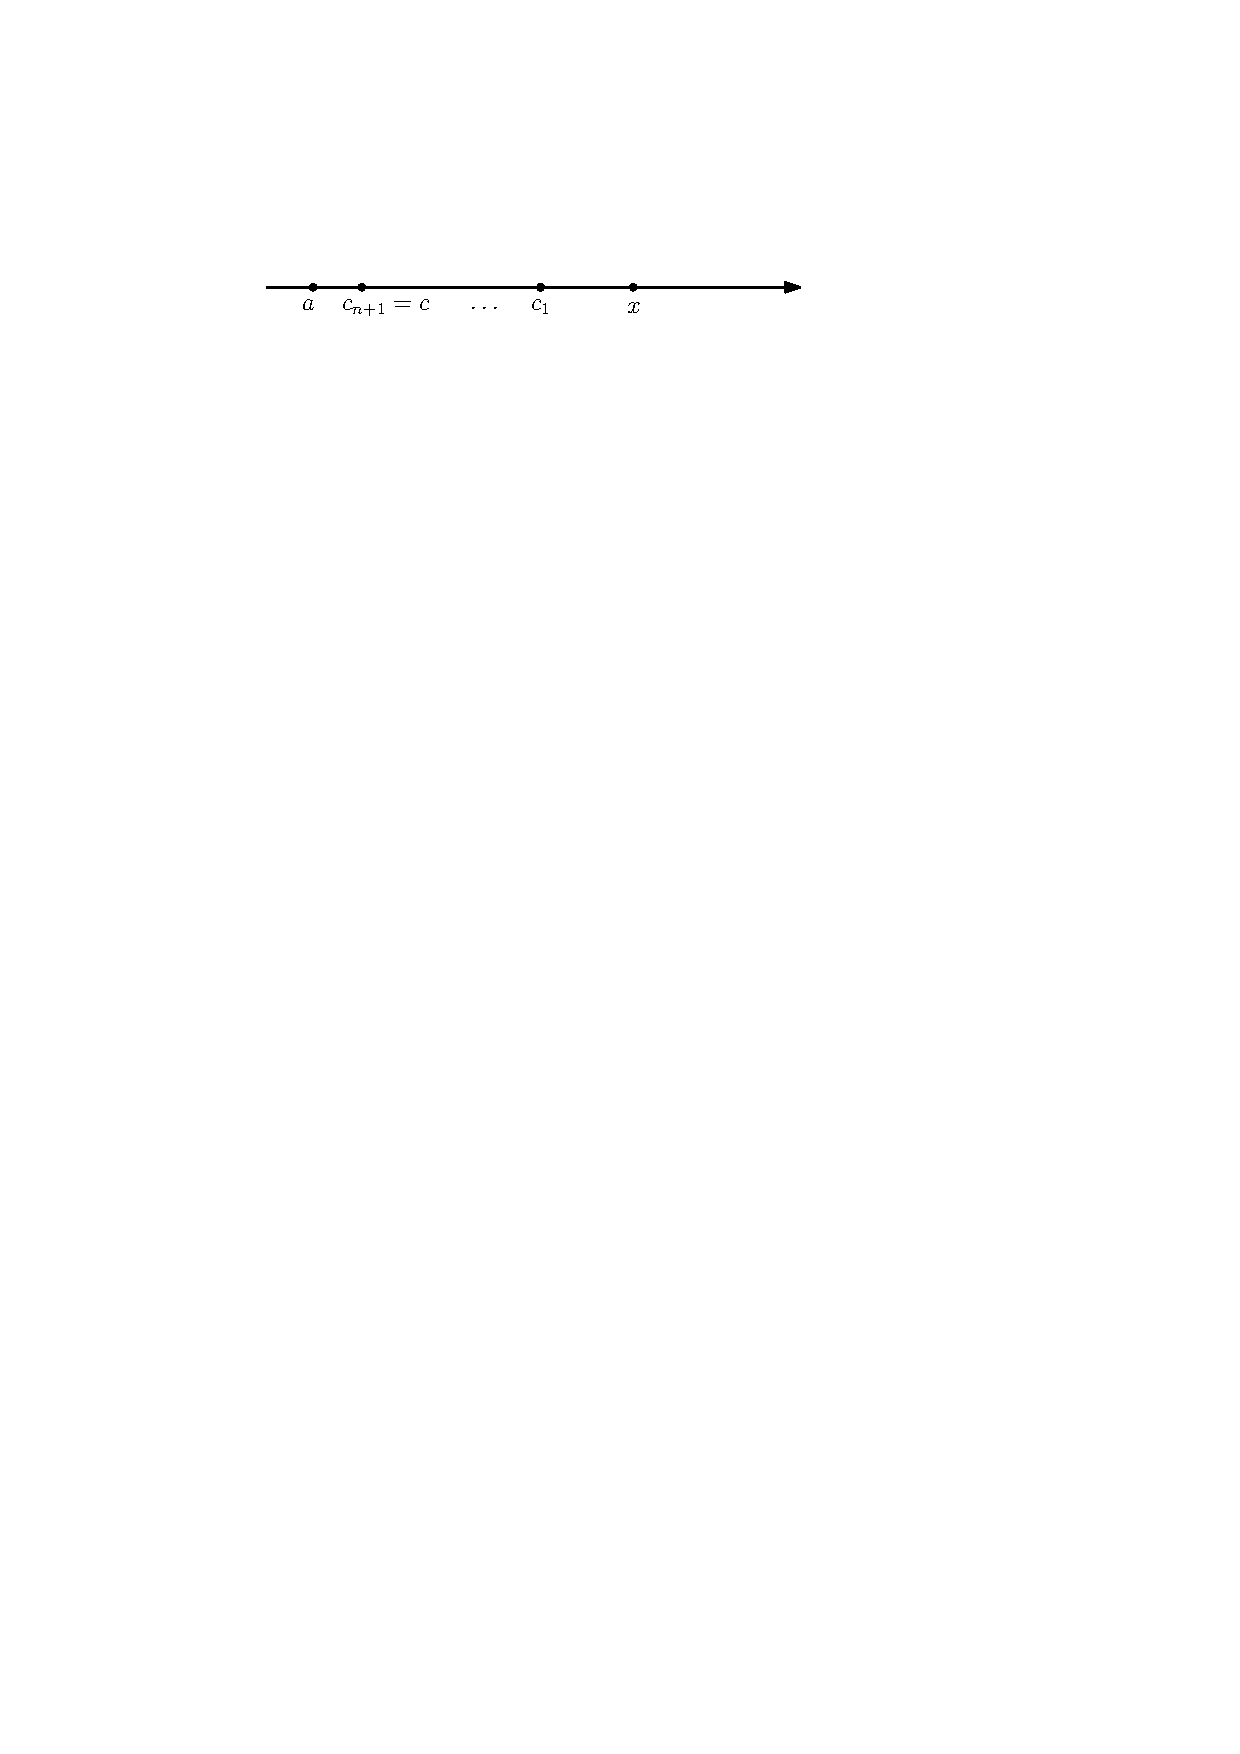
\includegraphics[width=0.5\linewidth]{taylor_lagrange}
  \item Выпуклость. 
    \resetall
    { \defn $X \subset \R^n$. X~--- выпуклое, если $\forall\,a,b\in X \; [a;b] \subset X $}
    { \lem Пусть $x,a,b \in \R^n$. Тогда $\forall\, x\in [a;b]\;\exists\, \theta \in [0;1] :
      x = a + \theta\,(b - a) $ }
    { \lem Пусть $x,a,b \in \R^n$. Тогда $\forall\, x\in [a;b]\;\exists\, \lambda_1,\lambda_2
      \in [0;1] : \lambda_1+\lambda_2 \land x = \lambda_1a + \lambda_2b $ }
    { \defn $f$ называется выпуклой (выпуклой вниз) на $I$, 
      если $ \{ (x;y) | x\in I, y\geq f(x) \}$"---~выпуклое множество.
      Почему-то почти не встречается обозначение $f \convex I$, 
      однако мне оно приглянулось $\smiley$}
    { \defn $f$ называется вогнутой (выпуклой вверх) на $I$, 
      если $ \{ (x;y) | x\in I, y\leq f(x) \}$"---~выпуклое множество.
      Аналогичные соображения про обозначение $f \concave I$ . } 
    
    \begin{thrm}[Условие выпуклости функции]
      Пусть $f : I \to \R$. Тогда  $f \convex I \Leftrightarrow \forall\,x_1,x_2\in I\;\\ 
      \forall\,\lambda_1,\lambda_2~\in~[0;1] : \lambda_1 + \lambda_2 = 1 \quad 
      f(\lambda_1x_1+\lambda_2x_2) \leq \lambda_1f(x_1) + \lambda_2f(x_2)$
    \end{thrm}

    \begin{lem}[О 3 хордах]
      Пусть $f : I \to \R,\; f \convex I,\; x_1, x,x_2\in I: x_1 < x < x_2$.
      Тогда и только тогда: 
      $$
        {f(x)-f(x_1)\over x-x_1} \leq {f(x_2)-f(x_1)\over x_2-x_1} \leq {f(x_2)-f(x)\over x_2-x} 
      $$
    \end{lem} Давайте объявим её очевидной из геометрии. 
    ( На самом деле она спокойно докажется из определения, но это длинно и не шибко интересно )
  \item Неравенство Енсена (Йенсена, Иенсена --- как только его не называют\dots)
    \resetall
    { \defn $x_1,\ldots,x_n\in I, \; \lambda_1,\ldots,\lambda_n\in[0;1],\;
      \sum\limits_{i=1}^n\lambda_i = 1$. \\
      Тогда $\displaystyle \sum_{i=1}^n\lambda_ix_i$~--- выпуклая комбинация.
    }
    { \rem $\sum\limits_{i=1}^n\lambda_ix_i \in I$ } 

    \begin{thrm}[Неравенство Енсена] \label{thrm:jensen}
      Пусть $f : I \to \R,\; f \convex I$. Тогда :
      \begin{align*}
        &\forall\,x_1,\ldots,x_n \in I,\; \forall\,\lambda_1,\dots,\lambda_n \in [0:1] 
                                          : \sum_{i=1}^n\lambda_i = 1 \quad
        f\left(\sum_{i=1}^n\lambda_ix_i\right) \leq \sum_{i=1}^n\lambda_if(x_i)
      \end{align*}
    \end{thrm} Индукцией побеждается
  \item Дифференциальные условия выпуклости.\\
    \resetall
    Поскольку теоремы кажутся очевидными, давайте их докажем.
    \begin{thrm} \label{thrm:derconvex} 
      Пусть $f \convex I=\langle a; b \rangle $. 
      Тогда: 
      \begin{enumerate}
        \item $x \in (a;b) \Rightarrow \exists f'(x-0), f'(x+0)$ и $f'(x-0) \leq f'(x+0)$.
        \item $x_1,x_2,x \in I,\;x_1<x_2 \Rightarrow f'(x_1+0) \leq f'(x_2-0)$
        \item $f\in C(a;b)$
      \end{enumerate}
    \end{thrm}
    \begin{ittproof}
      \begin{enumerate}
        \item Пусть $\varphi(h) := {f(x+h) - f(x) \over h}, 0\not\in \mathscr{D}(\varphi)$ \\
          $ \sphericalangle\; h_1, h_2 \in (a;b): h_1 < h_2 $.
          Пусть $ h_1 > 0 $.
          Переобозначим: $ y_1 := x, y := x + h_1, y_2 := x + h_2 $.\\
          По лемме о 3 хордах:
          \[
            {f(y)-f(y_1) \over y-y_1} \leq {f(y_2)-f(y_1) \over y_2-y_1}\Leftrightarrow
            {f(x+h_1) - f(x) \over h_1} \leq {f(x+h_2)-f(x) \over h_2}\Leftrightarrow
            \varphi(h_1) \leq \varphi(h_2)
          \]
          Аналогичное верно и для $h_1 < 0 < h_2$ и $h_1 < h_2 < 0$, таким образом
          $\varphi$ монотонна в $\overset{\circ}{U}(0)$ и непрерывна в ней. Все разрывы
          монотонной функции --- скачки. Тогда каждая из половинок монотонна и ограничена.
          А значит $\exists\, \varphi(+0), \varphi(-0)$ и равны $f'(x+0), f'(x-0)$ соответственно.
          При этом никто не гарантирует, что $\exists\, f'(x) = f'(x-0) = f'(x+0)$.
        \item По лемме о 3 хордах 
          \begin{align*}
            {f(x) - f(x_1) \over x - x_1} &\leq {f(x) - f(x_2)\over x - x_2} \\
            \scalebox{0.8}{($x\to x_1+0$)}\downarrow\quad &
            \qquad\downarrow \scalebox{0.8}{($x\to x_2-0$)} \\
            f'(x_1+0)                      &\leq f'(x_2-0)
          \end{align*}
        \item Так как существуют конечные $f'(x-0)$ и $f'(x+0)$, то $f(x-0)=f(x+0)=0$.
          То есть $f\in C(x)$. Однако нам ничего не известно про границы $I$. Заметим также,
          что число точек <<перелома>> не более чем счётно. Как было доказано ранее, в 
          точках, где не существует производная $f(x_0-0) < f(x_0+0)$. По теореме о полноте
          $\Q$ между ними есть $r\in \Q$. Также отметим, что $r_1 < f(x_1+0) < f(x_2-0) < r_2
          \Rightarrow r_1 < r_2$. Мы построили сюръекцию из $\Q$ в множество разрывов --- победа. 
      \end{enumerate}
    \end{ittproof}
    \begin{thrm} 
      Пусть $f : I\to \R,\; f\in C^1(I)$. Тогда $f \convex I \Leftrightarrow f' \uparrow I$.
    \end{thrm}
    \begin{ittproof}
      \begin{itemize}
        \item[\fbox{$\Rightarrow$}] следует из теоремы~\ref{thrm:derconvex}
        \item[\fbox{$\Leftarrow$}] Пусть $x_1 < x < x_2 \in I$. Из теоремы Лагранжа
        \begin{align*}
          \exists\, c_1\in (x_1,x), c_2 \in (x;x_2) : f'(c_1) = {f(x)-f(x_1)\over x-x_1},\;
          f'(c_2) = {f(x_2)-f(x)\over x_2-x} \Rightarrow \\ 
          {f(x)-f(x_1)\over x-x_1} \leq {f(x_2)-f(x)\over x_2-x}
        \end{align*} и по утверждению обратному к лемме о 3 хордах $f \convex I$ 
      \end{itemize}
    \end{ittproof}
    { \thrm Пусть $ f\in C^2(I)$. Тогда $f \convex I \Leftrightarrow f'' \geq 0 \text{ на } I$ }
  \item Неравенство Гёльдера
    \resetall
    \begin{thrm}
      $\forall\, a_1,\dots,a_n; b_1,\dots,b_n > 0 ,\; \forall\, p,q > 1: {1\over p}+{1\over q}=1$
      \[
        \sum_{i=1}^n a_ib_i \leq 
        \left( \sum_{i=1}^n a_i^p \right)^{1/p} \left( \sum_{i=1}^n b_i^q \right)^{1/q} 
      \]
    \end{thrm}
    Докажется через неравенство Енсена (при $p > 1$ $x^p \convex \R_+ $) не без помощи магии.
\end{enumerate}

\section*{Интегралы}

\begin{enumerate}
\setcounter{enumi}{50}
  \itemrange{1}  Первообразная и неопределённый интеграл.
    \resetall
    { \defn Пусть $f,F : I\to \R$. Тогда $F' = f \Leftrightarrow F$~--- первообразная для $f$.}
    { \thrm $f \in C(I) \Rightarrow \exists\, F : F' = f$ }
    { \thrm $F,G,f:I\to\R : F'=G'=f$. Тогда $F - G \equiv c (c\in\R)$.}
    { \defn Неопределённый интеграл $\int f(x)\,{\rm d}x := \{F(x) + c|c\in\R\, 
      F\text{ --- первообразная }f\} $ }
    
    Свойства первообразной:
    \begin{enumerate}
      \resetall
      \item $\displaystyle {\rm d} \int f(x)\,{\rm d} x = f(x)\,{\rm d}x$
      \item $\displaystyle \int {\rm d} F(x) = F(x)+c, c\in\R$
      \item $\displaystyle \int \alpha f(x) + \beta g(x)\,{\rm d}x = 
        \alpha\,\int f(x)\,{\rm d}x + \beta\,\int g(x)\,{\rm d}x$
      \item Формула интегрирования по частям.\\
        $\displaystyle u,v \in C^1(I) \Rightarrow \int u\,{\rm d}v = uv - \int v\,{\rm d}u$
      \item Замена переменной в неопределённом интеграле.\\
      Пусть $\varphi:I_t\to I,\; \varphi\in C^1(I_t),\; x=\varphi(t)$. Тогда 
      $\displaystyle \int f(x)\,{\rm d}x = \int (f \circ \varphi)(t)\,\varphi'(t){\rm d}t$
    \end{enumerate}
  \item Алгоритмические вопросы интегрирования
    \begin{thrm} \label{thrm:int_ratio}
      $\int R(x){\rm d}\,x$, где $R(x)\in\R(x)$~--- выражается через элементарные функции. 
    \end{thrm}
    \begin{ittproof}
      Основные пункты доказательства:
      \renewcommand{\labelenumii}{\Roman{enumii}.}
      \begin{enumerate}
        \item Представимость в виде суммы многочлена и простейших дробей 
        \item Интегрируемость $\displaystyle{A\over x-a}$
        \item Интегрируемость $\displaystyle{A\over (x-a)^n}$
        \item Интегрируемость $\displaystyle{Ax + B\over x^2 + px + q}$ 
          \begin{enumerate}
            \item $\displaystyle{2x + p \over x^2 + px + q }$
            \item $\displaystyle{1      \over x^2 + px + q}$
          \end{enumerate}
        \item Интегрируемость ${Ax + B\over (x^2 + px + q)^n}$
          \begin{enumerate}
            \item $\displaystyle{2x + p\over (x^2 + px + q)^n}$ 
            \item $\displaystyle{1     \over (x^2 + px + q)^n}$
            \begin{itemize}
              \item $\displaystyle{1\over (u^2+1)^n}$~--- берётся по частям, 
                понижая на каждом шаге степень знаменателя.
            \end{itemize}
          \end{enumerate}
      \end{enumerate}\renewcommand{\labelenumii}{(\alph{enumii})}
    \end{ittproof}
    \begin{thrm} \label{thrm:int_ratio_sin}
      $\int R(\sin x,\cos x)\,{\rm d}x$, где $R(u,v)\in\R(u,v)$~--- 
      выражается через элементарные функции.
    \end{thrm}
    \begin{ittproof}
      $\sphericalangle\; t = \tg{x\over 2}$. Тогда 
      \[
        \sin x = {2t\over 1+t^2}, \;
        \cos x = {1-t^2\over 1+t^2}, \text{ а } {\rm d}x = {2\over 1+t^2}\,{\rm d}t
      \]. 
      Таким образом \[
      R\left({2t\over 1+t^2}, {1-t^2\over 1+t^2}\right) \to \tilde{R}(t) \in \R(t)\].
    \end{ittproof}
    \begin{thrm} \label{thrm:int_ratio_sqrt_quadr}
      $\int R(x, \sqrt{ax^2+bx+c})\,{\rm d}x$, где $R(u,v)\in\R(u,v)$~--- 
      выражается через элементарные функции. 
    \end{thrm}
    \begin{ittproof}
      $\sphericalangle\; t = \sqrt{ax^2 + bx + c} + \sqrt{a}\,x$(\emph{подстановка Эйлера}).
      Тогда \[ 
        x = {t^2 -c \over 2\sqrt{a}\,t + b}, \;
        \sqrt{ax^2 + bx + c} = {\sqrt{a}\,t^2 + bt + c\sqrt{a}\over 2\sqrt{a}\,t + b},\;
        {\rm d}x = 2{\sqrt{a}\,t^2 + bt + c\sqrt{a}\over (2\sqrt{a}\,t + b)^2}\,{\rm d}t
      \]. Рационализация достигнута. 
    \end{ittproof}

    \begin{thrm} \label{thrm:int_ratio_nrt}
      $\int R(x, \root n \of{ax+b\over cx+d})\,
      {\rm d}x$, где $R(u,v)\in\R(u,v)$~--- выражается через элементарные функции. 
    \end{thrm}
    \begin{ittproof}
      $\sphericalangle\; t^n = {ax + b\over cx + d}\,x$.
      Тогда \[ 
        x = {dt^n - b \over a -ct^n}, \;
        \root n \of{ax+b\over cx+d} = t, \;
        {\rm d}x = {(a\,d-b\,c) \,n\,t^{n-1}\over ( c\,t^n - a )^2}{\rm d}\,t
      \]. Рационализация достигнута. 
    \end{ittproof}
  \item Определённый интеграл
    \resetall
    { \defn Пусть $f: I\to \R,\; f\in C(I)\; a,b\in I$ и $F$~---первообразная. Тогда
    \[
      \int_a^bf \equiv \int_a^bf(x)\,{\rm d}x := F(b) - F(a) 
    \](\emph{формула Ньютона-Лейбница}) }
    \hphantom{0} \\ Интересные свойства:
    \begin{enumerate}
      \item Совсем простые (написаны просто чтобы не забыть)
        \begin{itemize}
          \item линейность
          \item $\displaystyle a<c<b\in I\; \int_a^bf = \int_a^cf+\int_c^bf$
          \item $\displaystyle \int_a^bf = -\int_b^af$
          \item $\displaystyle \forall a\in I \int_a^af=0$
          \item (Теорема Барроу) $\displaystyle f\in C(I),\; a,x\in I \Rightarrow 
            {{\rm d}\over{\rm d}x} \int_a^xf = f$
        \end{itemize}
      \item Чуть сложнее (нужна невероятная теорема про неравенства и производные)
        \begin{itemize}
          \item $\displaystyle f \geqq 0,\; a\leq b \Rightarrow \int_a^bf \geq 0$
            (такой значок: $\leqq$~--- будет использоваться для функций для красоты) 
          \item $\displaystyle f \geqq 0,\; a < b,\; \int_a^bf > 0 
            \Rightarrow \exists\, c : f(c) > 0$
          \item $\displaystyle f \leqq g,\; a < b \Rightarrow \int_a^bf \leq \int_a^bg$
            (интегрирование неравенств)
          \item $\displaystyle |f| \leqq g,\; a \leq b \Rightarrow \left|\int_a^bf\right|
            \leq \int_a^bg$
          \item $\displaystyle a \leq b \Rightarrow \left|\int_a^bf\right| \leq \int_a^b|f|$
          \item $\displaystyle f \leqq M,\; a \leq b \Rightarrow \left|\int_a^bf\right| 
            \leq M(b - a)$ (ограниченность)
        \end{itemize}
      \item Почти такие же, как у неопределённого интеграла
        \begin{itemize}
          \item $\displaystyle \int_a^bu\,{\rm d}v = uv\Bigr|_a^b - \int_a^bv\,{\rm d}u$ 
          \item Замена переменной
            \begin{align*}
            &f:I\to\R, f\in C(I),\;\varphi: J\to I, \varphi\in C^1(J), \;
            a, b\in I,\; \alpha,\beta\in J:\varphi(\alpha) = a\land\varphi(\beta) = b, \\
            &\int_\alpha^\beta (f\circ\varphi)(t)\varphi'(t)\,{\rm d}t 
            = \int_a^b f(x)\,{\rm d}x
          \end{align*}
        \end{itemize}
    \end{enumerate}
  \item Теорема о среднем
    \resetall
    \begin{thrm}\label{thrm:int_average}
    Пусть $f, g \in C([a;b]),\; g \geq 0,\; g \not\equiv 0$. Тогда
    \[
      \exists\, c\in (a;b) : f(c) = {\int_a^bfg \over \int_a^bg}
    \]
    \end{thrm}
    Доказывается через теоремы Вейерштрасса и Больцано-Коши о непрерывной функции.

    { \defn Пусть $f\in C([a;b]), \; a < b$. Тогда 
    \[
      \langle f \rangle \equiv f_\text{ср} :=  {1\over b-a} \int_a^b f
    \] }

    {\thrm Пусть $f \in C([a;b])$. Тогда $\exists\, c\in (a;b) : f(c) = \langle f \rangle$.}
    См. теорему~\ref{thrm:int_average}.
  \item Интеграл как предел Римановых сумм
    { \defn Пусть $f\in C([a;b])\,\; a < x_1 < \dots < x_{n-1} < x_n = b,\; 
    \xi_i\in[x_i;x_{i+1]}$. Тогда 
    \begin{itemize}
      \item $\tau = \{x_1,\dots,x_{n-1}\}$~--- разбиение отрезка $[a;b]$
      \item $\xi = \{\xi_1,\dots,\xi_{n-1}\}$~--- оснащение разбиения $\tau$
      \item $\Delta x_i = x_{i+1}-x_i$~--- длина $i$-го отрезка
      \item $r=r(\tau) = \max\limits_i\{\Delta x_i\}$~--- ранг разбиения
      \item $\sigma = \sigma(\tau,\xi,f):= \sum\limits_{i=0}^{n-1}f(\xi_i)\cdot\Delta x_i$ ~---
        сумма Римана
    \end{itemize} }
    { \thrm Пусть $f:[a;b]\to\R,\; f\in C([a;b])$. 
      Тогда $\displaystyle\int_a^b f = \lim_{r(\tau)\to 0} \sigma(\tau,\xi,f)$ }
    Единственная теорема, для которой нужна равномерная непрерывность, так как $\delta$
    выбирается для всего разбиения сразу.
    Приближенные формулы:
    \begin{enumerate}
      \item Формула левых прямоугольников
        $x_i = a+i\,{b-a\over n},\; \Delta x_i = {b-a\over n} ,\; 
        \tau = \{x_i\}_{i=1}^{n-1},\; \xi_i=x_i$
        \[
          \int_a^bf \approx \sum_{i=0}^{n-1}f\left(a+i\,{b-a\over n}\right)\cdot{b-a\over n}
        \]
      \item Формула правых прямоугольников
        $x_i = a+i\,{b-a\over n},\; \Delta x_i = {b-a\over n} ,\; 
        \tau = \{x_i\}_{i=1}^{n-1},\; \xi_i=x_{i+1}$
        \[
          \int_a^bf \approx \sum_{i=0}^{n-1}f\left(a+(i+1)\,{b-a\over n}\right)\cdot{b-a\over n}
        \]
      \item Формула трапеций
        $x_i = a+i\,{b-a\over n},\; \Delta x_i = {b-a\over n} ,\; 
        \tau = \{x_i\}_{i=1}^{n-1},\;$ \par
        $\displaystyle \xi_i=c\in [x_i;x_{i+1}]:f(c)~=~{f(x_i)+f(x_{i+1}) \over2}$
        \[
          \int_a^bf \approx \sum_{i=0}^{n-1}{f(x_i)+f(x_{i+1})\over 2}\cdot{b-a\over n}
        \]
      \item Формула Симпсона
        $x_i = a+i\,{b-a\over n},\;\Delta x_i = {b-a\over n},\;\tau=\{x_i\}_{i=1}^{n-1},\;$\par 
        $\displaystyle \xi_i=c\in [x_i;x_{i+1}] : 
        f(c) = {f(x_i) + 4f\left({x + x_{i+1}\over 2} \right) + f(x_{i+1}) \over 6}$
        \[
          \int_a^bf \approx \sum_{i=0}^{n-1}{f(x_i) + 4f(x_{i + {1\over2}})+ f(x_{i+1})\over 6}
          \cdot{b-a\over n}
        \]
    \end{enumerate}
  \item Интегральная форма остаточного члена формулы Тейлора  
    { \thrm Пусть $f : I\to\R,\; f\in C^{n+1}(I),\; a\in I$. 
      Тогда:
      \begin{align*}
        f(x) &= T_n(x) + R_n(x), \\
        &\text{ где } T_n(x) = \sum_{k=0}^n\,\alpha_k(x-a)^k,  \\ 
        &R_n(x) = {1\over n!}\int_a^x f^{(n+1)}(t)(x-t)^{n+1}\,{\rm d}x ,\\
        &\alpha_k = {f^{(k)}(a) \over k!} 
      \end{align*} 
    } Докажется индукцией по $n$ с интегрированием по частям на каждом шаге
  \end{enumerate}
  Ещё, конечно, есть примечания, но там вроде всё уже знакомое.
  \newpage\thispagestyle{empty}\mbox{}
  \newpage\thispagestyle{empty}\mbox{}
  \centering
  
\includegraphics[width=1\linewidth]{keep-calm-and-may-the-force-be-with-you-35}
\end{document}
